\documentclass[a4paper, twoside, openany, oldfontcommands]{memoir}

\settocdepth{subsection}
\setsecnumdepth{subsection}

\usepackage{pgf,tikz,pgfplots}
\pgfplotsset{compat=1.15}
\usepackage{mathrsfs}
\usetikzlibrary{arrows}
\newcommand{\degre}{\ensuremath{^\circ}}
\usepackage{xeCJK}
\usepackage{fontspec}
\usepackage{enumitem}
\usepackage[utf8]{inputenc}
\usepackage{amsmath}
\usepackage{amssymb}
\usepackage{amsthm}
\usepackage{extarrows}
\usepackage{blindtext}
\usepackage{fancyhdr}
\usepackage[many]{tcolorbox}
\usepackage{setspace}
\usepackage{upgreek}
\usepackage{longtable}
\usepackage{bm}
\usepackage{tabularx}
\usepackage{graphicx}
\usepackage{hyperref}
\usepackage[export]{adjustbox}
\usepackage{float}
\usepackage{titlesec}
\usepackage{titletoc}
\usepackage{xCJKnumb}
\usepackage{pgfplots}
\usepackage{indentfirst}
\usepackage{multirow}
\usepackage{pdfpages}
\usepackage{caption}
\usepackage{hyperref}
\usepackage{lscape}
\usepackage{ulem}


\hypersetup{
    colorlinks=true,
    linkcolor=black,
    urlcolor=blue,
    citecolor=black,
}


\usepackage[
  top=2cm,
  bottom=2cm,
  left=2cm,
  right=3cm,
  headheight=17pt, % as per the warning by fancyhdr
  includehead,includefoot,
  heightrounded, % to avoid spurious underfull messages
]{geometry} 

\pagestyle{fancy}
\fancyhf{}%clear all headers and footers
\fancyhead[LE]{\slshape \rightmark}
\fancyhead[RO]{\slshape \leftmark}
\fancyhead[LO,RE]{\thepage}

\setCJKmainfont{Noto Sans CJK TC Regular}
%\setCJKmainfont{思源宋體} 
\newCJKfontfamily\Kai{標楷體}
\newCJKfontfamily\Song{思源宋體}

\renewcommand{\contentsname}{目錄}
\definecolor{chapter}{HTML}{05668D}



\renewcommand{\listfigurename}{圖目錄}
\renewcommand{\listtablename}{表目錄}
\renewcommand{\figurename}{圖}
\renewcommand{\tablename}{表}

\renewcommand{\chaptermark}[1]{\markboth{#1}{}}
\let\cleardoublepage=\clearpage

\tabcolsep=12pt 
\renewcommand{\arraystretch}{1.2}

\theoremstyle{definition}
\newtheorem{definition}{Definition}[section]
\usepackage{xcolor}

\definecolor{section}{HTML}{028090}
\definecolor{subsection}{HTML}{00A896}
\definecolor{subsubsection}{HTML}{EA7317}

%\chapterfont{\color{chapter}}
%\sectionfont{\color{section}}
%\subsectionfont{\color{subsection}}
%\subsubsectionfont{\color{subsubsection}}




\makeatletter
\newcommand{\chapterauthor}[1]{%
  {\parindent0pt\vspace*{-25pt}%
  \linespread{1.1}\large\scshape#1%
  \par\nobreak\vspace*{35pt}}
  \@afterheading%
}
\makeatother

\setlength{\parindent}{2em}
\setlength{\parskip}{1em}
\renewcommand{\baselinestretch}{1.1}

\begin{document}

\tableofcontents
\setcounter{chapter}{-1}
\chapter{營隊介紹}
\chapterauthor{熊熊兔兔}

\section{營隊規定}


\subsection{要遵守的規定}
\begin{enumerate}[label=\arabic*)]
\item 營隊時間為8/13$\sim$8/15 08:00$\sim$16:00 8/16 08:00$\sim$\underline{\textbf{19:00}},時間內請遵守一切規定與指示。
\item 活動範圍皆在科教館內,除非在隊輔指示下,否則禁止出館。
\item 部分大型活動會在武陵大陸上舉行,但請勿進入教學區(就是有教室的地方)。
\item 身體若有任何不適,立即通知身旁的隊輔。
\item 隨時攜帶名牌,否則須做勞動服務協助本營。
\item 你們身旁的隊輔皆為科學班的電神,盡量問他們問題吧!
\item 認真上課,這是非常難得的機會,我們篩掉了很多人,請自重。
\end{enumerate}

\subsection{認真要遵守的規定}
\begin{enumerate}[label=\arabic*)]
\item 各位是從異世界被選中的學員,科學班遭遇了空前的危機,維持和平的條約消失了!(熊熊:喔不!!!!)
\item 在這幾天的營隊中,在課程或活動後會頒發部分線索,最後獲得最多線索點數的小隊將成為優勝。
\item 線索會與所有本部之人分享,希望諸位能幫助科學班解決危機。
\item 各個小活動與最終任務皆有獎項,爭取優勝小隊的同時別忘記認真參與各活動與課程。(需事先閱讀最終遊戲之規則。)(兔兔:在倒數第二章喔)
\end{enumerate}
\newpage
\subsection{活動範圍}
主要的活動範圍都在科教館,請注意,育菁樓附近正在興建新大樓,請勿從施工區穿越,請走育菁樓及崇德樓中間的走道抵達科教館。
\begin{center}
\begin{figure}[H]
\centering
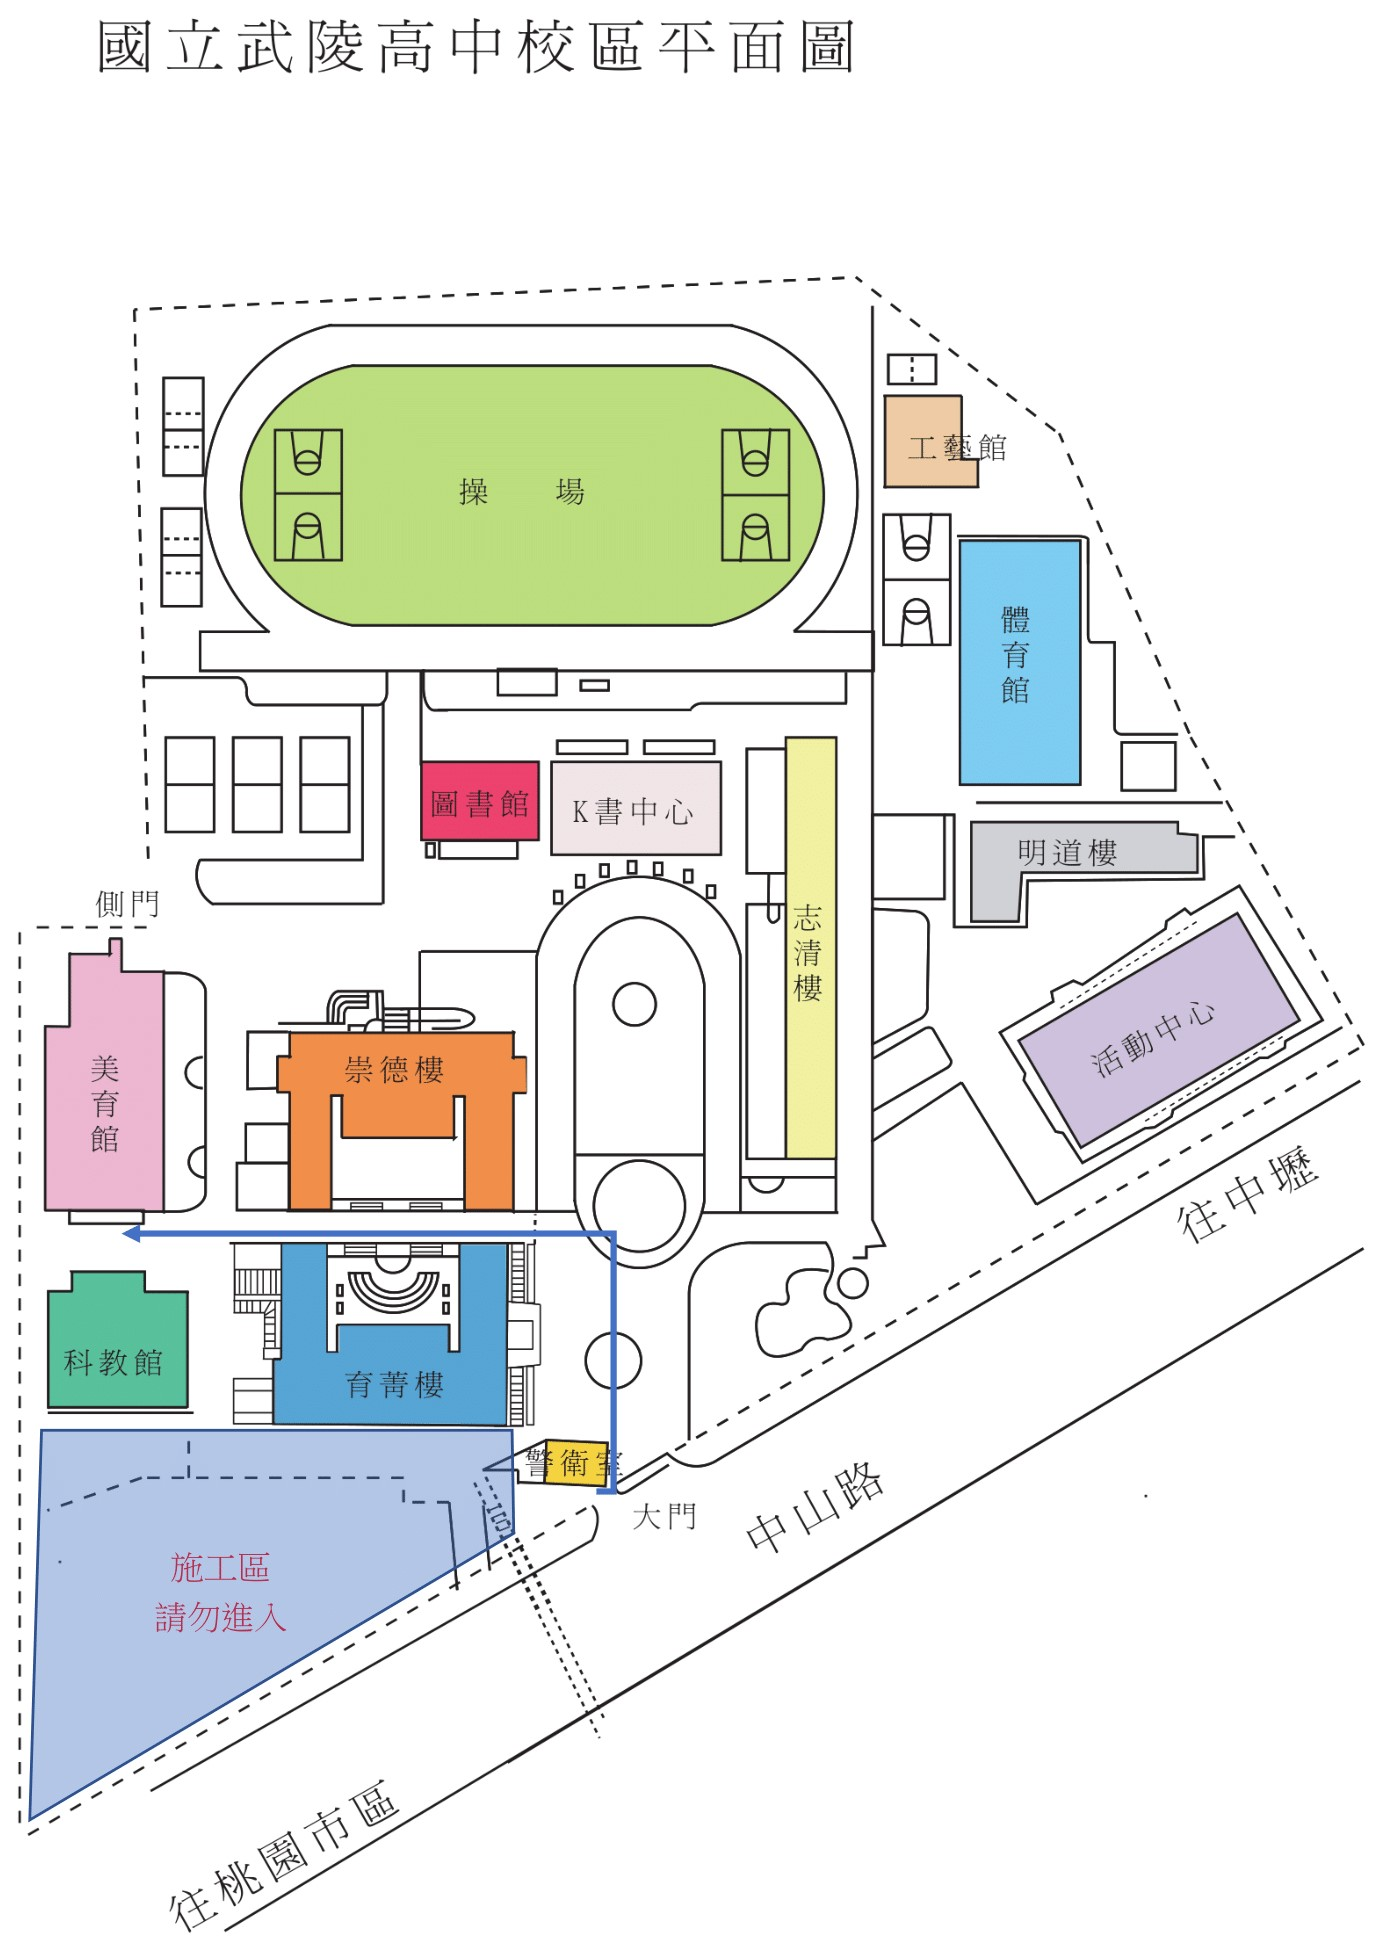
\includegraphics[width=15cm, center]{map.jpg}
\end{figure}
\end{center}
\section{日程}
\begin{table}[H]
\centering
\resizebox{10cm}{!}{%
\begin{tabular}{|c|c|c|}
\hline
\textbf{時間} & \multicolumn{2}{c|}{\textbf{8/13(二)}} \\ \hline
\textbf{8:00$\sim$8:50} & \multicolumn{2}{c|}{We Want You!} \\ \hline
\textbf{8:50$\sim$9:00} & \multicolumn{2}{c|}{Break} \\ \hline
\textbf{9:00$\sim$9:50} & \multicolumn{2}{c|}{武陵爭鬥的開端} \\ \hline
\textbf{9:50$\sim$10:00} & \multicolumn{2}{c|}{Break} \\ \hline
\multirow{4}{*}{\textbf{10:00$\sim$12:00}} & \multicolumn{2}{c|}{\multirow{4}{*}{真$\cdot$能力傳承}} \\
 & \multicolumn{2}{c|}{} \\
 & \multicolumn{2}{c|}{} \\
 & \multicolumn{2}{c|}{} \\ \hline
\textbf{12:00$\sim$12:30} & \multicolumn{2}{c|}{Lunch} \\ \hline
\textbf{12:30$\sim$12:55} & \multicolumn{2}{c|}{Nap} \\ \hline
\textbf{13:05$\sim$13:55} & \begin{tabular}[c]{@{}c@{}}我的改變\\ 你看的見\end{tabular} & 雪豹好可愛 \\ \hline
\textbf{13:55$\sim$14:05} & \multicolumn{2}{c|}{Break} \\ \hline
\textbf{14:05$\sim$14:55} & \multicolumn{2}{c|}{生輔} \\ \hline
\textbf{14:55$\sim$15:05} & \multicolumn{2}{c|}{Break} \\ \hline
\textbf{15:05$\sim$15:55} & 雪豹好可愛 & 所以…行! \\ \hline
\textbf{16:00$\sim$} & \multicolumn{2}{c|}{Home} \\ \hline
\end{tabular}%
}
\end{table}
% Please add the following required packages to your document preamble:
% \usepackage{multirow}
% \usepackage{graphicx}
\begin{table}[H]
\centering
\resizebox{\textwidth}{!}{%
\begin{tabular}{|c|c|c|c|c|c|c|}
\hline
\textbf{時間} & \multicolumn{2}{c|}{\textbf{8/14(三)}} & \multicolumn{2}{c|}{\textbf{8/15(四)}} & \multicolumn{2}{c|}{\textbf{8/16(五)}} \\ \hline
\textbf{08:00$\sim$08:15} & \multicolumn{6}{c|}{肌動蛋白的磷酸化與Z線的移動造成肝中丙酮酸再造} \\ \hline
\textbf{08:15$\sim$08:25} & \multicolumn{6}{c|}{Break} \\ \hline
\textbf{08:25$\sim$09:15} & \multicolumn{2}{c|}{\multirow{3}{*}{溶解度與克氏循環}} & 急急護法現身 & 幾何幾何? & 所以…行! & 焓是長來幹嘛的? \\ \cline{1-1} \cline{4-7} 
\textbf{09:15$\sim$09:25} & \multicolumn{2}{c|}{} & \multicolumn{4}{c|}{Break} \\ \cline{1-1} \cline{4-7} 
\textbf{09:25$\sim$10:15} & \multicolumn{2}{c|}{} & \multicolumn{2}{c|}{1A2B} & \multicolumn{2}{c|}{你該知道的事} \\ \hline
\textbf{10:15$\sim$10:20} & \multicolumn{6}{c|}{Break} \\ \hline
\textbf{10:20$\sim$11:10} & 霧裏看物理 & 急急護法現身 & \multicolumn{2}{c|}{\multirow{2}{*}{分身!!!!!}} & \multicolumn{2}{c|}{\multirow{2}{*}{波濤洶湧}} \\ \cline{1-3}
\textbf{11:10$\sim$12:00} & 幾何幾何? & \begin{tabular}[c]{@{}c@{}}我的改變\\ 你看的見\end{tabular} & \multicolumn{2}{c|}{} & \multicolumn{2}{c|}{} \\ \hline
\textbf{12:00$\sim$12:30} & \multicolumn{6}{c|}{Lunch} \\ \hline
\textbf{12:30$\sim$12:55} & \multicolumn{6}{c|}{Nap} \\ \hline
\textbf{13:05$\sim$13:55} & 焓是長來幹嘛的? & 霧裏看物理 & \multicolumn{2}{c|}{\multirow{5}{*}{時空裂縫}} & \multicolumn{2}{c|}{\multirow{3}{*}{武陵大陸的終章}} \\ \cline{1-3}
\textbf{13:55$\sim$14:05} & \multicolumn{2}{c|}{Break} & \multicolumn{2}{c|}{} & \multicolumn{2}{c|}{} \\ \cline{1-3}
\textbf{14:05$\sim$14:55} & \multicolumn{2}{c|}{\multirow{3}{*}{胖子與NaOH}} & \multicolumn{2}{c|}{} & \multicolumn{2}{c|}{} \\ \cline{1-1} \cline{6-7} 
\textbf{14:55$\sim$15:05} & \multicolumn{2}{c|}{} & \multicolumn{2}{c|}{} & \multicolumn{2}{c|}{Break} \\ \cline{1-1} \cline{6-7} 
\textbf{15:05$\sim$15:55} & \multicolumn{2}{c|}{} & \multicolumn{2}{c|}{} & \multicolumn{2}{c|}{The end?} \\ \hline
\textbf{16:00$\sim$} & \multicolumn{2}{c|}{Home} & \multicolumn{2}{c|}{Home} & \multicolumn{2}{c|}{\begin{tabular}[c]{@{}c@{}}16:00$\sim$19:00 \\ Final\end{tabular}} \\ \hline
\end{tabular}%
}
\end{table}
\section{小隊員\&隊輔}
% Please add the following required packages to your document preamble:
% \usepackage{graphicx}
\begin{table}[H]
\centering
\resizebox{\textwidth}{!}{%
\begin{tabular}{|c|c|c|c|c|c|c|c|c|}
\hline
\textbf{小隊} & \multicolumn{6}{c|}{\textbf{隊員}} & \multicolumn{2}{c|}{\textbf{隊輔}} \\ \hline
1 & 葉書佑 & 李澤暘 & 楊芷菱 & 游聿堂 & 童靖幃 & 蔡品昱 & 黃芃嫣 & 黃智笙 \\ \hline
2 & 羅大剛 & 許珍瑋 & 黎廷緯 & 陳思妤 & 林詩耕 & 許育晟 & 邱柏偉 & 葉欲禾 \\ \hline
3 & 周宇凡 & 林哲安 & 江伯翊 & 黃昱昇 & 黃柏瑜 & 楊瑄芸 & 鄧駿樺 & 柳凱馨 \\ \hline
4 & 林奕杉 & 陸柏蓉 & 林立恩 & 祁幃凱 & 林沅龍 & 李家勝 & 張智閎 & 蘇郁棻 \\ \hline
5 & 黃子倫 & 林佑瑋 & 呂紹頡 & 洪鈺翔 & 呂丞凱 & 吳奕萱 & 戴佑丞 & 鄧朝語 \\ \hline
6 & 李瑞恩 & 車亮萱 & 楊心澄 & 謝廷承 & 陳威廷 & 吳宇凡 & 林陽 & 胡睿喆 \\ \hline
7 & 徐震閎 & 林澄 & 柯儀寀 & 吳宇平 & 汪煒翔 & 吳孟學 & 蔡博恩 & 賴城諭 \\ \hline
\end{tabular}%
}
\end{table}
\section{積分表與積分表}
\begin{table}[H]
\begin{minipage}{0.5\linewidth}
\centering
\begin{tabular}{|c|c|c|}
\hline
時間點 & 獲得物 & 積分 \\ \hline
各課程優勝 & 小線索 & 15 \\ \hline
科教館裡藏的 & 線索碎片 & 5 \\ \hline
\multirow{2}{*}{1A2B 優勝} & 小線索 & 15 \\ \cline{2-3} 
 & 中線索 & 25 \\ \hline
\multirow{2}{*}{時空裂縫中} & 中線索 & 25 \\ \cline{2-3} 
 & 大線索 & 40 \\ \hline
\multirow{2}{*}{你該知道的事} & 小線索 & 15 \\ \cline{2-3} 
 & 中線索 & 25 \\ \hline
End Game & \multicolumn{2}{c|}{獨立計算} \\ \hline
\end{tabular}
\captionof{table}{積分表}
\end{minipage} \hfill
\begin{minipage}{0.45\linewidth}
\centering
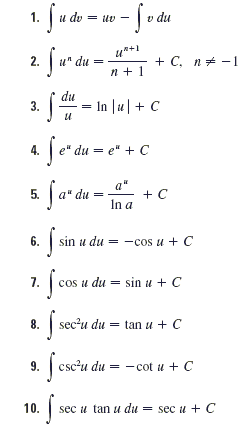
\includegraphics[width=\linewidth]{integral.png}
\captionof{figure}{積分表}
\label{fig:integral}
\end{minipage}
\end{table}


\let\cleardoublepage\clearpage
\part{物理}
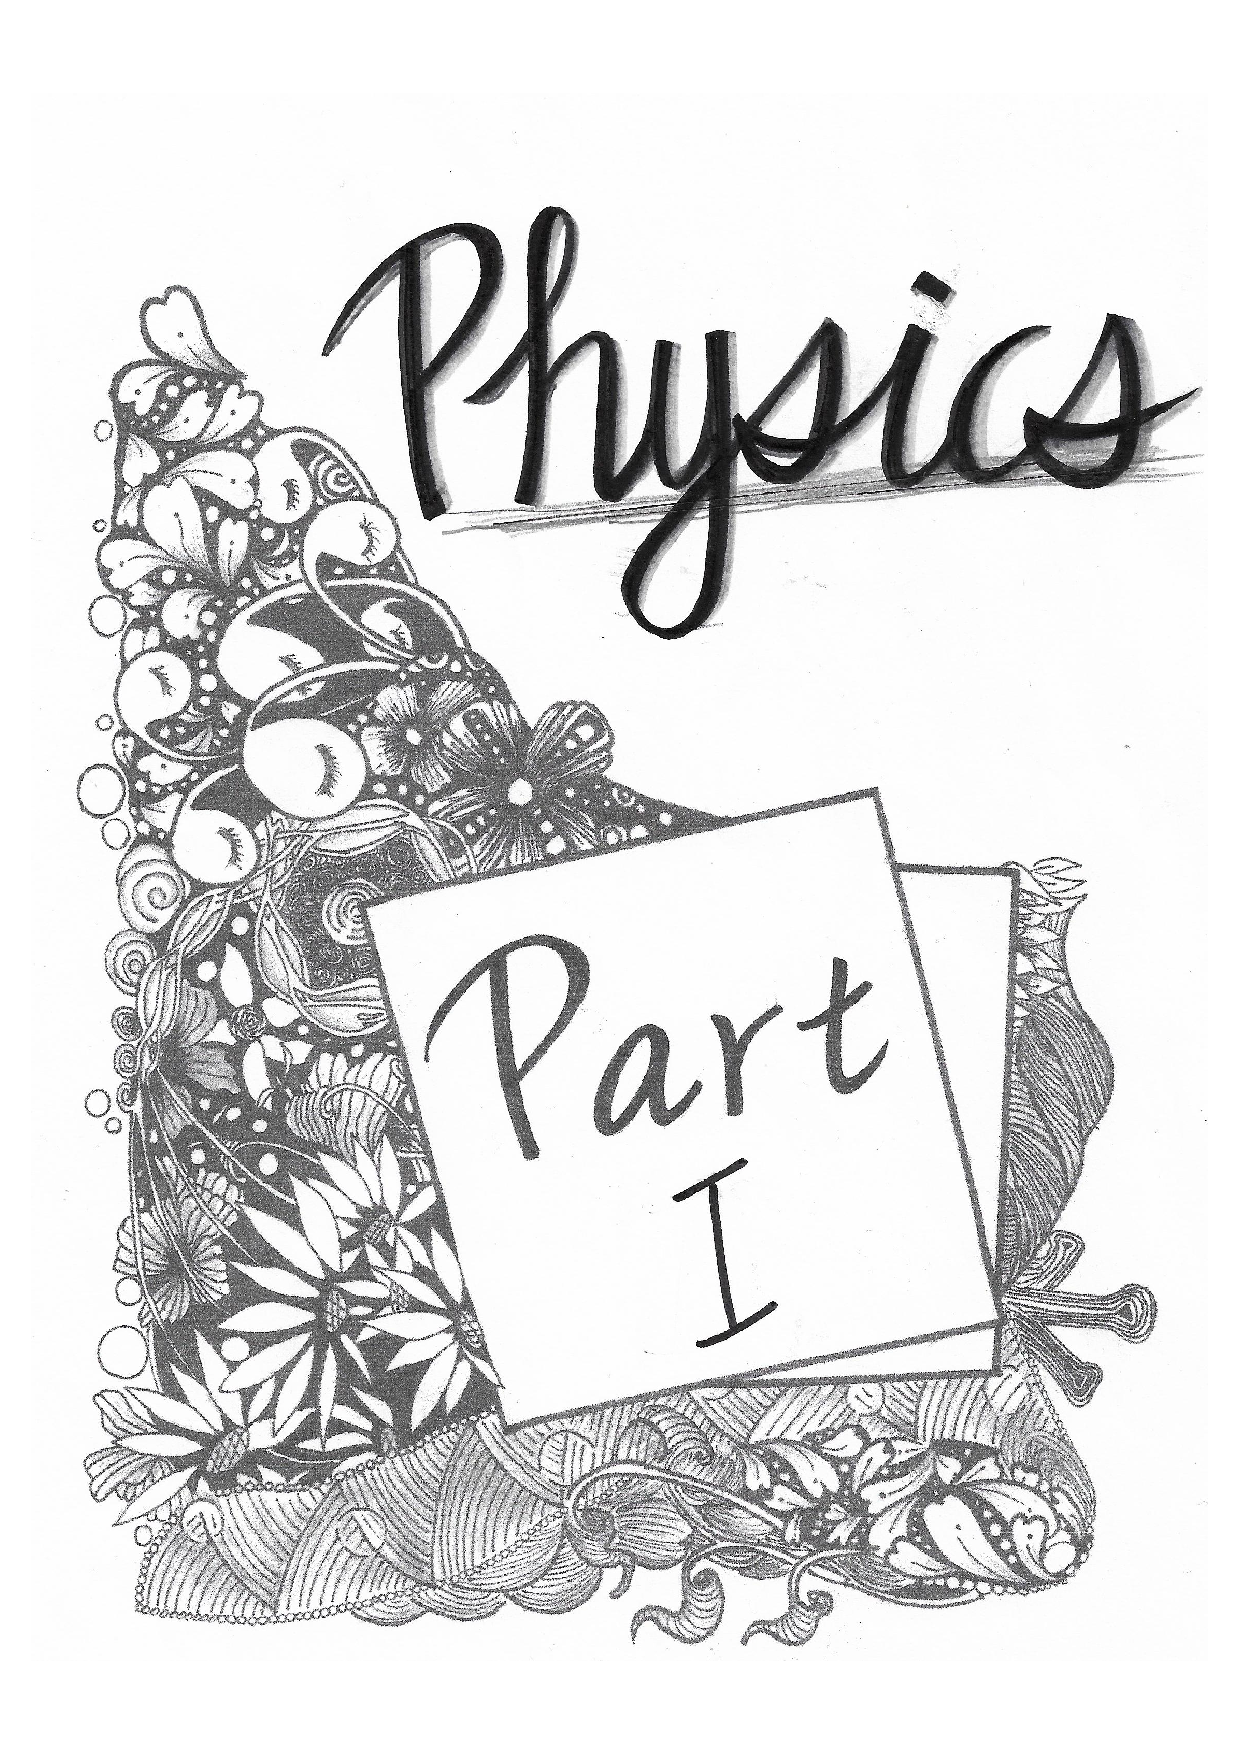
\includepdf[scale=0.9]{partImage/part1.pdf}
\chapter{霧裡看物理—擺}
\chapterauthor{張智閎}

\setcounter{section}{-1}
\section{前言}
Hi各位,我是熊熊,因為兔兔很懶不想打講義,所以叫編這本講義的熊熊隨便打一打,每個主題幫他留一頁空白就好,然後還給熊熊這些不合理的要求。
\begin{figure}[H]
\centering
\graphicspath{{physics/}}
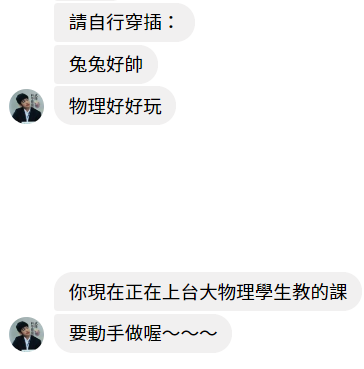
\includegraphics[width=7.5cm, center]{request.png}
\caption{不合理的要求} \vskip 10 pt
\label{fig:request}
\end{figure}
\newpage

\section{什麼是物理}
\newpage
\section{你該知道的事}
\newpage
\section{場?}
\newpage
\section{擺-1}
\newpage
\section{擺-2}
\newpage
\section{擺-3}
\newpage
\section{然後呢?}
\newpage

\newpage
\section{講師介紹}
\begin{itemize}
\item 姓名:張智閎
\item 性別:男
\item 特色:全班公認最電,高一去參加物奧選訓即獲得前半,保送台大物理(編按:本人表示自己不會念物理系)、偏矮,且從國小就如此、擔任圖資時,從不做事、幾乎所有自然科都免修,然後用免修的時間準備英文辯論或外交小尖兵,可謂不務正業的代表(編按:柏丞曰:「智閎感覺下學期不太認真耶」)、曾在緬甸與志工團隊同房睡時,講了整晚夢話,其中包括「草莓給我拿來」(編按:對講師大喊「草莓給我拿來」有機率獲得額外加成)。
\item 名言:我要看一下這題((寫,喔解出來、熊熊$\sim\sim\sim\sim$、熊熊你在幹嘛、草莓給我拿來。
\end{itemize}
\chapter{從波動認識物理}
\chapterauthor{丁安磊}

\section{一進一出:函數專論}

\subsection{為什麼?}

數學家發明了函數,為了討論兩種\textbf{變數}之間的\textbf{關係},而在物理的研究過程中,也常需要討論各個\textbf{物理量}之間的\textbf{關係}(物理量是變數的一種),函數是兩種變數之間的對應關係,大致概念如下圖所示。

\begin{figure}[H]
\centering
\graphicspath{{physics/}}
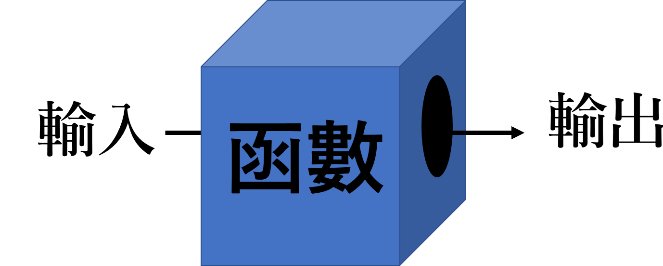
\includegraphics[width=5cm, center]{blackox.png}
\caption{把函數比喻成箱子,會將輸入的變數轉化為輸出的變數。} \vskip 10 pt
\label{fig:blackbox}
\end{figure}
\subsection{函數的呈現}

我們可以有許多方法呈現這這個箱子到底做了甚麼,以下列舉幾種。

\begin{enumerate}
	\item \textbf{文字:}
	\begin{enumerate}
		\item 圓面積與半徑的平方成正比
		\item 密度與質量成正比、與體積成反比
		\item 當體積固定密度與質量成正比
	\end{enumerate}
	\item \textbf{函數圖表:} \\
		例如: \\
		\begin{table}[H]
		\centering
		\begin{tabular}{|c|c|}
		\hline
		\textbf{正多邊形}      & \textbf{內角角度}  	    \\ \hline
		正三角形      & $60^\circ$    \\ \hline
		正四邊形      & $90^\circ$    \\ \hline
		正五邊形      & $108^\circ$    \\ \hline
		正六邊形      & $120^\circ$    \\ \hline
         $\vdots $ &  $\vdots $     \\ \hline
		你爽的話可以繼續寫 & 可是我好懶 \\ \hline
	
		\end{tabular}
		\end{table}
	\item \textbf{函數圖形:}\\
當我們劃出圖形的表格,我們能夠把他標示在有由$x$軸和$y$軸形成的平面上。以$y=x^2$為例,一開始我們計算$x$和$y$的幾個對應關係,把它畫在平面上,接著越算越多,我們就能預測並畫出$y=x^2$的圖形。
\begin{figure}[H]
\centering
\graphicspath{{physics/}}
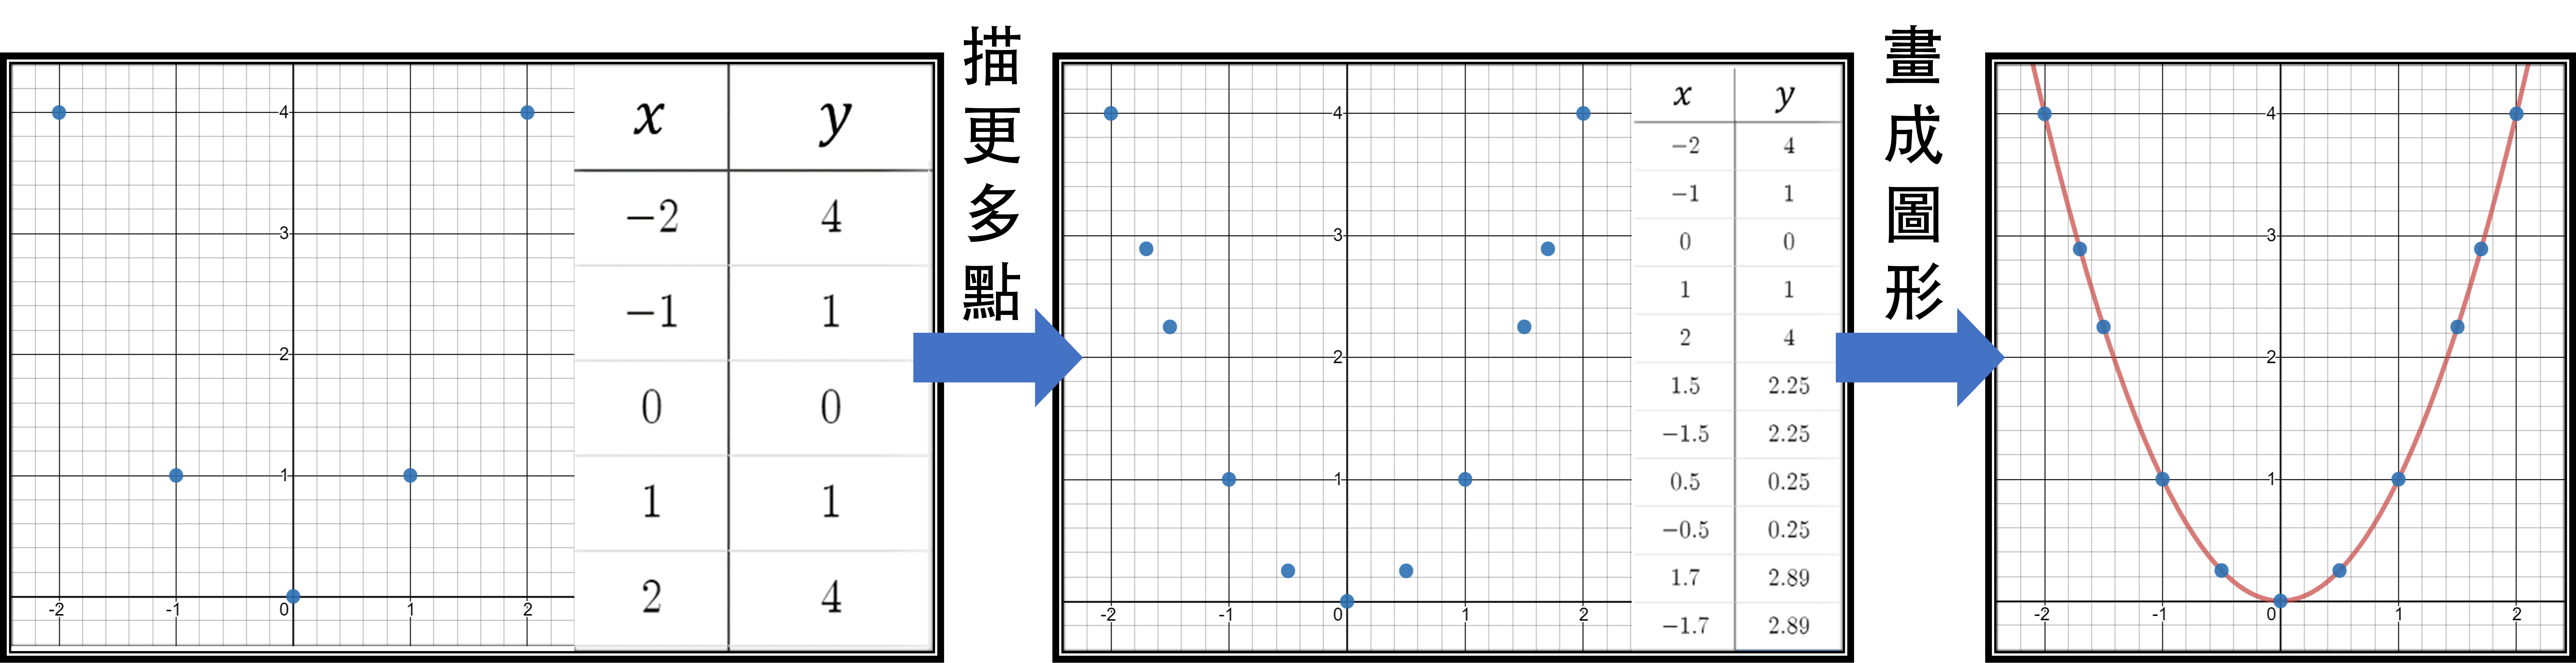
\includegraphics[width=\textwidth, center]{function_graph.png}
\label{fig:function1}
\end{figure}

	\item \textbf{數學式:} \\
這裡就舉幾個數學和物理常用到的公式來理解吧。
		\begin{figure}[H]
		\centering
		\graphicspath{{physics/}}
		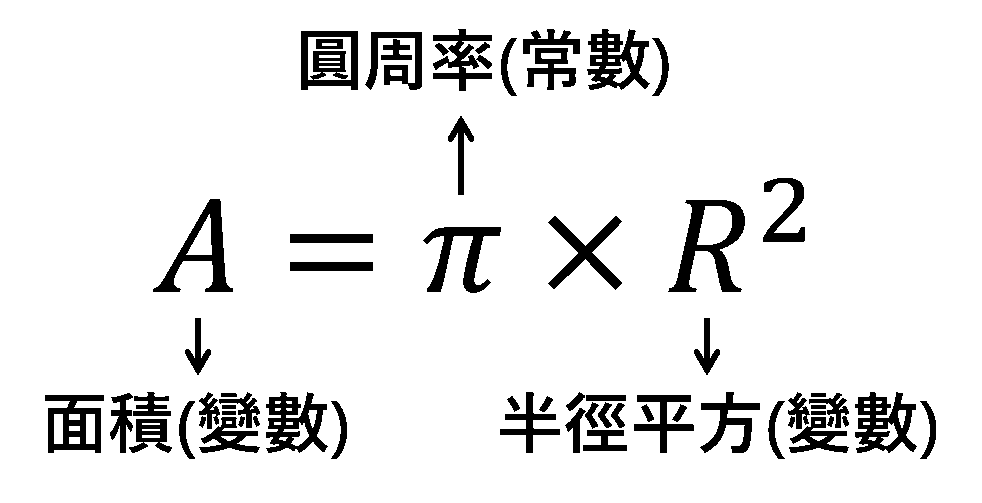
\includegraphics[width=5cm, center]{A.png}
		\caption{$A=f(R)$} \vskip 10 pt
		\label{fig:A}
		\end{figure}
				
		\begin{figure}[H]
		\centering
		\graphicspath{{physics/}}
		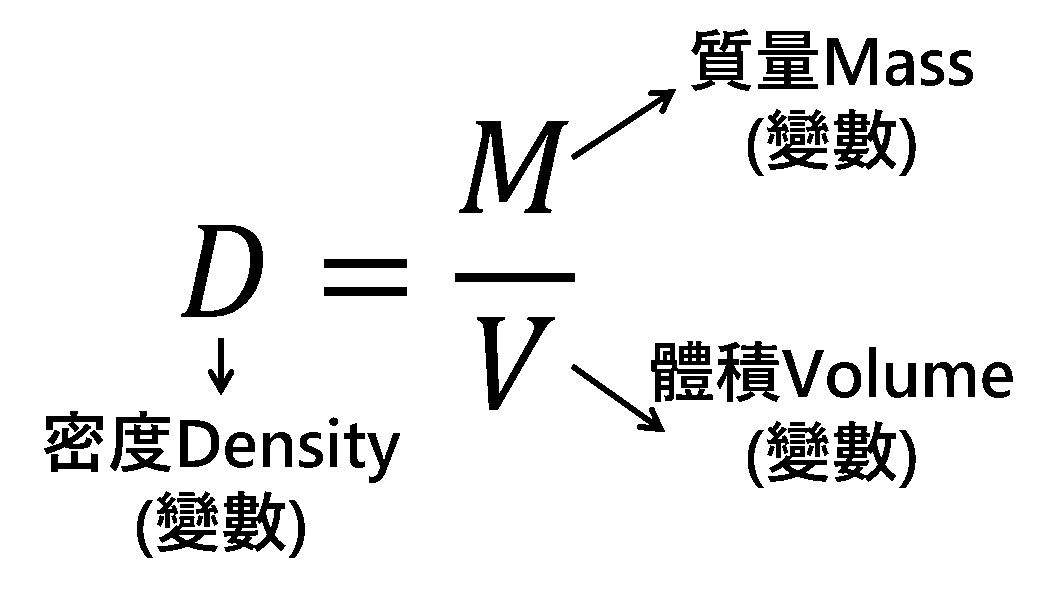
\includegraphics[width=5cm, center]{D1.png}
		\caption{$D=f(V,M)$} \vskip 10 pt
		\label{fig:D1}
		\end{figure}
		
		\begin{figure}[H]
		\centering
		\graphicspath{{physics/}}
		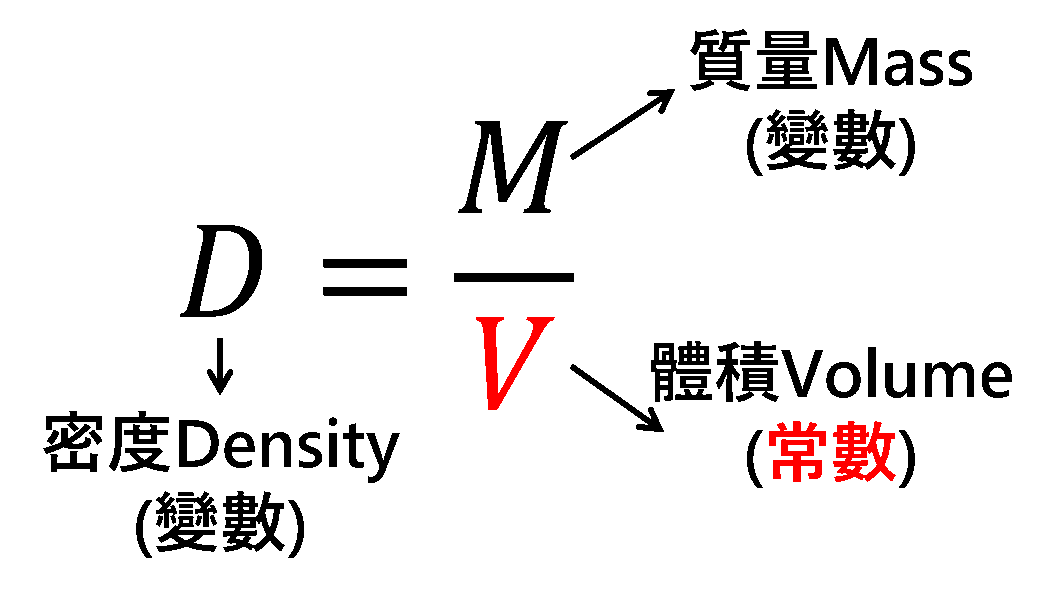
\includegraphics[width=5cm, center]{D2.png}
		\caption{$D=f(M)$} \vskip 10 pt
		\label{fig:D2}
		\end{figure}
\end{enumerate}

\section{聽起來很厲害:三角函數}
\subsection{複習:直角三角形的三角函數}
\begin{figure}[H]
\centering
\graphicspath{{physics/}}
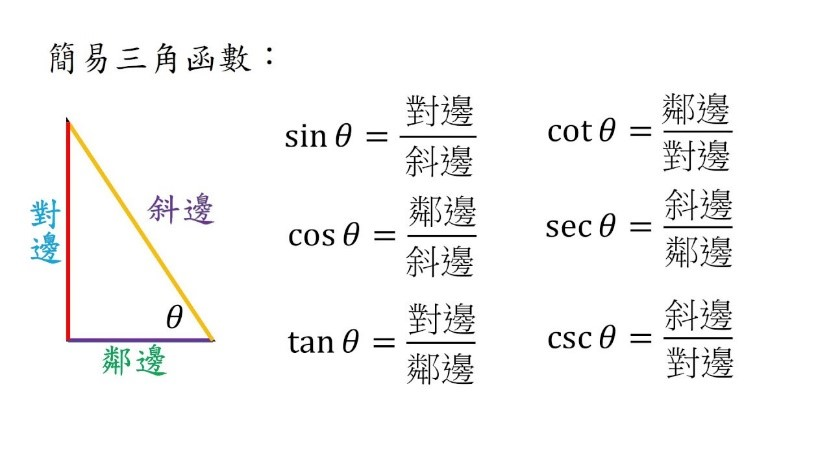
\includegraphics[width=7.5cm, center]{tri-function.jpg}
\caption{簡易三角函數} \vskip 10 pt
\label{fig:tri-function}
\end{figure}
\subsection{角的度量、換算與方向:}
\subsubsection{度($360^\circ$制)}
相信大家學過360°是什麼意思了,那為什麼要用360這個數字呢?因為古巴比倫人是用60進位,然後地球公轉差不多花360多天,這樣每天太陽差不多動一度,還有如果不是用360這種漂亮的數字的話,上面的正多邊形內角的表的數字就會很醜,我就不想打講義了。
\subsubsection{弧度(弳度制)}
在物理上,我們多使用弧度來度量角,弧度的定義如下:

\begin{center}
{\Kai 在圓周上,截取與半徑等長之弧,則此弧所對的圓心角稱為一弧度(或稱為一弳)} 
\end{center}

\noindent
因為科學家都很懶,以弧度為單位表示會省略單位。\\
所以我們看到角有度就是度,看到沒度就是弧度(?\\

\subsubsection{換算}
又因為單位圓的周長為$2\pi$,所以$360^\circ=2\pi$由此可得$1=(360^\circ )/2\pi \approx 57.29^\circ$,且$1^\circ=\frac{2\pi}{360^\circ}=0.0174533$。
\begin{figure}[H]
\centering
\graphicspath{{physics/}}
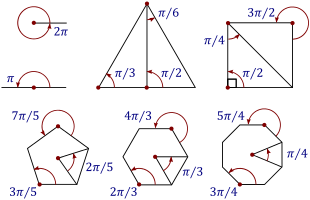
\includegraphics[width=7.5cm, center]{num-shape.png}
\caption{可以自己驗證看看} \vskip 10 pt
\label{fig:num-shape}
\end{figure}
\subsubsection{有向角}
以前我們學的角度不討論方向,但為了後面的廣義三角函數,我們定義角度的方向逆時針。
至於為什麼角度要這樣定義呢,等等就知道。 

所以一條線(始邊)繞著一個點旋轉後,變成另一條線(終邊),如果他逆時針轉,角度為正值,反之則為負值。

\begin{figure}[H]
\centering
\graphicspath{{physics/}}
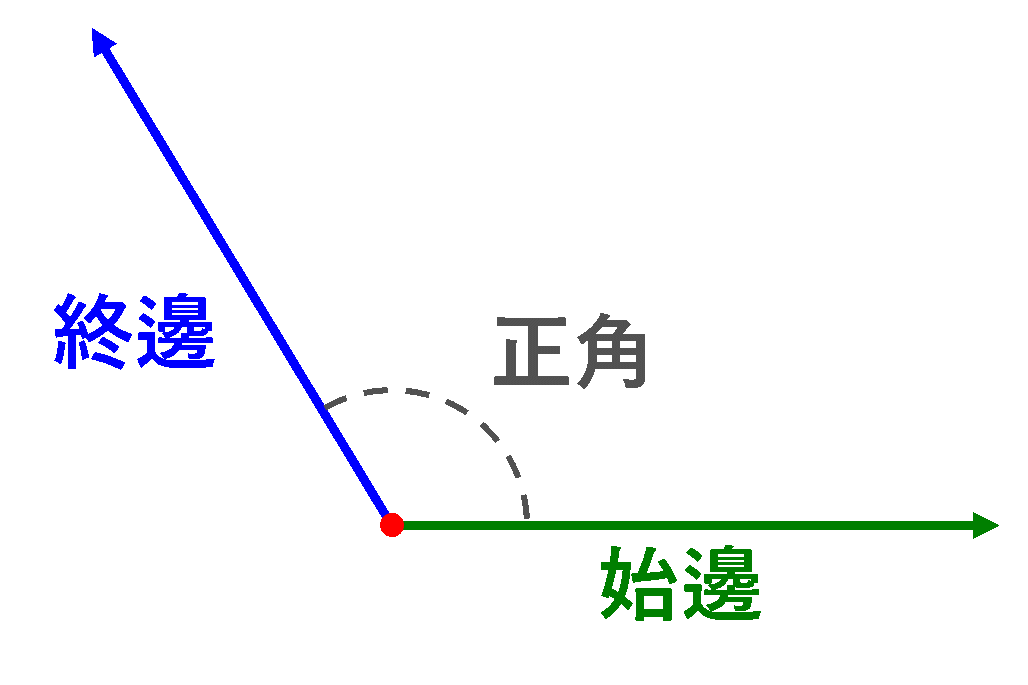
\includegraphics[width=7.5cm, center]{pos-angle.png}
\caption{正角} \vskip 10 pt
\label{fig:pos-angle}
\end{figure}

\begin{figure}[H]
\centering
\graphicspath{{physics/}}
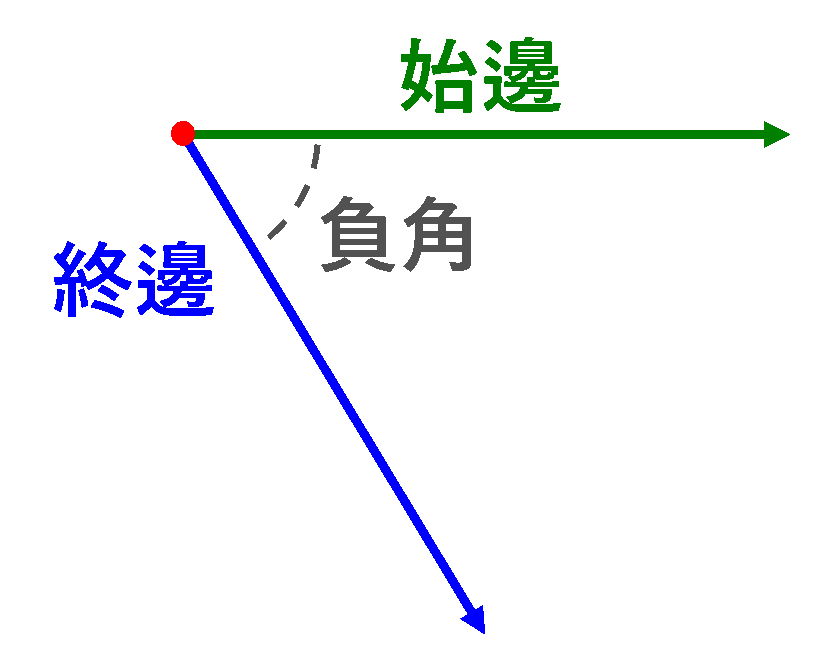
\includegraphics[width=7.5cm, center]{neg-angle.png}
\caption{負角} \vskip 10 pt
\label{fig:neg-angle}
\end{figure}

\noindent
\fbox{小測驗}
\begin{enumerate}
\item 這張圖中的廣義角是多少?
\begin{figure}[H]
\centering
\graphicspath{{physics/}}
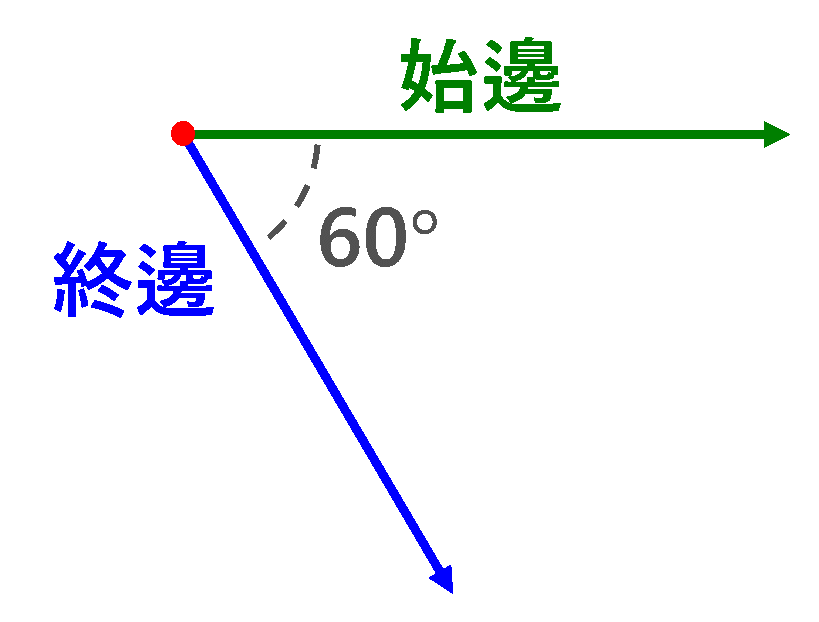
\includegraphics[width=7.5cm, center]{angle-test.png}
\label{fig:angle-test}
\end{figure}
\item 過了兩天,時鐘上的時針分針秒針轉了多少?
\end{enumerate}

\subsubsection{廣義三角函數}
在討論簡易三角函數的時候,我們無論如何都不能超過$90^\circ$
\begin{figure}[H]
\centering
\graphicspath{{physics/}}

\includegraphics[width=7.5cm, center]{over-90-tri.png}
\caption{怎麼壓都不會超過$90^\circ$} \vskip 10 pt
\label{fig:neg-angle}
\end{figure}

於是數學家為了推廣,使用單位圓定義三角函數
\begin{center}
\begin{equation*}
   \addtolength{\fboxsep}{5pt}
    \boxed{
    \begin{gathered}
   		\mbox{單位圓(半徑為1)上的一點,繞轉了}\theta \mbox{時,} \\
   		\mbox{使用此點的x,y座標定義三角函數:} \\
		x=\cos \theta \\
		y=\sin \theta 
    \end{gathered}
    }
\end{equation*}
\end{center}

這樣做的話,$\theta$在$0^\circ \sim 90^\circ$的範圍內,保持和簡易三角函數一樣,又能突破原本的限制。

\begin{figure}[H]
\centering
\graphicspath{{physics/}}
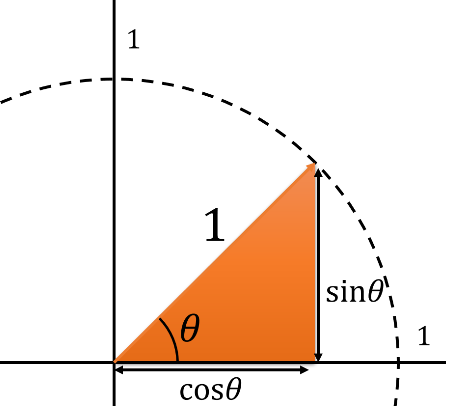
\includegraphics[width=7.5cm, center]{broad-tri-function.png}
\caption{廣義三角函數} \vskip 10 pt
\label{fig:broad-tri-function}
\end{figure}

\noindent
\fbox{小測驗}
\begin{enumerate}
\item $\sin (120^\circ)=$?,$\sin (\frac{2}{3} \pi)=$?
\item $\sin (\theta) = \frac{1}{2}$,$\theta =$?
\end{enumerate}

\subsection{三角函數的度量}
我們剛剛推廣了三角函數,本來我們的三角函數只能吃$0$到$\frac{\pi}{2}$之間的角度,但推廣之後任何數都可以是三角函數的輸入值,所以可以畫出函數的關係圖,六種三角函數都可以畫圖,不過我們先來關心最基本的:$\sin$函數圖(正弦函數圖)\\

要如何畫出$\sin$函數圖呢?課本裡通常使用無聊的描點法,不過這堂課已經夠無聊了,所以用投影的方法來想。

\begin{figure}[H]
\centering
\graphicspath{{physics/}}
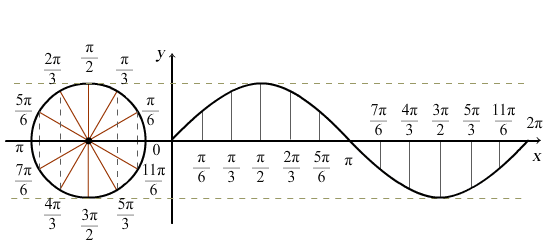
\includegraphics[width=\textwidth, center]{sin-wave.png}
\caption{$y=\sin (x)$} \vskip 10 pt
\label{fig:sin-wave}
\end{figure}

這是$y=\sin⁡ (x)$的圖畫出來的樣子,圖片是靜態的所以看起來很難,附錄裡有簡報檔案的網址可以慢慢看裡面的動畫。因為圓上的點繞了一圈會回到原點,所以後面的圖是無限重複的,我們稱$\sin$函數具有週期性,其週期為$2\pi$。

這個函數看起來很像波。事實上,在物理學,正弦波是最基本的一種波。

\section{波的計算方法}

\subsection{國中的波公式}
$$v=\frac{\lambda}{T}=\lambda f$$
\begin{center}
($v$;波速;$\lambda$:波長;$T$:週期;$f$:頻率)
\end{center}
\subsection{更BANG的波公式}
\subsubsection{簡介}
國中的波公式只能描述波速、波長、週期、頻率之間的關係,物理學家當然不會滿足,所以我們必須學習更高階的公式來描述波。

我們能夠最直接看到的就是波的偏移,以繩波為例,繩波是透過繩子作為介質傳遞的(廢話),如果我們在繩子上一點綁了一個紅色的結,如果繩子的波源例如拉繩子的手,只有上下移動,沒有左右移動,從旁邊看這個紅色的結只會上下移動,也就是說,只有波形會傳遞,介質只會上下震動並不會傳遞。

再舉一個例子聲波是空氣分子震動產生的,你可以想像敲鑼打鼓等等樂器的演奏,敲這些樂器你會讓他開始震動,於是他就會壓縮、然後放鬆(?)空氣分子,然後他的偏移(壓縮的幅度)如果越大則聲音傳到我們耳朵裡就會聽起來會越大聲

\subsubsection{與時間無關的偏移函數}
以下開始討論波的偏移與其他物理量的關係,一樣以最簡單的繩波為例,當波源製造出了正弦的繩波,按下時間暫停器,這個時候波的偏移和什麼物理量有關係?當然,是位置,不同位置的偏移量不同,所以我們可以把它們的函數這樣寫。

$$y=A \times \sin (x) \mbox{(振幅為A的正弦波)}$$
\begin{center}
($y$:偏移量;$x$:到波源的距離)
\end{center}


首先從$A$說起,在定義正弦函數的時候,我們是用單位圓,所以他會在1到-1之間震盪,但繩波的震幅不一定是1公尺,所以乘上一個$A$,稱為振幅,乘上$A$之後,繩波變成在$A\sim -A$之間震盪。


再來是$k$,同樣的,因為使用單位圓定義,所以正弦波的波長原本是$2\pi$,即一圈的角度,但繩波的波長不一定是$2\pi$公尺,所以我們要對正弦波進行拉伸,把他的波長伸長或縮短成$\lambda$。

那麼$k$要是多少才能有讓波長變成$\lambda$呢?也就是說$k$和$\lambda$的關係是什麼?

我們剛剛知道,$\sin$裡面包的是指一個角度,我們稱為\textbf{相角},所以對這個函數來說,$\sin$裡面包的是$kx$,我們把他當成單位圓上某點的的角度,當$x$逐漸增大,$kx$這個相角也開始改變,而且如果我們已知這個波的波長為$\lambda$,所以當$x$從0慢慢增加到$\lambda$的時候,$kx$也剛好走了一圈($2\pi$),所以會有

$$
k \times \lambda-k \times 0=2 \pi
$$

所以
$$ k = \frac{2\pi}{\lambda} $$

於是我們就推出來$k$與$\lambda$的關係,你可能會發現,我特別把$k\times0$這一項標出來,為什麼呢?因為你的起點可以任意決定。
比方說,對跟剛剛一樣的波做分析,其實我們也可以把$x$從$x_0$慢慢增加到$x_0+\lambda$時($x_0$代表隨便選的一個初始位置,我們喜歡用下標一個零代表初始,注意,$x$是變數,而$x_0$是常數),會有一樣的結果,因為$x_0$這一項會被消掉。
\begin{figure}[H]
\centering
\graphicspath{{physics/}}
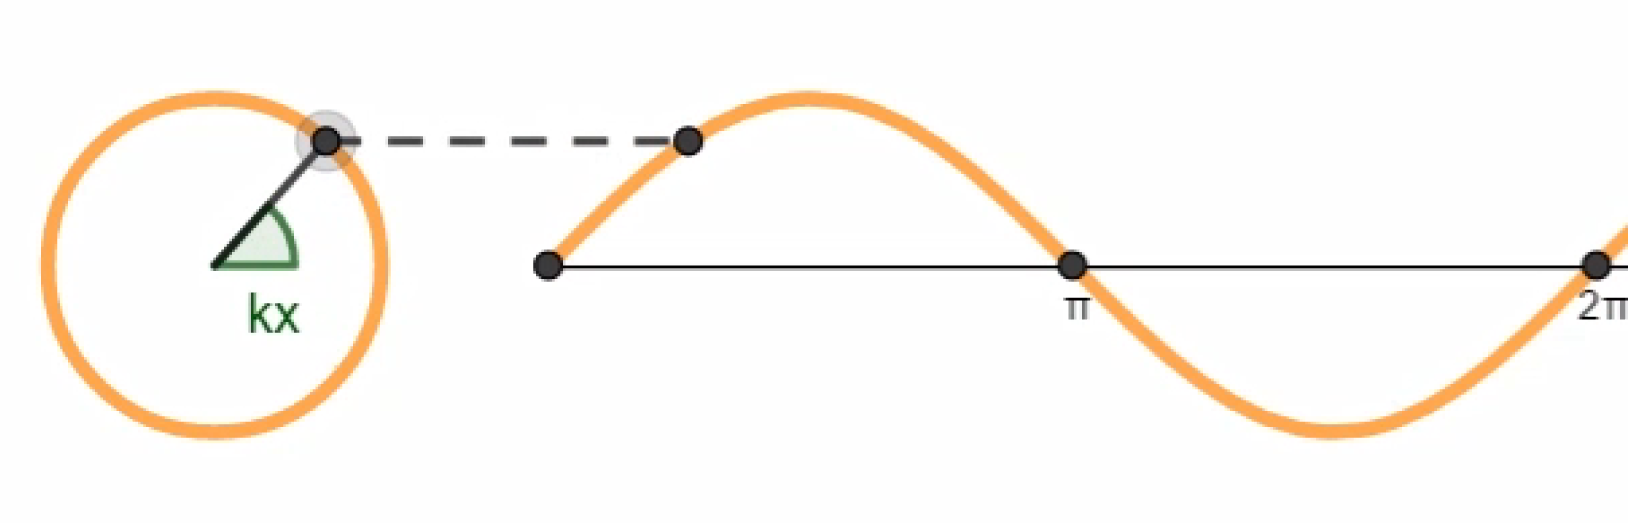
\includegraphics[width=\textwidth, center]{circle-wave.png}
\caption{示意圖,請注意右邊的座標軸是表示$kx$而不是$x$} \vskip 10 pt
\label{fig:circle-wave}
\end{figure}

\subsubsection{與時間有關的偏移函數}
物理學家很貪心,連時間也要討論,不過我們可以使用剛剛討論出的結果來分析與時間有關的偏移函數,我們知道,一段時間可以由無限多個的瞬間來組成,比喻成相片和影片的話大概就是這樣:

與前面類似,我們看只和時間有關的$\sin$函數。
$$ y = \sin (\omega t) $$

同樣,因為波的週期不是$2\pi$,所以要乘上一個數$\omega$,念作omega這裡所指的週期和上面有點不太一樣,上面的是指位置上的周期,而這裡是指時間上的週期,位置上的週期就是你\textbf{某一瞬間看到的(固定時間)}波形走多長會循環一次,而時間的週期就是指對於繩子上\textbf{某一點(固定位置)}時間過多久會回到原點(循環一次),以類似的方法尋找$ω$與$T$的關係。(注意這邊$t$代表時間,是變數;而$T$代表週期,是已經決定於波的常數)

所以對這個函數來說,$\sin$裡面包的是$\omega t$,我們把他當成單位圓上某點的的角度,當$t$逐漸增大,$\omega t$這個相角也開始改變,而且如果我們已知這個波的週期為$T$,所以當$t$從$t_0$慢慢增加到$t_0+T$的時候,$\omega t$也剛好走了一圈($2\pi$),所以會有
$$
\omega\left(t_{0}+T\right)-\omega\left(t_{0}\right)=2 \pi
$$

所以
$$
\omega=\frac{2 \pi}{T}
$$

{\Kai 【想想看,$x_0$,$t_0$的值有什麼意義?】}

\section{波的現象}
\begin{enumerate}
\item \textbf{波的疊加}:當兩個繩波相遇時,兩個波的偏移是可以疊加的,如果一個是高,一個是低,就像是兩側都有人在拉你一樣,會完全消除,如果兩個同為高,或同為低,疊在一起就會變得更高或更低。


\item \textbf{駐波}:如果繩子上有兩個反向但一樣的波,反向的通常是因為波的反射造成的,那麼他就會形成駐波,如下圖所示,任何你所看到的樂器幾乎都是基於駐波的原理。上google搜尋駐波會有很多直觀的動畫。

\begin{figure}[H]
\centering
\graphicspath{{physics/}}
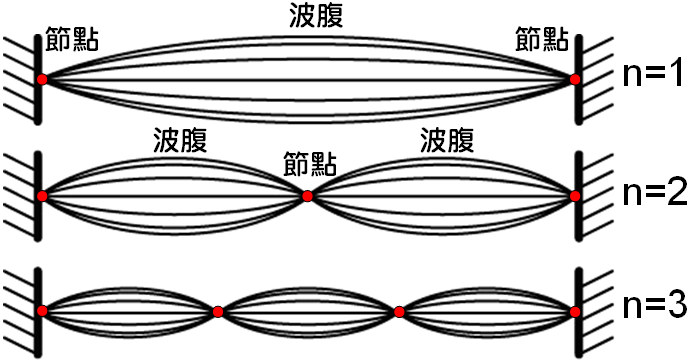
\includegraphics[width=10cm, center]{stationary_wave.png}
\caption{駐波示意圖} \vskip 10 pt
\label{fig:stationary_wave1}
\end{figure}

\begin{figure}[H]
\centering
\graphicspath{{physics/}}
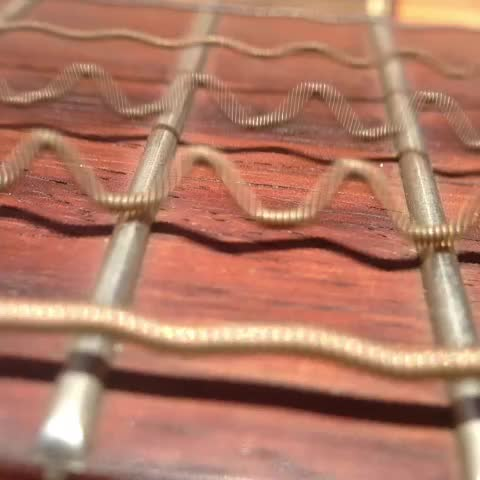
\includegraphics[width=7cm, center]{guitar.jpg}
\caption{吉他彈奏時,會產生駐波(肉眼通常不可見)} \vskip 10 pt
\label{fig:guitar}
\end{figure}

\item \textbf{波的干涉}:假設你有一隻鴨鴨,他在水面上漂浮著,他上下震盪產生週期性的水波向四方散去,現在,假設你有兩隻鴨鴨,假設這兩隻鴨鴨的震盪頻率一樣(即$\omega$一樣),兩隻鴨鴨個別產生的水波將會互相\textbf{干涉}成為下圖的情況。
\begin{figure}[H]
\centering
\graphicspath{{physics/}}
\includegraphics[width=\textwidth, center]{interfere.png}
\label{fig:interfere}
\end{figure}
\end{enumerate}


因為我們很難讓兩隻鴨鴨以完全相同的頻率震動,所以我們通常使用雙狹縫來進行這種干涉,因此這種現象被稱為\textbf{雙狹縫干涉},而且只需要一隻鴨鴨,把鴨鴨產生的水波用一塊板子擋住,並挖兩個很小的洞,則這個水波就會穿越這兩個小洞,產生一樣的現象。而且你可以發現,在打在裡面牆上的強度是條紋分布的,稱為\textbf{干涉條紋}。

為什麼會產生這種干涉條紋呢?因為水面上某一點到兩個波源的距離不同,會導致下列三種不同情況,$S_1$,$S_2$分別表示兩個波源。
\begin{figure}[H]
\centering
\graphicspath{{physics/}}
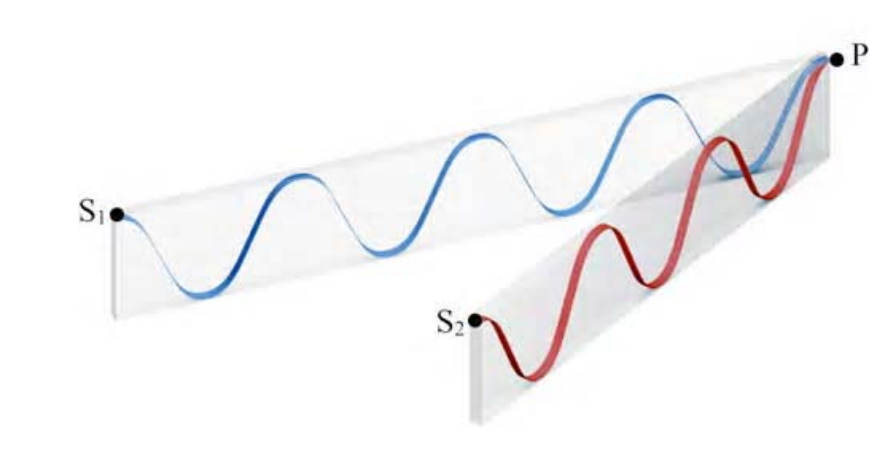
\includegraphics[width=7cm, center]{construct.png}
\caption{兩波峰重疊處,產生建設性干涉,能使其向上的合成位移更大} \vskip 10 pt
\label{fig:con1}
\end{figure}

\begin{figure}[H]
\centering
\graphicspath{{physics/}}
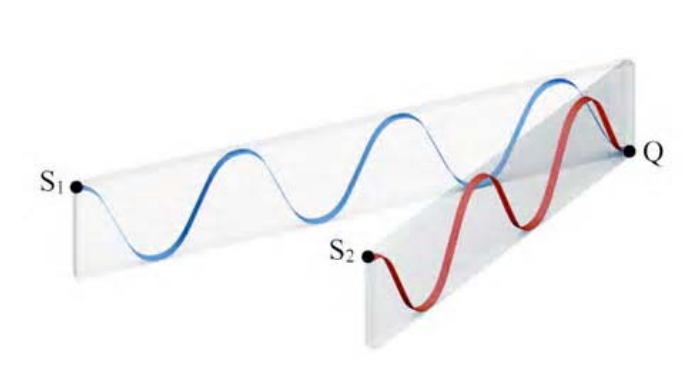
\includegraphics[width=7cm, center]{construct2.png}
\caption{兩波谷重疊處,也產生建設性干涉,能使其向下的合成位移更大} \vskip 10 pt
\label{fig:con2}
\end{figure}

\begin{figure}[H]
\centering
\graphicspath{{physics/}}
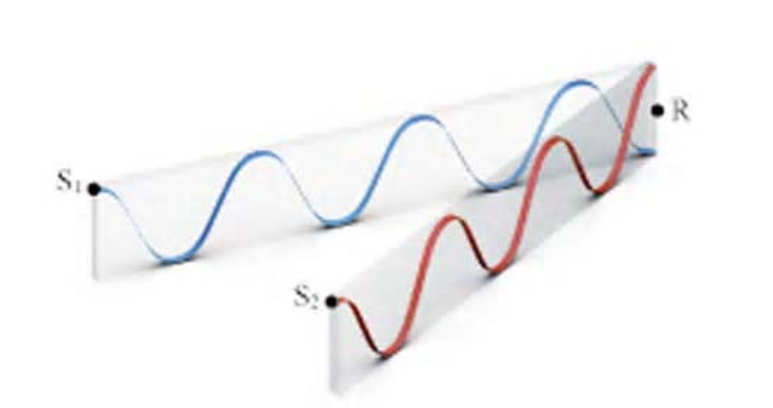
\includegraphics[width=7cm, center]{destruct.png}
\caption{波峰與波谷重疊處,產生破壞性干涉,能使其合成位移為零} \vskip 10 pt
\label{fig:de}
\end{figure}

{\Kai 【想想看,這三種情況會發生在上面那張水波圖的那些位置?(淺色的代表波峰、深色則代表波谷)】}





\section{附錄:利用坐標轉換概念推導偏移函數}


我們知道一個靜止的正弦波長這樣:$\sin⁡ \left (kx\right )$
若要讓他開始運動,則$x$的形式必須改變。

首先,想像這個波開始運行,但是杰穎站在這個波上,隨著這個波前進,設波速為$v$向著$x$軸正向運動,那麼這個人的速度也必定為$v$,杰穎因為什麼都有,所以他也有個以自己為圓點的坐標系$(x^{\prime}, y^{\prime})$,這個「$\prime$」表示他和站在地面上原本的靜止坐標系$(x,y)$是不同的坐標系。對於這個移動中的杰穎來說,因為他和波沒有相對運動,所以他看到的波是靜止的,他用他自己的坐標系描述的話就是
$$
y^{\prime}=\sin \left(\frac{2 \pi}{\lambda} x^{\prime}\right)
$$

因為$(x^{\prime}, y^{\prime})$這個坐標系相對於$(x,y)$往$x$軸正向進行運動,假設兩個在$t=0$的時候重合,那麼兩個坐標系之間就會滿足
$$
\begin{array}{c}{y=y^{\prime}} \\ {x^{\prime}=x-v t}\end{array}
$$
將杰穎坐標系轉換回地面的靜止坐標系,且使用$\frac{v}{\lambda}=\frac{1}{T}$
$$
y^{\prime}=\sin \left(\frac{2 \pi}{\lambda} x^{\prime}\right) \Rightarrow y=\sin \left[\frac{2 \pi}{\lambda}(x-v t)\right]=\sin \left(\frac{2 \pi}{\lambda} x-\frac{2 \pi}{\lambda} v t\right)=\sin \left(\frac{2 \pi}{\lambda} x-\frac{2 \pi}{T} t\right)
$$

定義$\frac{2\pi}{\lambda}\equiv k$ (波數)、$\frac{2\pi}{T} \equiv \omega$ (角速度),可以把公式整理成
$$
y=\sin (k x-\omega t)
$$

如果原始波函數為零的地方不在原點上,多一段距離則相當多一個相位角 $\phi_0$,則變為
$$
y=\sin \left(k x-\omega t+\phi_{0}\right)
$$

這個就稱為移動後的正弦波函數。

\chapter{從古典到近代量子物理}
\chapterauthor{丁安磊}
\setcounter{section}{-1}
\section{引言}
量子理論是近代的物理領域之一,量子物理的理論是非常難懂的,因為他的內容幾乎都與我們的直覺相牴觸,例如你有一定的機率可以穿牆,光波是粒子,電子是一種波,等等!不要那麼快趴下!這堂課會使用循序漸進的方式帶你探索物理的發展史,你們可以把他當作在看八點檔,時不時的會出現超展開的情節,請想像你就是那些科學家,跟隨著他們的腳步探索物理。(以下的歷史不保證完全正確)

如果以下的數學讓你感到頭昏,你可以忽略它,這不會影響到你的體驗,但有件事你必須謹記在心:數學公式與推導在物理學是不可或缺的,他展現了物理學的美妙和邏輯,因為數學能以最客觀和最精密的方式描述物理定律。

還有,科普與科研是完全不同的,科學雖然只能被少部分人研究,但科學能被大部分人欣賞,不能被大部分人欣賞的科學通常是沒有被研究好的科學。

現在讓我們進入時光機,回到西元前的時代,你現在在古希臘,辯士學派杜絕探究世界的真理,但希臘三大哲學家之一亞里斯多德思考著他的自然哲學。
\section{古希臘物理學(亞里斯多德物理學)}
從西元前300年左右,最早的物理學由古希臘哲學家亞里斯多德開創,由於亞里斯多德的地位,這些理論維持了將近兩千年都沒有被質疑,雖然它作為物理學的開端,但對於現在的我們來說,裡面有些理論看起來都很智障,舉幾個例子如下:
\begin{itemize}
\item \textbf{四元素理論}:亞里斯多德認為四種主要元素組成地球:土、氣、水及火,相信這個大家都聽過,對於現在的我們來說當然很唬爛。
\item \textbf{地球是宇宙的中心}:亞里斯多德認為宇宙萬物都繞著地球轉,從地球上看,不管是太陽、月亮、恆星,看起來都是繞著我們轉的。
\item \textbf{物體受力會做直線運動}:這對於沒學過\textbf{牛頓力學}的人來說看起來很合理?不過很遺憾,他是錯的。
\item \textbf{光線是從人的眼睛射出}:這顯然是錯的,它們可能是覺得夜晚中貓咪的眼睛會發光,所以這麼認為,不過貓咪很可愛這次我就原諒你吧。
\end{itemize}
亞里斯多德對於物理學的理解加上他的權威,建立起了看似屹立不搖的大樓,兩千年內沒有人能推倒這棟大樓,塑造了中世紀的學術思想,但直到牛頓這個叛亂份子居然輕鬆地用他的牛頓力學推倒了這棟大樓,並建立起了牛頓的經典力學體系,我們來看看這棟大樓的豆腐渣工程在哪:亞里斯多德雖然嘗試以理性來解釋大自然,但這些理論和現代科學比較起來,都有以下共通點:過於主觀、缺乏嚴謹證明。但我們還是要感謝亞里斯多德先生,作為先驅,你盡力了。

現在直接飛到牛頓那邊,來看看他做了什麼吧。


\section{古典物理學}
從中世紀開始的科學革命,帶給了科學突破性的進步,其中的\textbf{科學方法}的變革,帶給了引導著各門科學的發展,其中當然也包含物理學,物理學在這個時期逐漸壯大、統一,每個領域都逐漸的變成神聖而不可分割的一部分。注意,以下的理論是並立發展的,不是依照先後順序排列的。 
\section{古典物理學-牛頓力學}
牛頓寫了一本書《自然哲學的數學原理》,裡面使用嚴謹的數學來描述力學定律,他把物體的運動模式統合成三條牛頓運動定律。還有被蘋果砸到之後想到的萬有引力定律,表示兩物體之間的引力與他們的質量成正比,與他們之間的距離平方成反比。
\begin{figure}[H]
\centering
\graphicspath{{physics/}}
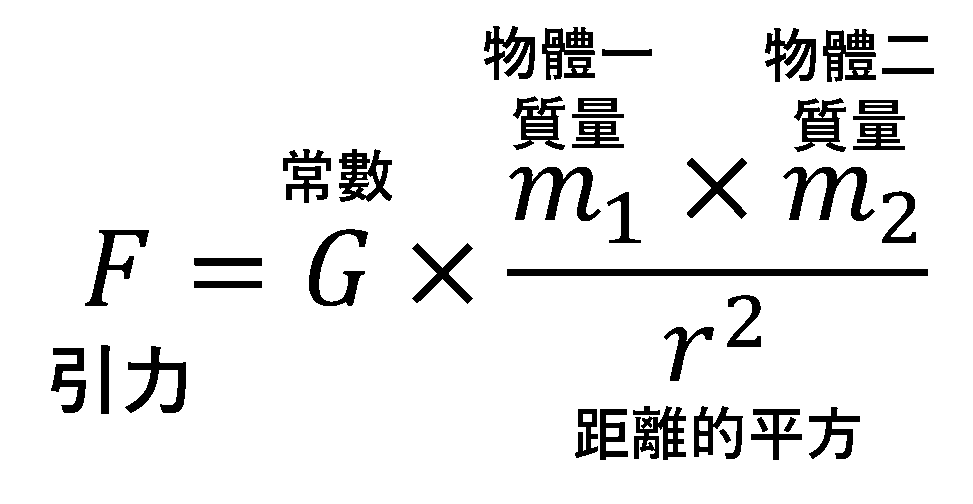
\includegraphics[width=5cm, center]{newton-law.png}
\caption{牛頓的萬有引力定律}
\label{fig:newton-law}
\end{figure}

\section{古典物理學-電磁學}
電學的方面,庫倫使用扭秤實驗得到了兩個帶電物體之間的電力
\begin{figure}[H]
\centering
\graphicspath{{physics/}}
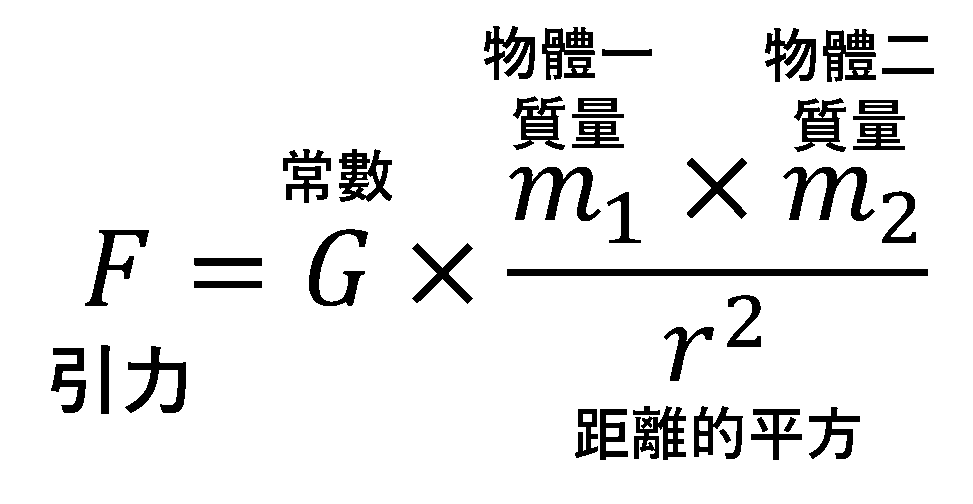
\includegraphics[width=5cm, center]{newton-law.png}
\caption{庫侖定律}
\label{fig:coulomb-law}
\end{figure}
有沒有覺得眼熟?他的形式就和重力的公式一樣!\\
磁力的形式比較複雜,但我們也能發現距離平方反比的特性
$$\Updelta B \propto \frac{I \Updelta L}{r^{2}}\mbox{;}F=q v B $$
\begingroup
\captionof{figure}{磁場的性質和磁力與磁場的關係(沒有解釋方向)}
\endgroup
\begin{tcolorbox}[breakable, title={專欄:平方反比定律}, before upper={\parindent2em}, parbox=false]

牛頓重力公式和庫倫定律都具有一樣的形式,我們可以發現他們的共同性質就是,力與距離的平方成反比,這是巧合嗎?我不這麼認為。我們以光線為例子來說明平方反比定律,假設杰穎想要拍一個燈泡(光源),他為了不讓照片曝光太亮或太暗,要如何調整光圈的大小?(光圈可以調整相機接受光線的面積大小)

我們可以將光想成許多條的光線平均向外擴散,我們假設光線不會因為傳播而變弱,所以如果我們在以光源為圓心的球殼上,不論半徑多大,接受到的光線數目是一樣多的。
\begin{figure}[H]
\centering
\graphicspath{{physics/}}
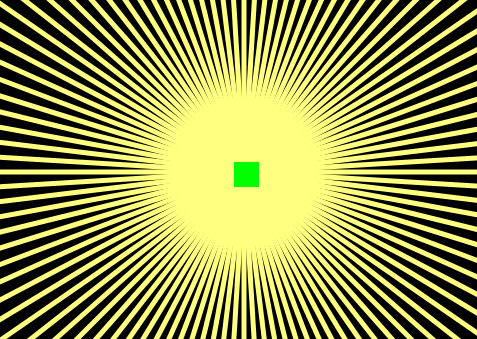
\includegraphics[width=5cm, center]{light.png}
\caption{光線散播圖}
\label{fig:light}
\end{figure}
當杰穎距離光源越遠,雖然光線一樣多,但他可以接收到的\textbf{光線密度}就會越小,也就是說,杰穎的光圈就需要張的更大,來接收足夠多的光線,下圖展示光圈的大小與距離的關係。
\begin{figure}[H]
\centering
\graphicspath{{physics/}}
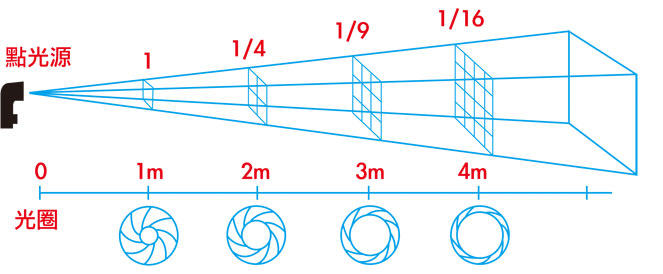
\includegraphics[width=7.5cm, center]{square-light.png}
\caption{平方反比定律的直觀理解}
\label{fig:light}
\end{figure}
在物理上,光線的密度定義為\textbf{照度},光線強度定義為\textbf{亮度},表示式為:
$$ \mbox{照度} = \frac{\mbox{亮度}}{r^2} $$

那麼,在力的部分,我們要如何思考平方反比定律呢?

我們引入力場的概念,重力場的大小定義如下,同樣與距離平方成反比,電力場擁有相同的情況

$$ \mbox{重力場 } g = \frac{GM}{r^2} \mbox{;電力場 }E=\frac{kQ}{r^2} $$

這裡以重力場為例,$M$代表建立這個場的質量的值,當有質量為$m$的物體位在這個場內,會施給他大小為場強$\times m$的重力,你可能會想說,為什麼我們要特地定義出一個場?原本的公式不是就可以描述重力的大小了嗎?

最初,會定義場的概念,是為了解釋\textbf{超距力}的作用,請思考一個問題,如果太陽瞬間消失了,地球會馬上飛出去嗎?答案是不會,我們必須考慮重力場傳播的速度,這個速度\textbf{就是光速},所以說,當太陽瞬間消失,等到過了8.3分鐘,地球將變為一片黑暗,並同時脫離軌道(因為太陽與地球的距離為1億5千萬公里,光速為每秒跑30萬公里,所以光與重力場從太陽傳播到地球的時間約為8.3分鐘),和光線密度一樣,我們可以把力場當成\textbf{力線密度},這也很好的解釋為什麼重力場會滿足平方反比定律。

電場的情況較複雜一些,因為電場的變化會產生磁場,反之亦然,以下將討論電場與磁場的關係。
\end{tcolorbox}

一開始,大家都覺得電與磁之間沒有關係,有人專門研究電學,有人專門研究磁學,直到一位大學教授厄斯特出於好奇心,將指南針放在流通著電流的線上,結果發現指南針的指針偏轉了!

接著,有許多人在研究電場與磁場之間的關係,如安培、法拉第等人,但最後被馬克士威統合成美妙的四條方程式。

$$ \nabla \cdot \mathbf{E}=\frac{\rho}{\varepsilon_{0}} $$
$$ \nabla \cdot \mathbf{B}=0 $$
$$ \nabla \times \mathbf{E}=-\frac{\partial \mathbf{B}}{\partial t} $$
$$ \nabla \times \mathbf{B}=\mu_{0} \mathbf{J}+\mu_{0} \varepsilon_{0} \frac{\partial \mathbf{E}}{\partial t} $$

\begingroup
\captionof{figure}{馬克士威電磁定律}
\endgroup

這四條方程式稱為馬克示威方程組【參閱附錄:\autoref{maxwell}】,我先給這方程組下一個評語:困難又簡單,難就難在他用了複雜的數學描述,簡單就簡單在他只用四條方程就描述了\textbf{大部分}電與磁的特性與關聯(注意是\textbf{大部分}) \par

你可能會想問,這是甚麼鬼?三角形是啥?為什麼那個長得像6的東西不能消掉?不用擔心,你不用懂這些計算,我只告訴你這些方程式告訴我們的結論:

\begin{itemize}
\item 第一條:其實他就是庫倫定律,只是物理學家喜歡把他寫成看起來一樣而且很酷的樣子,呵呵。
\item 第二條:它表示世界上不存在磁單極,甚麼意思?就是說我們不能只有N極和S極單獨存在,N極和S極一定會並存,不像電荷能夠有分開的正電荷和負電荷單獨存在,如果你把一個磁鐵分開,他會變成兩個磁鐵。
\item 第三條:他表示如果磁場發生變化,就會產生電場
\item 第四條:他表示如果電場發生變化、或有電流,就會產生磁場。
\end{itemize}

\begin{figure}[H]
\centering
\graphicspath{{physics/}}
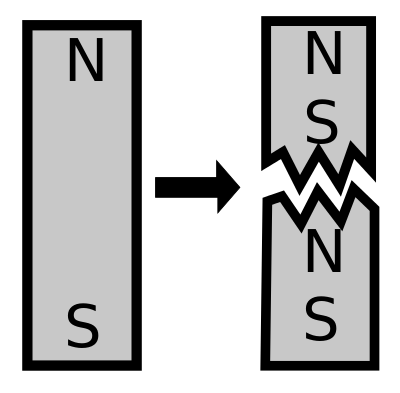
\includegraphics[width=5cm, center]{mag.png}
\caption{磁鐵分開後會變兩個磁鐵}
\label{fig:mag}
\end{figure}

當然,以上這些說法都是簡略到不能再簡略,要想真正搞懂你需要先學會向量、微積分、向量微積分(這東西和微積分簡直是天差地遠),如果你對這種困難的數學有興趣的話,請參閱附錄,也歡迎\textbf{來考武陵並加入物理讀書會(偷偷業配)}

如果你覺得沒興趣那也沒差,把結論收在心裡,我們繼續我們的旅程。

馬克士威利用他的電磁理論推論出\textbf{電磁波}的存在,細節推導很困難,不過你們可以這樣理解(雖然有點唬爛),第三條和第四條分別說電會生磁,磁會生電,所以如果當其中一個開始變化,就有可能會一直互相產生,並且他們震盪的\textbf{頻率決定這個電磁波在我們眼裡的顏色!}
\begin{figure}[H]
\centering
\graphicspath{{physics/}}
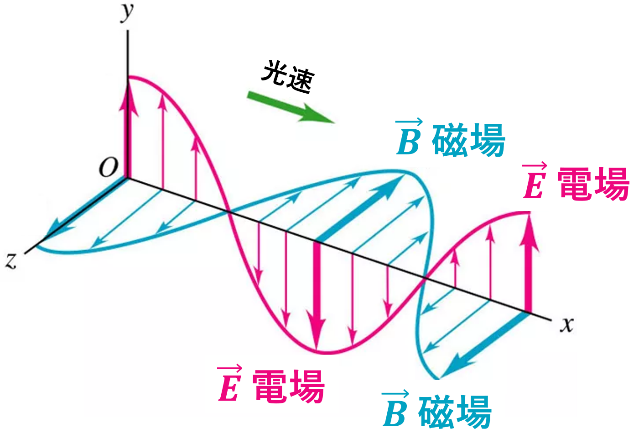
\includegraphics[width=7.5cm, center]{mag-wave.png}
\label{fig:mag-wave}
\end{figure}
二十多年後,赫茲在做放電實驗時,偶然發現身邊的一個線圈兩端發出電火花,原來是一個個小火花在迅速地來回跳躍。赫茲想到,這可能與電磁波有關。

後來,赫茲製作了一個十分簡單而又非常有效的電磁波探測器,這個探測器可以檢驗電磁波,赫茲把這個探測器放到電容旁邊,當電容的電壓足夠高,就會導通空氣,產生電火花,所以應該會產生電磁波,赫茲用諧振環接收電容產生的電磁波,諧振環中發出了電火花。所以,諧振環就好像收音機一樣,它是電磁波的接收器。就這樣,人們懷疑並期待已久的馬克士威電磁波理論終於被實驗證明了,此時風平浪靜的物理學貌似達到了巔峰,但他不知道這個實驗是個雙面刃,將帶給物理學一場腥風血雨的改革。

赫茲做實驗的時候,因為接收器的火花很小,幾乎看不到,他為了觀察清楚,把實驗室的燈關掉,而旁邊的發射器不斷的打出火花,也會對觀測接收器造成影響,於是他就找了一個塑膠箱子(塑膠1850年就被發明了),把他的接收器蓋住,然後在上面挖一個小洞,從小洞裡看接收器,或許這樣就能夠看得更清楚了吧?結果是,並沒有,用塑膠箱子蓋住之後,從接收器上看到的火花反而變得更微弱了。而且他還發現,如果拿高頻段的光例如紫光、紫外光,照著接收器,電火花會更容易出現。這個發現赫茲沒有做太多思考,但他不知道,他剛剛給繁榮的電磁理論埋下了一個伏筆,可惜的是,他在三十多歲的時候就過世了,無法看到接下來物理學的風起雲湧。
	
\section{古典物理學-熱力學}
熱力學研究溫度、壓力、體積、熱量、內能、熵等等物理量的關聯,你可以粗暴的把他當成研究熱的學科,這裡不多做贅述,就和竣程的化學課有點類似?
\section{古典物理學-光學}
終於要開始最有趣的部分了,光學的發展史可以比喻成物理大陸上最一場激烈的戰爭,持不同觀點的人們爭論著:光究竟是波還是粒子?我們再回去找這場戰爭的導火線:牛頓。

這裡插播一句話:人們總是傾向於巴著自己最了解的事物不放,因為已耗盡一生傾注全心全意於這些事物,不願放棄自己所堅信的事物,卻也失去了甚麼。請把這句話放在心裡,因為在物理學的發展上,這個情況不斷的出現。

心靈雞湯喝完,回到正題,時光機來到牛頓的小房間裡,這裡一片漆黑,忽然,一束白色光線打進來,散播成七種顏色的光,在屋內的牆壁上,出現了一條長長的彩色寬帶,牛頓看到了太陽的光能夠分散成七種顏色,於是他認為白光是七種顏色的光粒子的混合,三稜鏡會將這七種顏色的粒子分開,他把他的研究成果交給英國皇家學院的一個三人的評議會。

三人中的一個人,名叫虎克,對,就是那個玩彈簧的虎克,也是那個觀察到細胞的虎克,虎克認為光是一種波,他是光波動學派的大將之一,光波動學派的創始人叫做格里馬第,格里馬第發現了光的繞射現象,我們知道水波也會發生繞射,所以他合理的推斷光會是一種波,虎克受到格里馬第的影響,他認為光是一種類似於彈簧波的縱波,所以當他看到牛頓的研究成果時,虎克對他的觀點做了非常嚴厲的批評,這下不得了,虎克顯然是沒有達爾的探測鏡,他不知道自己眼前的這個牛頓,戰鬥力超過9000!牛頓從沒見過有人這樣批評他,馬上爆氣花四個月寫出一篇長文砲轟虎克,虎克被嚇得暫時收斂,這場第一次波粒戰爭就此結束。

等等!還沒結束,這時,惠更斯加入了戰局,他在歐洲大陸上全力發展光的波動說,繼承了虎克的思想,引入了波前的概念,他用了自己的理論推導出了光波的反射和折射定律,後來甚至能夠拿來解釋方解石(某種碳酸鈣的結構)的雙折射現象,甚至是自己的對手牛頓發現的牛頓環現象,也被惠更斯的理論所解釋。不過很遺憾,惠更斯帶給光波動學派的興盛是暫時的,你眼睛業障重,因為牛頓站在波動學派的後面,他非常火,牛頓對虎克的仇恨久久無法散去,只要英國皇家學會有虎克的存在他就絕不踏進那裡一步。

等到惠更斯、虎克相繼過世,牛頓當選為英國皇家學會的主席,這時候的牛頓已經不是當年的那個牛頓了,他現在是寫了《自然哲學的數學原理》的牛頓,發明了微積分的牛頓,身為國會議員、造幣局局長的牛頓,牛主席在光粒人民共和國稱帝的第一步已經開始,他出版的《光學》用粒子說證明了色彩疊合、分散、薄膜透光、牛頓環、繞射、雙折射(細節不多做贅述),對光波動學派造成可觀的打擊,波動學派沒有了他們的領袖,它們自己內部也沒有個完善的理論,\sout{經常在立法院打架},終究難逃被統一的命運,終於,一道光線,各自表述的呈現了一面倒的情況,第一次波粒戰爭,由光粒子學派勝利。

轉瞬之間,一個世紀過去了,光粒子的觀念烙印於人們的思想中,但在這時,英國出現了一位甚麼都會的全才,叫做楊(Young),不是很年輕的那個Young喔,有些人也就叫他楊格包括我,這時你的英文老師可能會爆氣,因為ng裡面的g不發音,她會請你去把一篇作文重寫七次。總之,這個楊格呢是個甚麼都會的人,就像我們班的電神杰穎(編按:並沒有),什麼都知道,楊格被譽為「世界上最後一個什麼都知道的人」,他在13歲時,已經會說希臘文、拉丁文、希伯來文、義大利文與法文,楊格後來成為了一位醫生,楊格遇到的病人中,許多人都在跟他抱怨視力逐漸模糊的問題,那個時候近視的人就等於全盲了,於是楊格開始了他對光學的研究,想要治療這些人,最初,楊格研究牛頓環現象時,發現這種明暗相間的條紋可以用波的干涉來解釋,他也用他的干涉理論證明出了繞射的現象,也設計了一個非常經典的實驗來加強他的理論-光的雙狹縫干涉實驗。
	
	這個實驗的方法是,在面板後面放一個點光源,並且在面板上鑽出兩個非常狹窄的縫隙(雙狹縫),並觀察面板前面的牆壁上的亮度,如果牛頓的粒子說是對的,實驗的結果可能會是中間最亮,而越遠離中間則越暗【如圖\ref{fig:exp1}】,但楊格做出來的結果【如圖\ref{fig:exp2}】所示,產生了和水波一樣的干涉條紋!但這時候大家都沉浸在牛頓的美好世界裡,楊格的論文無處發表,他只好把他印成小冊子在路邊兜售,結果也只賣出一本。

\begin{figure}[H]
\centering
\begin{minipage}{0.5\textwidth}
\graphicspath{{physics/}}
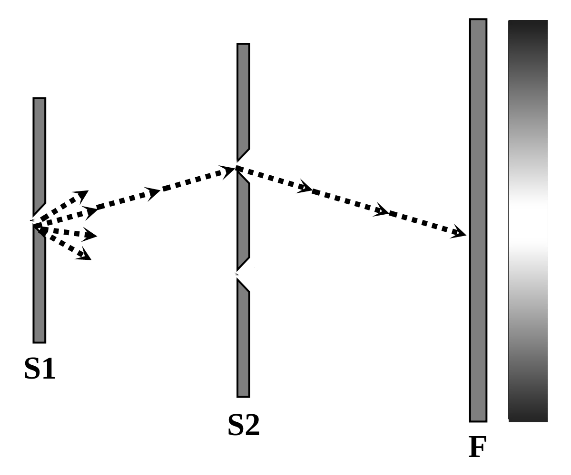
\includegraphics[width=\linewidth, center]{exp1.png}
\caption{粒子說預測的結果}
\label{fig:exp1}
\end{minipage}%
\begin{minipage}{0.5\textwidth}
\centering
\graphicspath{{physics/}}
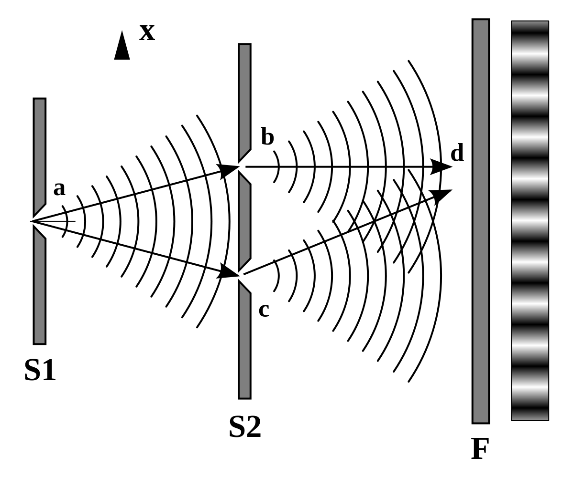
\includegraphics[width=\linewidth, center]{exp2.png}
\caption{楊格的實驗結果}
\label{fig:exp2}
\end{minipage}
\end{figure}

但是微粒派馬上開始發現,這次的對手實力不容小覷!微粒說無力反駁楊格的實驗結果,因為不管光粒子怎樣飛,都不會有兩個粒子碰在一起變暗的情況發生,微粒說為了反駁,派出了馬呂思,他使用技能「光的偏振現象」!這時光的波動說無法解釋他所發現的光偏振現象,第二次波粒戰爭開打,戰況又陷入膠著。

決勝時刻到來了,法國科學院(簡稱法科),公布了一道懸賞題目,內容是用精密的實驗與理論來確定光的繞射現象,法科的許多評委都是支持微粒說的人,他們的本意可能是希望有人能夠用微粒說來說明光的繞射。這時有個耍白目的人提交了一篇論文,他叫做菲涅爾,他使用光的波動觀點嚴密的推導出了光的繞射問題,他的推導過程天衣無縫,(你可能會問說,楊格不是已經用波動推導過繞射了嗎?很遺憾,根本沒人知道,包括菲涅爾。)但是法科的評委之一-帕松,發現菲涅爾的理論應用在圓盤的繞射上的時候,會在圓盤的中心出現一個亮點!你拿光照一個圓盤,中心會出現一個亮點?帕松覺得這真是笑死人了,帕松給了菲涅爾的理論一巴掌,但是法科的評委之一,阿拉果,又帶給波動派一個超展開,他堅持要給帕松發現的亮班做一個實驗,帕松本人則認為這個現象荒謬至極到不必做實驗來驗證,就在帕松認為自己又一次帶領微粒派擊退波動派的同時,阿拉果照出了那個亮點!戰況大逆轉!菲涅爾的理論大獲全勝,而最搞笑的事,這個圓盤繞射產生的亮斑明明是帕松否認的現象,結果被命名為帕松亮斑,真是物理史上的一大羞辱。

\begin{figure}[H]
\centering
\graphicspath{{physics/}}
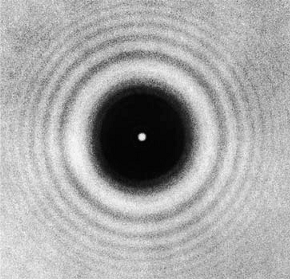
\includegraphics[width=7.5cm, center]{arago.png}
\caption{帕松亮斑}
\label{fig:mag}
\end{figure}

其後波動學派對於粒子學派的反攻毫不留情。第一波進攻,為了解決馬呂斯的偏振問題,菲涅爾假設光是一種橫波,而不是他們以前認為的那種縱波,被打敗的馬呂斯只好回到他的悲慘世界(沒人懂梗好嗎)。

再來,第二波進攻,說到這裡,我們來回憶一下牛頓是如何證明光的折射定律的,當光線從低密度的介質進入到高密度的介質,比如說從空氣進入到水或是玻璃好了,牛頓認為當光線在空氣中運行時,因為四周的萬有引力都一樣,所以光線會直線前進,但是當光運行到空氣與水之間時,一邊是空氣的萬有引力,一邊是水的萬有引力,因為水的密度更高,所以水的萬有引力比空氣更強,於是造成光在空氣與水之間被往水的方向拉動,所以對於粒子說而言,因為跑到水裡會被拉一下,光在水中的速度應該要更快才對。

第二波進攻是傅科和斐索的實驗,這時候科學的技術已經能夠測量光速了,於是他們著手測量光在空氣與水中運行的速度,這個實驗結果一旦出來,就決定了最終的勝利,結果出來了!光速在水中運行的速度只有空氣中速度的四分之三!光速在水中運行的速度只有空氣中速度的四分之三!

第三波進攻帶領波動的軍隊迎向完全的勝利,這次軍隊的將領-馬克士威,使用他的理論預測出電磁波的存在,並且計算出電磁波的速度,就等於光速!波動派終於反攻大陸,波動主義,統一光學,讓稱帝了一百多年的牛頓理論下台。

\section{黑體輻射}
不論是科普教材,還是大學課本,要介紹量子物理時都會提到黑體輻射,其實黑體輻射這個概念聽起來好像很難,但其實他就在你我身邊,因為只要溫度高於絕對零度,物質的粒子就一定會有震盪,根據馬克士威的電磁學理論,只要帶電粒子加速就會產生輻射,如果你聽不懂,你只要知道所有物體都會產生輻射電磁波就對了。
\begin{tcolorbox}[breakable, title={專欄:輻射函數圖}, before upper={\parindent2em}, parbox=false]

所有物體都會輻射?那為什麼我們看不到呢?因為溫度太低的物理的輻射都是紅外線,像是人體(37°C)輻射出的電磁波是紅外線,肉眼是看不到的,但當溫度逐漸升高,像是燒紅的木炭、鐵塊等等,因為粒子震動變得更厲害了,導致輻射出的電磁波頻率越大。某些物質甚至可以燒到變藍色、紫色、甚至到散發出紫外線!

我們知道,物體會輻射出電磁波,但因為物體內的帶電粒子不一定會有相同的震動頻率,所以這個物體內的帶電粒子可能會有各種的震動頻率,進而導致物體發出的電磁波也會有各種頻率的喔。右圖中的許多曲線代表不同溫度所輻射出的各種頻率電磁波的強度,如果還是覺得不太理解,先嘗試關注其中一條曲線,像是T=4000(T是溫度),我們可以發現在這個溫度下,物體輻射出最多的電磁波頻率在紅外線的部分,而在T=8000最多的是黃綠色的光(雖然你們看不到)

\begin{figure}[H]
\centering
\graphicspath{{physics/}}
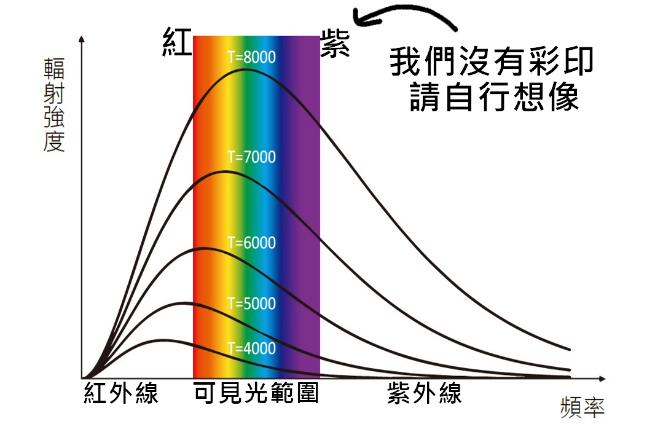
\includegraphics[width=7.5cm, center]{radiation.png}
\label{fig:rad}
\end{figure}
\end{tcolorbox}

黑體(Blackbody)是甚麼?我們知道物體會吸收、反射、輻射光線,黑體是一個物理學家想像出來的物體,我們稱為理想黑體,物理學家就是這麼任性,他只會吸收、輻射光線,而不會反射,但現實世界其實還是有能夠近似理想黑體的東西,例如太陽就很逼近一個理想黑體,你可能想說太陽明明一點都不黑啊?嗯…其實物理學家取名字也很任性。

古典物理學的研究過程大致如下:(1)發現某個現象(2)做實驗找出這個現象的數據(3)研究理論並推導出與實驗數據相符的結果。好了,現在你有一個黑體的模型了,他不會反射,就是這麼簡單,物理學家開始做實驗,找出黑體輻射的函數圖(上面那個),接著進到最後一步,使用各種理論推導出實驗的結果!首先第一位上場的是維恩,奮筆疾書,揮舞著他的鋼筆,使用寫出了維恩公式,把它的函數圖畫到紙上,高頻段的曲線和實驗數據很符合!但眼神往圖紙的左方一撇,低頻段的曲線居然與實驗數據有偏差!這不可能!一定是實驗誤差!但很遺憾,實驗是準確的,不管做幾次,曲線都長那樣。

後來有一個人叫做瑞立,他也來參與推導黑體輻射公式的工作,京士也來幫忙,他使用能量均分定理,推出了瑞立-京士公式。嗯,很棒,低頻段的曲線跟實驗數據一模一樣,但相似的場景再次上演,眼神往圖紙的右方一撇,居然飛出去了!這是不可能的!這代表物體會輻射出無限大的高頻率電磁波!這被稱為紫外災變,意思是輻射在紫外線頻段放出的巨大能量。
\begin{figure}[H]
\centering
\graphicspath{{physics/}}
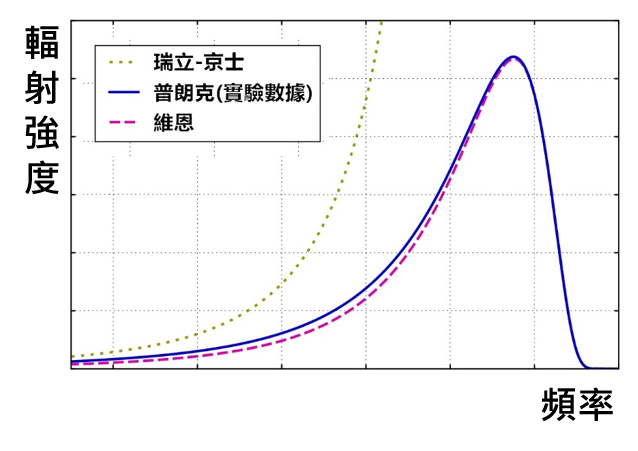
\includegraphics[width=5cm, center]{ultraviolet-catastrophe.png}
\label{fig:ultraviolet-catastrophe}
\end{figure}
其實在維恩推出他的公式之後,一位科學家普朗克也來對黑體輻射公式進行推導,他發現一項驚人的事實,他改變維恩的假設,加入「能量不連續」的假設,居然推出了和實驗數據一模一樣的數據!但這個「能量不連續」是什麼意思?他代表物體放出的輻射能量不是連續的,會有一個最小單位的能量,稱為\textbf{能量子}(energy quanta),而且這個最小單位的能量還正比於輻射電磁波的頻率,我這裡我寫下影響整個量子物理的公式。
$$E_{\mbox{最小單位}} = hf$$
直接這樣講感覺有點難懂,我們來做一些比喻,假設電磁波要把輻射能量帶出去的,把電磁波想像成攜帶能量包的人,但他每次只能拿幾包而已,沒有人再拿半包或0.9487包的,這稱為\textbf{能量量子化}。

\section{光電效應}
幾年後,愛因斯坦一邊發表狹義相對論,一邊研究光電效應問題,什麼是光電效應,還記得赫茲當年做得實驗嗎?如果有高頻率的光在照著發射器,更容易被打出電火花。其後有許多科學家投入相關的實驗,這些人的研究有一個結論,如果在乾淨的鋅金屬的表面(沒有會隔絕鋅金屬的氧化鋅),拿紫外線或紫光持續照射,會變成帶正電荷,合理推斷是表面帶負電的電子飛走了;但是如果拿紅外線或紅光照,不管拿多強的光,或是照多久的光,他都不會帶正電荷。

觀察敏銳的同學可能已經發現了,光電效應和古典電磁學是不協調的!為什麼?

電磁學認為,光是一種電磁波,他的強度(振幅)代表了他的能量,如果增強強度或增加照射的時間應該能夠打出更多、更高能量的電子。不過光電效應卻表明,只要你的電磁波頻率低於某個低限頻率,是無法打出任何電子的,但當頻率高於這個\textbf{低限頻率},隨便打都能打出電子,並且如果在這時候把強度增加,每個電子飛出來所帶有的動能,都是一樣的,只是飛出來的電子數增多了而已。

愛因斯坦也同樣受到這個問題的苦惱,他思考著:「提高頻率才能打出電子,……,提高頻率,提高頻率,提高頻率!?」他靈光一閃,燈泡忽然出現在他的頭上,他想到了普朗克的能量子,「嗯…,按照普朗克的說法,光的能量在空間中應該也不是連續的吧,而是由一些數目的能量子所組成的,好!就叫他光量子吧!」

後人把愛因斯坦的光量子(light quanta)稱作光子(photon)。

從愛因斯坦假設的光量子出發,一切都變簡單了,頻率更高的光線比如紫光、紫外光,根據普朗克的理論,會擁有更大的能量,因此當紫外光子作用到金屬表面時,就能激發出更高動能的電子,但是低頻的光,他的光子的能量太低了,沒辦法把電子激發出去,有些人可能會有問題:那為什麼不能讓很多的光子合作打出一個電子呢?這裡有個不太精確的解釋,但能夠說服你,當第一個光子將電子激發,一旦他沒有完全脫離,他會在非常短的瞬間掉回去,所以第二個前來的光子無法和第一個合作。

\begin{figure}[H]
\centering
\graphicspath{{physics/}}
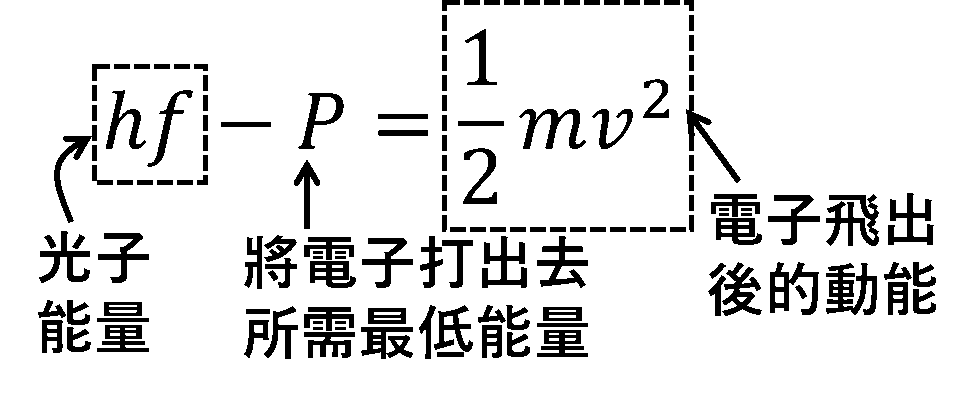
\includegraphics[width=5cm, center]{photon.png}
\label{fig:photon}
\end{figure}

這裡引用《量子物理史話》裡面的解釋(不瞞你說,前面蠻多也是參考來的)

{\Kai 我們把光電效應想像成一場有著高昂入場費的拍賣。每個光子是一個顧客,它所攜帶的能量相當於一個人擁有的資金。要進入拍賣現場,每個人必須先繳納一定數量的入場費,而在會場內,一個人只能買一件物品。}

{\Kai 一個光量子打擊到金屬表面的時候,如果它帶的錢足夠(能量足夠高),它便有資格進入拍賣現場(能夠打擊出電子來)。至於它能夠買到多好的物品(激發出多高能量的電子),那要取決於它付了入場費後還剩下多少錢(剩餘多少能量)。頻率越高,代表了一個人的錢越多,像紫外線這樣的大款,可以在輕易付清入場費後還買的起非常貴的貨物,而頻率低一點的光線就沒那麼闊綽了。}

{\Kai 但是,一個人有多少資金,這和一個“代表團”能夠買到多少物品是沒有關係的。能夠買到多少數量的東西,這只和“代表團”的人數有關係(光的強度),而和每一個人有多少錢(光的頻率)沒關係。如果我有一個500人的代表團,每個人都有足夠的錢入場,那麼我就能買到500樣貨品回來,而你一個人再有錢,你也只能買一樣東西(因為一個人只能買一樣物品,規矩就是這樣的)。至於買到的東西有多好,那是另一回事情。話又說回來,假如你一個代表團裡每個人的錢太少,以致付不起入場費,那哪怕你人數再多,也是一樣東西都買不到的,因為規矩是你只能以個人的身份入場,沒有連續性和積累性,大家的錢不能湊在一起用。}
\section{原子結構}
說完了黑體輻射與光電效應,來說說古典物理碰到的另一個問題:原子的結構。因為這在國二理化是一個章節,這裡為了節省篇幅,就不講得太細了。

科學家們所提出的原子模型發展如下。
\begin{enumerate}
\item \textbf{道爾頓原子模型}:道爾頓認為物體的最小基本單位是原子,無法再細分
\item \textbf{湯木生葡萄乾布丁模型}:J.J.湯木生發現了電子,但原子是電中性的,所以他認為原子內是數量一樣的電子和不知道是甚麼的正電荷鑲嵌在一起而成,他覺得整個原子可能有一個大區域的正電荷布丁,幾個電子在上面跑,看起來葡萄乾(?)
\item \textbf{拉塞福行星軌道模型}:因為他的α粒子散射實驗,他認為正電荷是集中在中心的小區域內,稱為原子核,電子以一個軌道繞著原子核運轉,就像行星繞著恆星轉一般。
\end{enumerate}
國中有講的原子模型大概就這三個,後面什麼中子之類的東西我就不多討論了,但其實原子模型的發展還沒有結束,為什麼,因為拉塞福的模型有個致命的錯誤,根據馬克士威的電磁理論,當電子運行在軌道上做等速圓周運動,就必定有個向心加速度,有加速度就會輻射出能量,那這樣電子就會不斷耗散能量直到墜落到原子核!個屁啦!怎可能,以上這些如果是真的將會在不到一秒鐘內發生,但我們現在還不是活的好好的,所以這個模型一定是錯的……嗎?

好了,先平復一下情緒,跟著拉塞福的學生-波耳一起來想這個問題。

有一天拉塞福要求波耳幫忙思考這個理論的穩定性問題,波耳思考著:「對於這個問題來說,要嘛老師的行星模型是錯的,要嘛馬克士威的電磁理論是錯的,只能二擇一」
	
「不管馬克士威的電磁理論有多麼的簡潔美妙,現在沒有人真正的驗證在原子的微觀尺度的電磁理論是否正確,我寧可拋棄馬克士威,因為老師的模型有α粒子散射實驗佐證啊!」

波耳的這一步,是即將帶給物理學大革新的一大步。
\section{氫原子光譜}
我們剛剛提到了牛頓的色散實驗,後來也有許多人跟進,在十九世紀初,人們用更精細的方法研究太陽的光譜,發現太陽的光譜中間居然有許多的黑線,代表在這個頻率上沒有光,人們一直不知道這些黑線是怎麼來的。

後來有人沒事幹,開始燒這個燒那個,結果發現某些氣體的光頻率居然和這些黑線的頻率一樣是一條一條不連續的,於是大家開始研究單原子氣體的吸收和發射光譜,各種不同的元素對應到不同的光譜線,舉最簡單的氫原子光譜線的波長為例:656,484,434,410,397,388,383,380,…奈米,大家都不知道這些光譜線的數學式要怎麼寫,但之後一位名叫巴耳末的數學老師,「猜」出了他的公式,把他的公式整理一下後變成
$$\frac{1}{f}=R\left(\frac{1}{2^{2}}-\frac{1}{n^{2}}\right)$$
其中$n$是正整數,$f$是氫原子能輻射出的光頻率,$R$是一個常數。

某天,波耳透過他的好朋友,得知了光譜的研究,所以他就發現這可以跟他的想法結合,波耳開始進行他的假設,並引用普朗克的量子理論把他用在自己的模型上,並且還把R算出來,結果和實驗數據測出來的R誤差非常小!但他還是沒有解決為什麼在微觀上電子不會掉進原子核的問題,但至少他是第一個用理論推導出光譜公式的人,於是他得了諾貝爾獎,哇喔,原來諾貝爾獎那麼好得喔?請別小看他,他雖然遇到了許多困難,但他還是為了物理學從古典進入到量子物理學的發展鋪了路。

\noindent
{\Kai 「這一理論還是十分初步的,許多基本問題還有待解決。」\\-波耳1922年諾貝爾物理學獎對自己的軌道理論的評論}

\section{德布羅意的電子}
德布羅意出身於貴族世家,他爺爺曾經是法國總理,且專門研究歷史,所以德布羅意一開始就受到爺爺的影響,在巴黎大學讀歷史,後來受到身為物理學家的哥哥影響,專而研究物理。

他在一戰結束後跑去大學找博士班物理教授-朗之萬,朗之萬看到地位這麼高的人跑來找他,也不太敢拒絕,就讓他來上課吧,德布羅意也學了一些當時的量子理論和相對論等等,幾年過去了,接近博士班的尾聲,因為畢業一定要寫個博士論文,正當他愁著博士論文沒啥好寫的時候,他看到了愛因斯坦的光電效應理論,愛因斯坦認為:原本我們認為是波的光,居然有粒子的性質,於是他突然有個大膽的想法,我們原本認為是粒子的電子,是不是也可能有波的性質呢?於是他的博士論文就誕生了,利用相對論的質能公式和普朗克的公式
$$
E=m c^{2} ; E=h f \Rightarrow f=\frac{m c^{2}}{h}
$$
寫出電子的波長公式(實際的推導並非這麼簡單)。
$$
\lambda=\frac{c}{f}=\frac{h}{p}
$$

這讓許多人感到奇怪,電子是一個波?當時六位博士論文評委中有三位說:「我覺得不行」,但在朗之萬把德布羅意的論文交給愛因斯坦過目後,愛因斯坦就說:「我覺得其實可以」,搞錯了,應該是「It’s interesting」,聽到愛因斯坦這麼說,評委回心轉意,於是他的博士論文就過了,耶!

常有人對於德布羅意的博士學位有意見,但他的這個預言將在物理史上流芳百世。

\begin{tcolorbox}[breakable, title={德布羅伊的博士論文和他的諾貝爾獎,出自《量子物理史話》}, before upper={\parindent2em}, parbox=false]

1925年4月,在美國紐約的貝爾電話實驗室,戴維森和革末在做一個有關電子的實驗。這個實驗的目的是什麼我們不得而知,但它牽涉到用一束電子流轟擊一塊金屬鎳。實驗要求金屬的表面絕對純淨,所以戴維森和革末把金屬放在一個真空的容器中,以確保沒有雜質混入其中。

不幸的是,發生了一件意外。這個真空容器因為某種原因發生了爆炸,空氣一擁而入,迅速地氧化了鎳的表面。戴維森和革末非常沮喪,不過他們並不因此放棄實驗,他們決定,重新淨化金屬表面,把實驗從頭來過。當時,去除氧化層的好辦法就是對金屬進行高熱加溫,這正是戴維森所做的。

容器裡的金屬,在高溫下發生了不知不覺的變化:原本它是由許許多多塊小晶體組成的,而在加熱之後,整塊鎳融合成了一塊大晶體。雖然在表面看來,兩者並沒有太大的不同,但是內部的劇變已經足夠改變物理學的歷史。

當電子通過鎳塊後,戴維森和革末瞠目結舌,久久說不出話來。他們看到了再熟悉不過的景象:X射線繞射圖案!可是並沒有X射線,只有電子,人們終於發現,在某種情況下,電子表現出如X射線般的純粹波動性質來。電子,無疑地是一種波。

因為這歷史性的發現,德布羅意得到1929年的諾貝爾物理學獎,很少有人能夠用博士論文獲得諾貝爾獎的,而且還是只有兩頁的論文。
\end{tcolorbox}

\section{薛丁格方程式}
任何型態的波都會有他的波方程,薛丁格認為如果電子是波,那麼他也會有一個屬於他的方程式,於是,他算出來了(怎麼算,不要問,你會怕)。
$$
-\frac{\hbar^{2}}{2 m} \frac{\partial^{2} \psi}{\partial x^{2}}+V \psi=i \hbar \frac{\partial \psi}{\partial t}
$$
其中你只要關心這個長的像三叉戟的希臘符號ψ,他叫做波函數,我們可以透過某些神奇魔法(同樣,不要問,你會怕)算出這個波函數,但是這個波方程可以解出很多種的波函數,而且你還可以透過更多神奇的方法找出這個波函數所對應的能量,太棒了!\footnote{其實波方程解出來的波函數不一定是一個波,他只是有可能解出來是一個波,他也可能是其他函數例如指數函數等等}

你發現我好像漏講了什麼,我已經預料到你會問這個了:什麼是波函數?…………嗯?快回答阿?你的心裡這樣想著,為什麼要一直玩精神分裂?這個人是不是想把講義灌水,在這邊放一堆幹話?痾,不對啊上面的東西已經多到爆了沒必要灌水,嗯……,為什麼呢?還是他根本就不知道波函數是甚麼?

哇,你猜對了,我真的不知道,順帶一提,薛丁格也不知道喔,他不管把任何東西代入波函數都失敗。

電子真的是像薛丁格想像的那樣是個\textbf{實體的波動}嗎?但是波函數會遍佈在空間內各個地方?可是我們從來沒有發現過這個波的任何一部分,電子只要現身,也就是\textbf{在我們觀察他的時候},他就一定是一個完整的物體。

\section{波函數的意義}
突然,這時有位物理學家玻恩出手了,他提出:「波函數的平方是機率」,這種說法受到了包含薛丁格在內的許多物理學家的反對,預測事務的發展情況是物理學的目的之一,現在你告訴我,物理學家連個電子下一秒會出現在哪裡也不知道?連一個電子也找不到,算什麼物理學家,但是接下來殘酷的事實告訴我們,玻恩的說法直到現在都和我們的實驗完全符合,等等,先別急著轉行學歷史!即使不能預測未來,物理還是很有趣的。

即使薛丁格本人並不能夠接受波函數代表一種機率波,但他自己也無法解釋什麼是波函數,物理學家還是逼不得已只能接受這個波函數沒有任何物理上的含意,僅僅代表這個電子在空間中某處被觀測到的機率。我們只能間接地從波函數求得各種物理過程發生的機率,而不能預測這個電子下一刻確切的位置。所以「波函數布滿空間」意義就是在空間中各點都有發現電子的機率。

我們知道波會有干涉的現象發生,所以如果依照玻恩的說法,薛丁格波動方程式預測電子在通過微細的雙狹縫後,電子的波函數會有高低起伏的干涉效應產生,這個實驗非常難做,因為電子非常小,所以這兩個縫必須要夠小才能夠形成干涉的圖樣,直到薛丁格方程式發表的40多年後,才有人做出電子的雙狹縫干涉實驗,總之你知道他是會發生的就好。

\begin{tcolorbox}[breakable, title={薛丁格方程原子模型}, before upper={\parindent2em}, parbox=false]

如果使用薛丁格方程式解出氫原子的電子機率分布,將會得到非常複雜的結果(如圖),如果要尋求他的物理意義,薛丁格方程裡面的V表示他的位能,這一項對方程式的解影響巨大,他會導致波函數被壓縮在原子附近的範圍內,這些波函數被壓縮起來的情況下就會自己與自己產生干涉,這些干涉的結果只有穩定的會留下來,剩下的就造成了我們看到的\textbf{電子軌域}。
\begin{figure}[H]
\centering
\graphicspath{{physics/}}
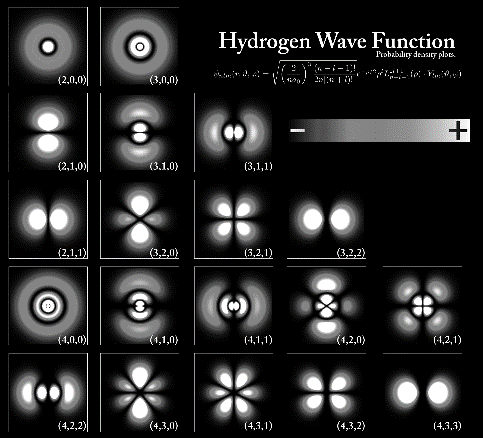
\includegraphics[width=\linewidth, center]{wave-function.png}
\label{fig:wave-function}
\end{figure}
有個比較好理解,但是被過度簡化的例子-環形駐波

把電子想成繞著核運行的波,我們剛剛有學到,最基本的穩定波是駐波,所以會穩定下來的電子波就是環形的駐波,而且駐波也有量子化的影子,故許多人講解波耳行星模型常引用這個說法,但其實波耳原本的解釋沒有提到。
\begin{figure}[H]
\centering
\graphicspath{{physics/}}
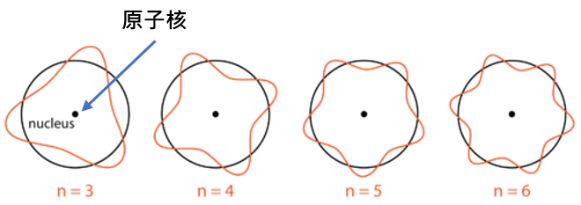
\includegraphics[width=\linewidth, center]{standing-wave.png}
\label{fig:standing-wave}
\end{figure}
\end{tcolorbox}
\section{奇怪的單粒子雙狹縫干涉}
\noindent
\begin{minipage}{0.7\linewidth}
\setlength{\parindent}{2em}
\setlength{\parskip}{1em}
\renewcommand{\baselinestretch}{1.1}
讓我們在來做個思維實驗,在自己腦海裡想像一個雙狹縫,我們再進行一次楊格的光的雙狹縫干涉實驗,但這一次,我們已經知道,光波的最基本單位是光子,一個光子的能量非常小,這代表每個光子必須要決定要穿過的是左邊的還是右邊的狹縫,而且光子已經是最小單位了,不能再分裂成一半然後在縫的後面合成。一般來說,我們發出的光裡面會有非常多的光子,所以從直覺上來看,只要有兩個以上的光子,出現干涉的條紋應該很正常,各個光子分別穿過不同狹縫,穿過狹縫後在狹縫的後方干涉形成條紋。

但是,如果只有一個光子呢?我們把光源的放出光的功率壓到非常低(後來真的有人做到了),所以光變成不是一大坨的光子一起穿越狹縫,而是一個一個的漫漫發射,這樣應該不會干涉了吧?因為它們都是自己一顆過去的。一開始,後方的屏幕很正常的出現了許多被光子打到形成的光點,幾顆幾顆的慢慢出現,一開始看起來是隨機分布的,但當時間過去,光點越來越多,我們發現光點的分布居然還是像原本的干涉條紋一樣!光點最多的地方對應到原本干涉條紋上的亮紋,反之亦然。

這個現象也發生在其他粒子身上,比如電子,如果電子發射器一次只發射一個電子,出現的分布情形也和干涉條紋一致!更誇張的是連巴克球(碳60)這種大分子也會出現干涉條紋。
為什麼會這樣?答案沒有人知道,但有許多量子力學詮釋試圖解答。
\end{minipage}%
\hfill%
\begin{minipage}{0.2\textwidth}
\begin{figure}[H]
\centering
\graphicspath{{physics/}}
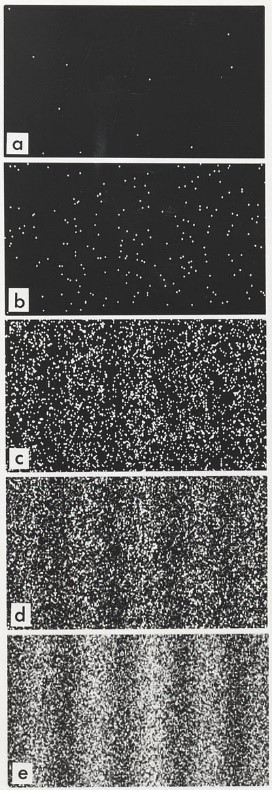
\includegraphics[width=\linewidth]{double-slit-exp.jpg}
\label{fig:double-slit-exp}
\end{figure}
\end{minipage}

\section{最多人相信的詮釋:哥本哈根詮釋}
由海森堡和玻恩等人的哥本哈根詮釋,因為它們都是哥本哈根大學研究量子力學的先驅,故得此名。

哥本哈根詮釋認為波函數沒有物理本質,是純粹的機率波,只有當他的位置\textbf{被觀察}的時候會出現\textbf{波函數崩塌},波函數本來是在空間中散播著,還沒被觀測時,他哪裡也不在,而且會出現波的干涉現象,但當你測量他的時候,他被迫要現身,這時候波函數會完全崩塌變成一個尖峰,這個尖峰就代表機率完全聚集在我們發現粒子的地方。而且重點是,這個波函數要崩塌在哪裡,完全取決於機率。

哥本哈根詮釋解決了我們的問題,卻也帶出了更多問題,像是為什麼觀測會讓波函數崩塌等等。其實,人們對量子力學還有更多詮釋,但其實不管它們怎麼解釋,都沒有人可以證明這些詮釋到底對不對,那麼,哪種詮釋比較好?其實沒人在乎,對於某些人,反正只要能算東西就好,他背後有什麼意義就留給想研究的人去研究吧,這也是\textbf{科學哲學}的研究對象之一,不過很多東西我也不懂,就沒有多做介紹了,只有簡報裡面稍微提到,想深入了解的話可以上網自己找資訊(感覺就沒人想知道)。

\section{不確定性原理}
由海森堡所提出的不確定性原理

\begin{center}
\noindent
{\Kai 一個運動粒子的位置和動量(質量乘以速度)不可被同時確定}
\end{center}

把這句話翻成更好理解的形式,他的意思是說,如果我們對粒子的位置進行測量,測量到的結果誤差越小,我們將無法確定他的動量是多少,反之亦然,如果測動量測得越準,我們就跟不能確定他的位置。
嗯,對於這段陳述,有些人可能會這樣理解。
當我們拿觀察電子等微觀粒子時,我們可能會需要拿光子去打他,但是測出電子的位置之後,光子可能會對他造成影響,造成動量的不確定。
\begin{figure}[H]
\centering
\graphicspath{{physics/}}
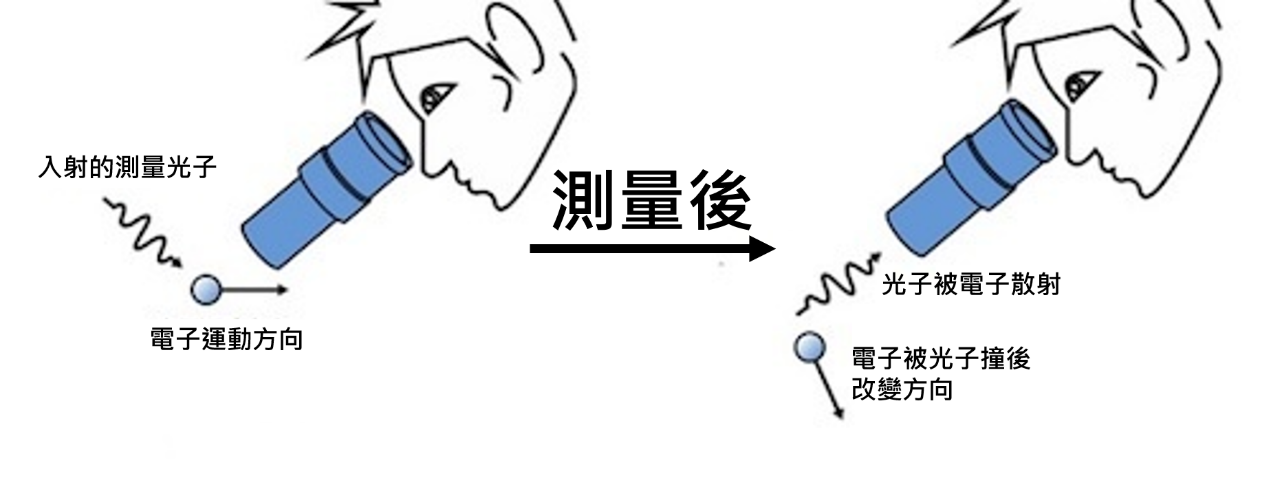
\includegraphics[width=\linewidth]{uncertainty-principle.png}
\label{fig:uncertainty-principle}
\end{figure}

照這個看法,不確定性是源於我們的測量儀器和技術不夠好?那如果我們真的找到一個更好的儀器或方法是不是就可以抹除不確定性?聽起來很合理?不過這其實是錯誤理解。

要進入量子力學的狀況,我們先來說說古典情況的不確定性。

假設你握著長繩的一端,有節奏的上下擺動產生一個波,如果有人問你,「這個波精確來說在哪裡?」,你沒辦法很好的回答,他分布在一個很寬的範圍,但如果有人問你「這個波的波長(頻率)是多少?」,你可以給出個合理的答案;反之,如果你快速的抖動一下繩子,將產生一個脈衝波,第一個問題(波在哪裡),就有很好的回答了,但第二個問題(波長是多少)卻又變得無法回答。這就是繩波的位置-頻率不確定性。
\begin{figure}[H]
\centering
\graphicspath{{physics/}}
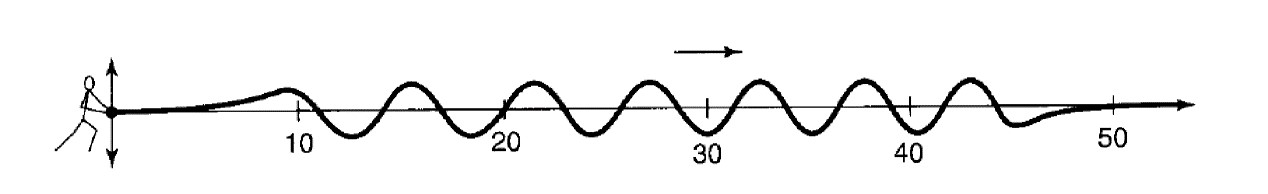
\includegraphics[width=\linewidth]{periodic-wave.jpg}
\caption{為週期波,頻率有很好的定義}
\label{fig:periodic-wave}
\end{figure}

\begin{figure}[H]
\centering
\graphicspath{{physics/}}
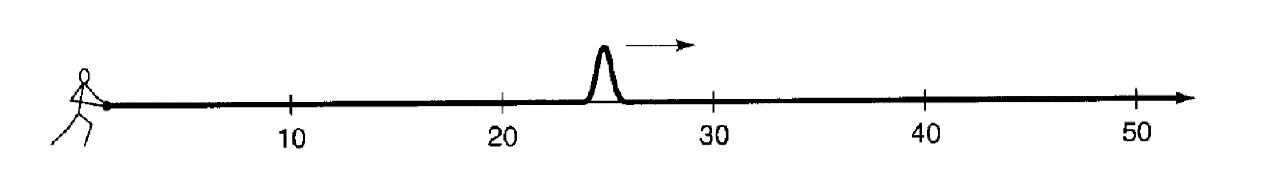
\includegraphics[width=\linewidth]{pulse-wave.jpg}
\caption{為為脈衝波,位置有很好的定義}
\label{fig:pulse-wave}
\end{figure}
回到量子的情況,德布羅意的物質波理論又說粒子的動量和波函數的頻率有關,所以古典的位置-頻率不確定性到量子世界中就變成位置-動量的不確定性。後人算出位置與動量的誤差滿足的關係(怎麼算出的又是另一個故事了)

$$
\Delta x \Delta p \geq \frac{h}{4 \pi}
$$

$\Delta x$表示位置的誤差,$\Delta p$表示動量的誤差,$h$表示普朗克常數,$\pi$是圓周率,你不必知道右邊的分數怎麼來的,你只要知道右邊的數非常小就好,所以當$\Delta x$越來越少,逼近於零,也就是位置的誤差越小,測量越精準,$\Delta p$就會暴增直到無限大,反之亦然。在巨觀的情況下,這個誤差小到可以忽略,但是對微觀物體來說就不能亂忽略了。

\section{結語} \label{justin-reflection}
看到這裡,相信許多人還是覺得頭昏腦脹(編按:我也是,排版好累,不過安磊真的很認真的在打這一章喔),但量子發展的一路走來是不可能用這堂課簡單帶過的!還有許多科學家的成就和發現都被省略了,以上都只是帶領你走馬看花,看見量子物理的奇妙之處,如果你瞥見了你中意的那朵花,那麼我的任務就達到了-「科學推廣」,接下來你要做甚麼都是你的事,你願不願意回去,自己踏過一遍量子的道路,拿著放大鏡好好的端詳那朵花;抑或是你認為物理和數學太難,不想深入研究,你們只要知道,眼前的這本講義,拿著這個講義的手,還有,你,都是很多的電子機率波在原子核周圍分布然後交互作用而已,卻能組合成這個複雜的世界,這也是他難以研究的原因,要是他好懂的話,可能我們就不存在了!
	
也請將要深入學習科學的同學謹記,我們不能讓每個人都參與科學研究的工作,但是其他人有權利知道這些研究的內容,請不要藏私,多和身邊對科學有誤解的人心平氣和的解釋而不是惱怒的否定。當你探索的越深,你一定會發現自己的無知,希望你會將這些疑惑轉化為動力,繼續追問,繼續探索下去。

\section{附錄:馬克士威方程式概述} \label{maxwell}
為了滿足想了解這四條方程式的同學,再把這些方程式做進一步的介紹,當然,想要完全搞懂你數學要夠好,若你覺得你數學夠好,請參閱\textbf{林琦焜:圖解梯度散度與旋度}(右方QR Code),或是遇到問題也可以找我。(這四條方程式沒有證明,因為我們發現他成正比而已)

\subsection{第一條:高斯定律\texorpdfstring{$\nabla \cdot \mathbf{E}=\frac{\rho}{\varepsilon_{0}}$}{TEXT}}
其中E表示空間中某個位置電場,$\rho$表示空間中某個位置的電荷密度,而$\nabla \cdot \mathbf{E}$表示$\mathbf{E}$在空間中的發散程度,因為電場是向量,你可以把他理解成\textbf{電場線},所以這條式子表示空間中某點電場線的發散程度,正比於空間中某點的電荷密度。事實上,將此式在球體區域積分後得到
$$
\int_{V} \nabla \cdot \mathbf{E} \mathrm{d} V=\int_{S} \mathbf{E} \cdot d \mathbf{A}=\frac{1}{\varepsilon_{0}} \int_{V} \rho \mathrm{d} V \Rightarrow 4 \pi r^{2} \mathbf{E}=\frac{Q_{e n c}}{\varepsilon_{0}}
$$

其實這就是庫倫定律,如果你努力的看還是不懂,我很難過,如果你看懂了,我更難過,我學了好久阿!!!

\subsection{第二條:高斯磁定律\texorpdfstring{$\nabla \cdot \mathbf{B}=0$}{TEXT}}
這條式子就像上面一樣,但是他永遠等於零,我們再回到第一條,如果有電荷密度,那麼電場的發散程度就不是零,如果沒有,那麼電場的發散程度就是零,所以這條式子就告訴我們,\textbf{沒有磁荷存在}(如果你能找到磁荷,恭喜你得諾貝爾獎)

\subsection{第三條:法拉第電磁感應定律\texorpdfstring{$\nabla \times \mathbf{E}=-\frac{\partial \mathbf{B}}{\partial t}$}{TEXT}}
積分後能夠把他變成一個比較好理解的形式
$$
\mathcal{E}=-\frac{d \Phi_{\mathrm{B}}}{d t}
$$

其中$\mathcal{E}$表示電動勢(就是電池的電壓), $\Phi_{\mathbf{B}}$表示磁通量,即磁場$\times$面積,所以這條式子就代表如果磁通量發生變化,就會產生一個電動勢。

\subsection{第四條:安培定律\texorpdfstring{$\nabla \times \mathbf{B}=\mu_{0} \mathbf{J}+\mu_{0} \varepsilon_{0} \frac{\partial \mathbf{E}}{\partial t}$}{TEXT}}
我們先忽略右邊的$\mu_{0} \varepsilon_{0} \frac{\partial \mathbf{E}}{\partial t}$的這一項,右邊的$\mathbf{J}$代表電流密度,左邊的$\nabla \times \mathbf{B}$表示磁場在某點旋轉的程度,所以這條式子代表若在這一點有電流,就會產生旋轉的磁場。

唬爛就到這裡,感覺有講跟沒有講一樣。

\section{講師介紹}
\begin{itemize}
\item 姓名:丁安磊
\item 性別:男
\item 特色:長得十分高壯,但不會打球(編按:聽說有時候體育課會偷跑回教室,根據本人說法是量子穿隧效應所導致)、十分有研究精神,常會研究某一些生物動力學問題到凌晨3、4點(編按:導致熊熊約講師出來看書時,約9點,講師通常都12點才來,抑或是直接不來了QQ)、對科技有興趣,有全班最酷的筆電Microsoft Surface、物理非常電、因為一直沒交講義,使熊熊十分惱怒。
\item 名言:喔我想到了,我們可以在科推加這個,一定超酷。(這些行為差點導致開天窗)
\end{itemize}

\part{生物}
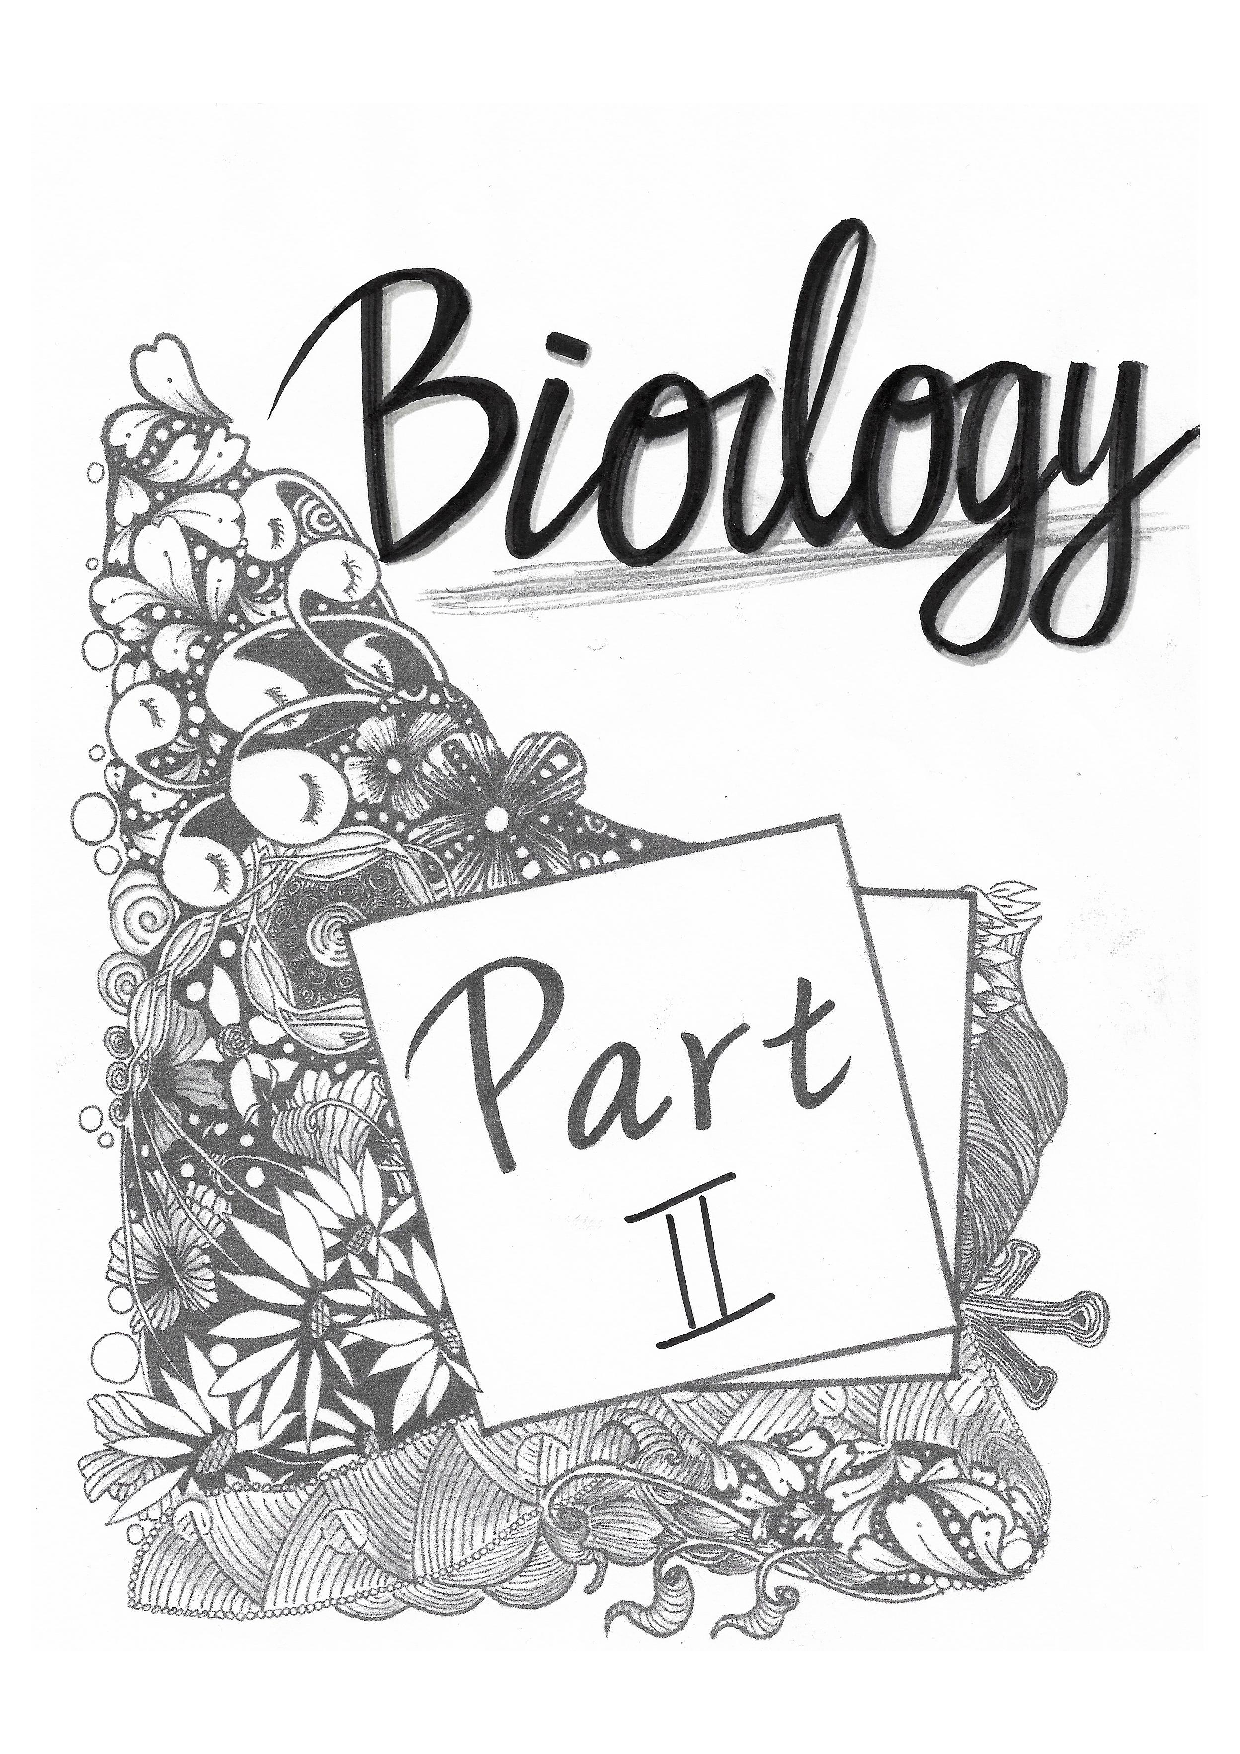
\includepdf[scale=0.9]{partImage/part2.pdf}
\chapter{免疫系統}
\chapterauthor{邱柏偉}

\section{摘要}
免疫系統(Immune System)為我們抵擋入侵的外來病原體(細菌和病毒),使我們免受於病痛的侵擾,現在就讓我們來看看免疫系統到底是怎麼運作的吧!!!
\section{免疫細胞的種類}
在我們的體內有一群專門負責抵抗病原體的細胞,它們就是白血球(leukocytes)。因此,接下來我們就來看看白血球又分為哪些種類吧!
\begin{enumerate}
\item 顆粒性白血球
	\begin{enumerate}
	\item 嗜中性球(Neutrophil Granulocytes):
		\begin{enumerate}
		\item 占人體內白血球約65\%~70\%
		\item 感染時做\underline{\hspace{2cm}},可\underline{\hspace{2cm}}病原體
		\end{enumerate}
	\item 嗜酸性球(Eosinophil Granulocytes):
		\begin{enumerate}
		\item 占人體內白血球約2\%~4\%
		\item 吞噬功能有限
		\item 發生過敏反應的時候,產生\underline{\hspace{2cm}}$\rightarrow$減輕過敏症狀
		\item 被寄生蟲感染時,嗜酸性球會附著在其表面,釋出破壞性酵素
		\end{enumerate}
	\item 嗜鹼性球(Basophil Granolucytes):
		\begin{enumerate}
		\item 占人體內白血球約<0.5\%
		\item 在特殊情形下會釋放出其內含的\underline{\hspace{2cm}}(Histamine)\\
		$\rightarrow$引起各種\underline{\hspace{2cm}}和使血管擴張(\underline{\hspace{2cm}})

		\end{enumerate}
	\end{enumerate}
\item 淋巴球(Lymphocytes):
	\begin{enumerate}
	\item T細胞(T Cells):
		\begin{enumerate}
		\item T細胞的表面有各種可以跟\underline{\hspace{2cm}}結合的專一性受體,能辨識不同
		\end{enumerate}
	\item B細胞(B Cells):
		\begin{enumerate}
		\item 能分泌\underline{\hspace{2cm}}(Antibody),又稱\underline{\hspace{2cm}}(Immunoglobin)
		\end{enumerate}
	\end{enumerate}

\end{enumerate}
\section{免疫反應}
用說的太麻煩了,我們來玩個遊戲來幫助我們了解免疫反應吧!

\section{講師介紹}
\begin{itemize}
\item 姓名:邱柏偉
\item 性別:男
\item 特色:在高一時參加生物奧林匹亞徵選,僅以一題之差落選,令人惋惜、每天都會帶著Campbell往返學校及家中(編按:Campbell為普通生物學的經典教材,精裝版一冊重達2公斤)、會對經過的熟人說小恐龍(編按:可試著對講師說小恐龍,可能會有驚喜喔)、最近為了貼補家用,兼職蜂農。
\item 名言:你是小恐龍、這題真的很小恐龍耶、小恐龍。
\end{itemize}

\begin{figure}[H]
\graphicspath{{biology/}}
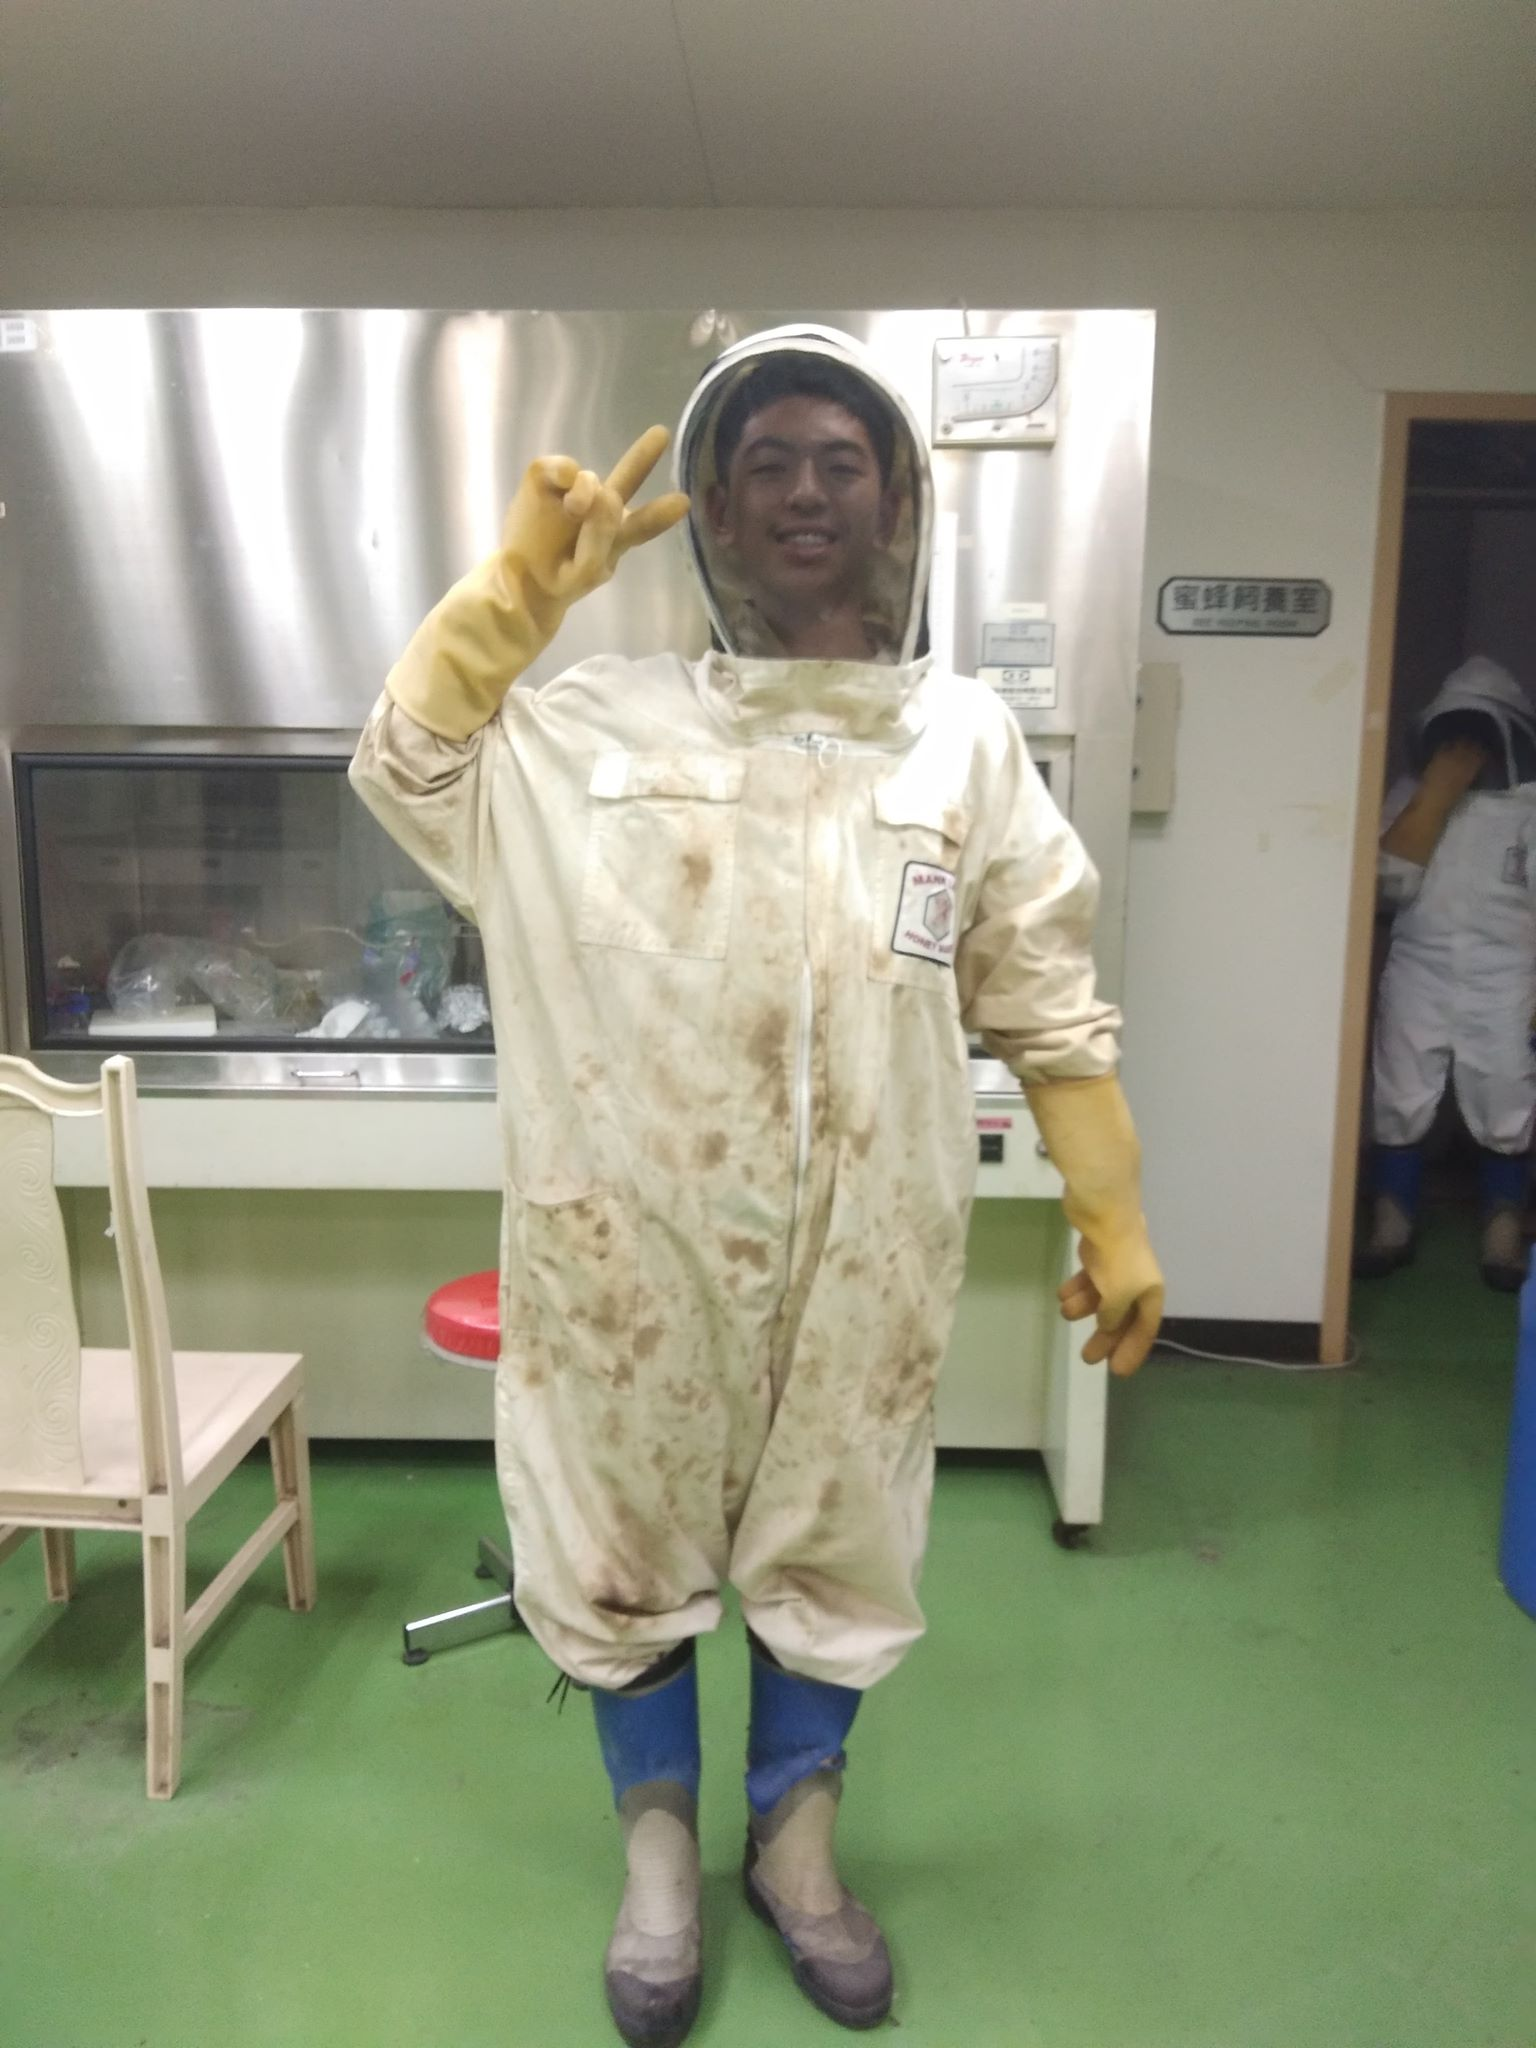
\includegraphics[width=8cm, center]{farmer.jpg}
\caption{蜂農} \vskip 10 pt
\label{fig:farmer}
\end{figure}
\chapter{物種想要起源但是物種不說}
\chapterauthor{高語儂}

\section{演化的定義}
地球上的生物,一直在改變。 \\
\subsection{複習下達爾文演化}
\begin{enumerate}
\item \textbf{變異:}
物種間,其性狀在個體存在差異
\item \textbf{過度繁殖:}
族群的個體數過多時,其生活所需的食物、水或空間便感不足。
\item \textbf{生存競爭:}
個體為了生存,彼此間會搶奪資源
\item \textbf{適者生存:}
成功的個體生存下來,並產生後代子孫。 
\end{enumerate}

\subsection{歷史小故事}
\begin{enumerate}
\item 達爾文在小獵犬之行後快30年(1859)才出版物種起源
\item 科學界在1870年代正式接受演化是事實。
\end{enumerate}

\section{演化的基本單位}
生物學將生命分成不同階層,從細胞、組織、器官到個體,並進一步形成族群、群集、生態系最後構成生物圈,那麼,\textbf{在研究演化時,科學家們通常會關注生命的哪個層面呢?why?}

事實上,演化可分為「微演化」和「巨演化」,今天我們要詳細介紹的是\underline{\hspace{6em}} 
微演化關注的是一個\underline{\hspace{4em}}中,等位基因頻率的變化。
巨演化通常指更大尺度的變化,例如新器官的生成,以及新物種的出現。

補充:微演化的分類
\begin{enumerate}
\item \textbf{天擇:}因為環境,而讓帶有特定「表型」的個體有生存優勢。
\item \textbf{基因漂變:}基因分布隨機的改變,例如:基因突變、瓶頸效應、創始者效應
\item \textbf{基因流動:}不同族群間的基因交換,例如:台灣人與日本人結婚
\end{enumerate}
\fbox{簡短名詞解釋}
\begin{enumerate}
\item \textbf{瓶頸效應:}\\
因為災難而使族群大量減少(例:洪水過後,整個地區只有一家人活下來,而他們剛好都有長高高基因,於是這個地區的基因就從有高有矮,變成100\%長高高基因了)
\item \textbf{創始者效應:}\\
族群中的一小部分獨立,開創新的族群(例:長高高家人移居到一個世外桃源,過了好幾代後,他們子孫的基因分布也會是長高高基因居多,而原本的舊族群卻是有高有矮)

\textbf{在已開發國家中,你覺得哪一種最常見?如果是未開發國家呢?}\\
\textbf{為什麼科學家要把演化分成這麼多類?}

\end{enumerate}

\section{天擇的方向}
會造成基因頻率頻率改變(aka微演化)的機制主要為三種:\textbf{天擇}、\textbf{基因漂變}、\textbf{基因流動}。 \\
我們都熟悉的是天擇。天擇偏好某些表現型,讓有生殖優勢的基因保存下來,那麼天擇有哪些偏好呢? \\
天擇分為:
\begin{enumerate}[label=(\alph*)]
\item \textbf{定向型天擇:}環境對某一種極端型的偏好,某特定型態的表型增加
\item \textbf{分裂型天擇:}對中間型表型不利,兩端極端的表型增加
\item \textbf{穩定型天擇:}比較極端的表型被剔除,最常見的中間型增加,群體\underline{\hspace{8em}}
\end{enumerate}
\fbox{試著分類以下的情況}

\noindent
( )細菌演化出抗藥性 \\
( )工業革命後,從黑白蝴蝶各半,變成以黑蝴蝶居多 \\
( )加拉巴哥群島上食物減少,能獵食特定食物的鳥增加;例如尖細長喙、或較大且厚的喙 \\
( )臺灣新生兒平均體重大多集中在3000~3300公克 \\
\begin{figure}[H]
\graphicspath{{biology/}}
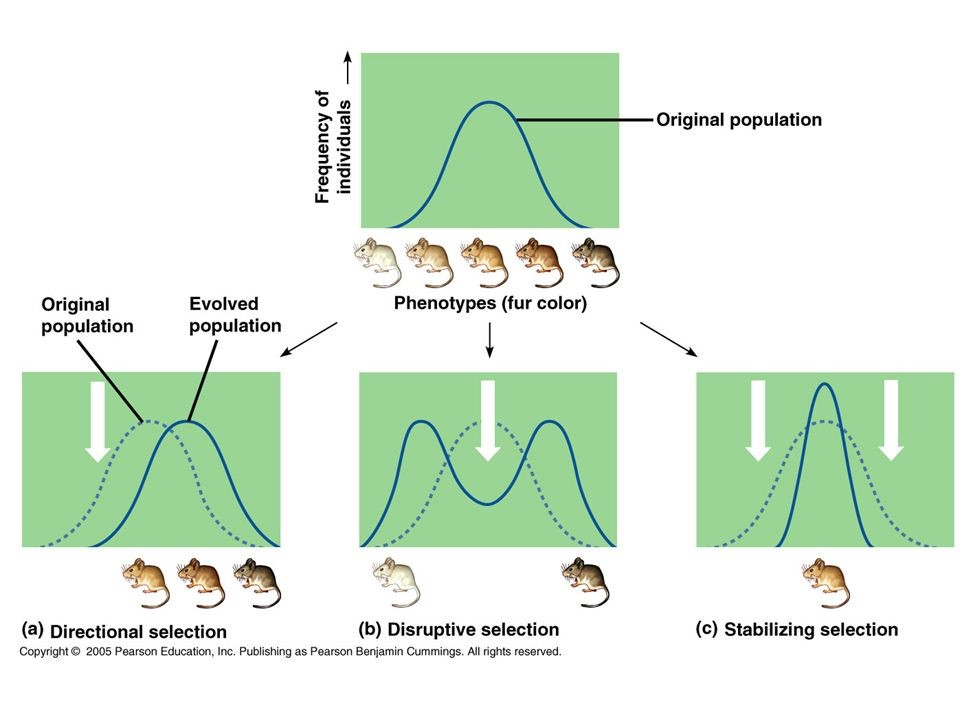
\includegraphics[width=10cm, center]{natural-selection.jpg}
\caption{天擇的方向} \vskip 10 pt
\label{fig:natural-selection}
\end{figure}
\noindent
\begin{enumerate}
\item \textbf{你覺得哪一種天擇最常發生?} \\
\item \textbf{為什麼當談到微演化時,我們都說是「基因」頻率,卻又說天擇偏好的是「表現型」?} \\
\item \textbf{要怎麼觀察一個族群的演化?} \\
\end{enumerate}


\section{哈溫法則}
在理想族群中經過多個世代交替後,基因型頻率會保持恆定且穩定的平衡狀態。 \\

理想族群:
\begin{enumerate}
\item 沒有\underline{\hspace{4em}}發生。
\item 沒有個體的\underline{\hspace{4em}}或\underline{\hspace{4em}}。
\item 族群\underline{\hspace{4em}}。
\item 族群內隨機交配,每一種基因有同等機會傳到後代。
\item 在族群延續過程中,對偶基因(基因組)均相同。
\end{enumerate}

\noindent
例:顯性等位基因記為A而隱性等位基因記為a,它們的頻率分別記為p和q。(記為$f(A) = p, f(a) = q$)。則得知$p + q = 1$ \\
如果群體處於平衡狀態,那我們可以得到:\\
群體中純合子AA的頻率$f(AA) = p^2$ \\
群體中純合子aa的頻率$f(aa) = q^2$ \\
群體中雜合子Aa的頻率$f(Aa) = 2pq$ \\

\begin{figure}[H]
\graphicspath{{biology/}}
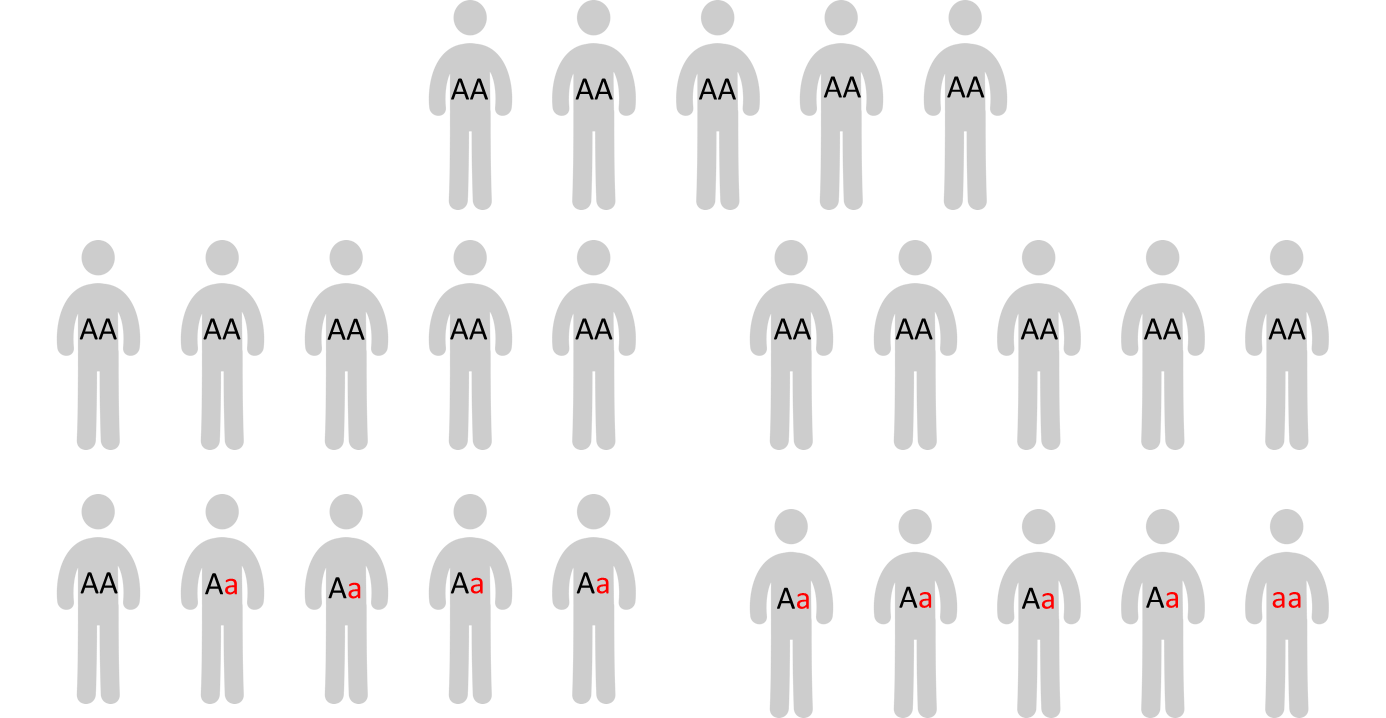
\includegraphics[width=\textwidth, center]{genetic.png}
\caption{等位基因的遺傳} \vskip 10 pt
\label{fig:genetic}
\end{figure}

依性狀由A跟a控制,25人中,有1個隱性性狀者(aa),則: \\
$$q^2 = \frac{1}{25} = 0.04 \rightarrow q=0.2, p=0.8 $$ \\
則推知:
\begin{table}[H]
\centering
\begin{tabular}{|c|c|c|}
\hline
基因型 & 比例          & 人數               \\ \hline
AA  & $(0.8)^2$      & $0.64 \times 25 = 16$ 人 \\ \hline
aa  & $(0.2)^2$      & $0.04 \times 25 = 1$  人 \\ \hline
Aa  & $2(0.8)(0.2)$ & $0.32 \times 25 = 8$  人  \\\hline
\end{tabular}
\end{table}

\noindent
\fbox{小練習}

在一族群中,某基因座有兩種等位基因,16人的基因型為AA,60人為Aa,24人為aa,請用哈溫法則檢視此基因是否在演化。

\section{講師介紹}
\begin{itemize}
\item 姓名:高語儂
\item 性別:女
\item 特色:自己的想法很多、熟捻多國語言、曾任班長但在連任選舉中慘敗、其兄目前就讀香港大學財金系大一,並以學測滿級分(是75喔不是60)同時錄取台大電機系,但講師本人並無特別成就、其父曾經指導國際數學奧林匹亞之選手(編按:詳請請洽講師)...
\item 名言:雪豹好可愛!!!、我哥超認真準備科學班結果沒上,然後我根本沒準備就上了(編按:科學班有單一性別保障6位)。
\end{itemize}

\begin{figure}[H]
\graphicspath{{biology/}}
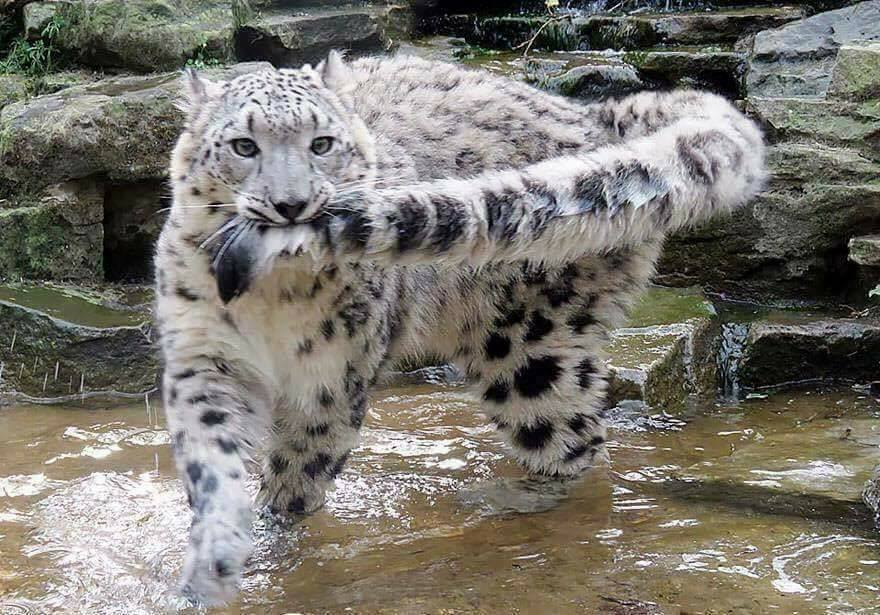
\includegraphics[width=12cm, center]{snowLeopard.jpg}
\caption{講師的最愛:雪豹咬尾巴} \vskip 10 pt
\label{fig:snowLeopard}
\end{figure}
\chapter{觀念分子生物學}
\chapterauthor{李訓至}

\section{附錄}
\subsection{遺傳密碼表}

\begin{figure}[H]
\centering
\graphicspath{{biology/}}
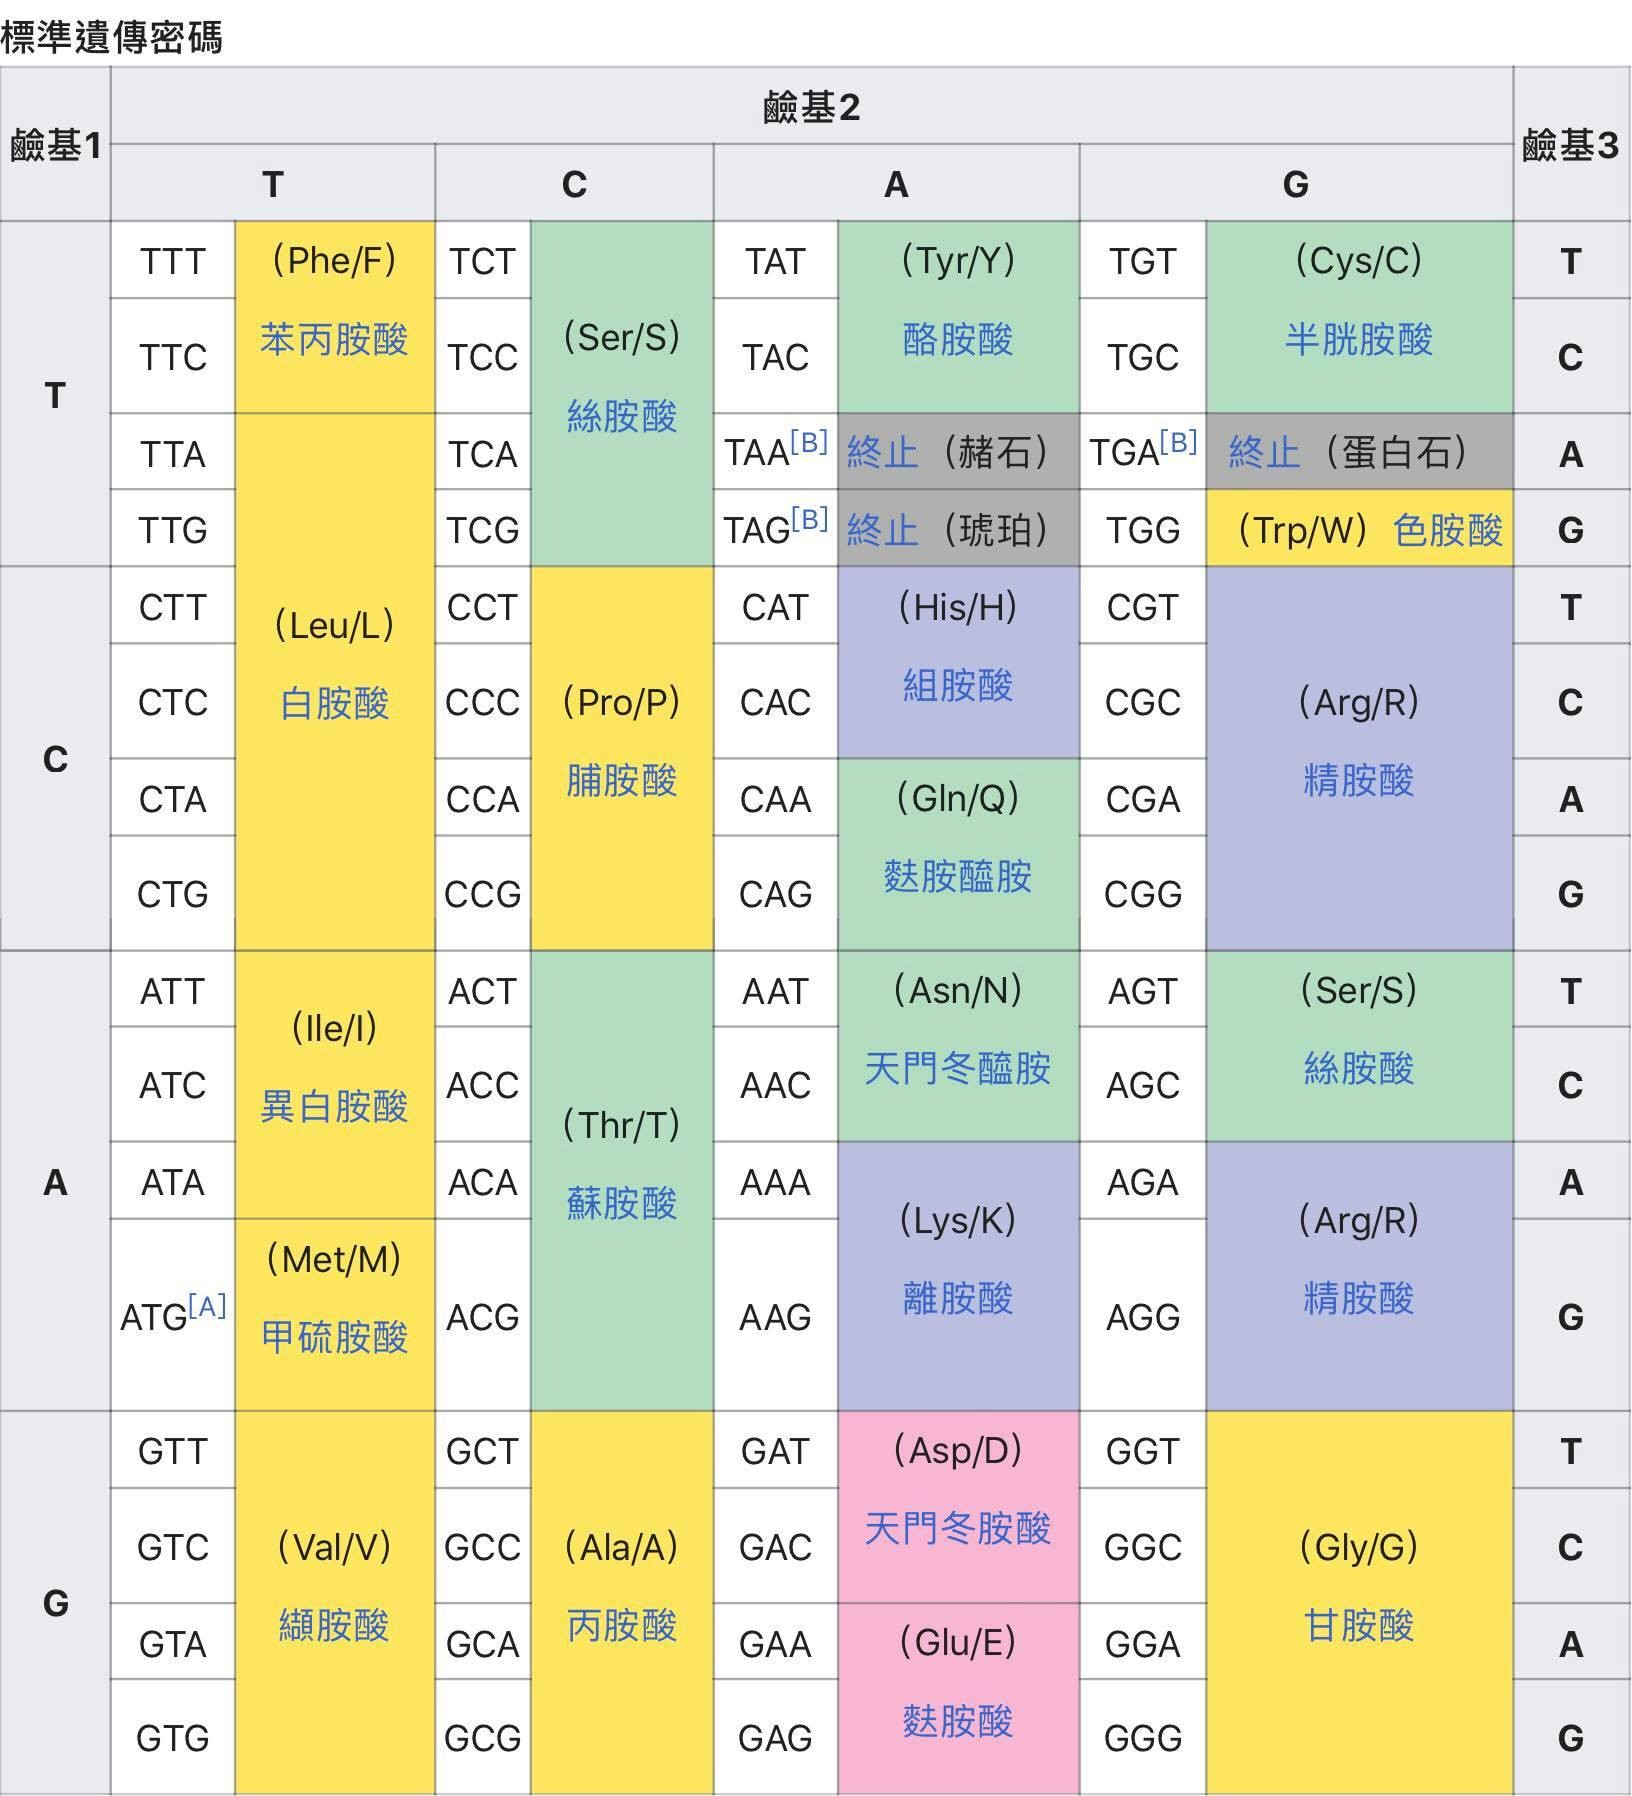
\includegraphics[width=7.5cm, center]{protein.jpg}
\caption{遺傳密碼表(from Wikipedia)} \vskip 10 pt
\label{fig:code}
\end{figure}

\subsection{分子生物學的中心教條}

\begin{figure}[H]
\centering
\graphicspath{{biology/}}
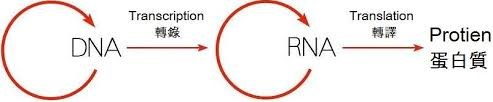
\includegraphics[width=7.5cm, center]{DNA.jpg}
\caption{分生的中心教條} \vskip 10 pt
\label{fig:DNA}
\end{figure}

\section{講師介紹}
\begin{itemize}
\item 姓名:李訓至
\item 性別:男
\item 特色:Minecraft愛好者、曾因為在英文課時沒有將英文課本拿出而多次被英文老師念、繪畫功力一流、會阻止大家刷存在
\item 名言:XXX不要刷存在
\end{itemize}
\part{化學}
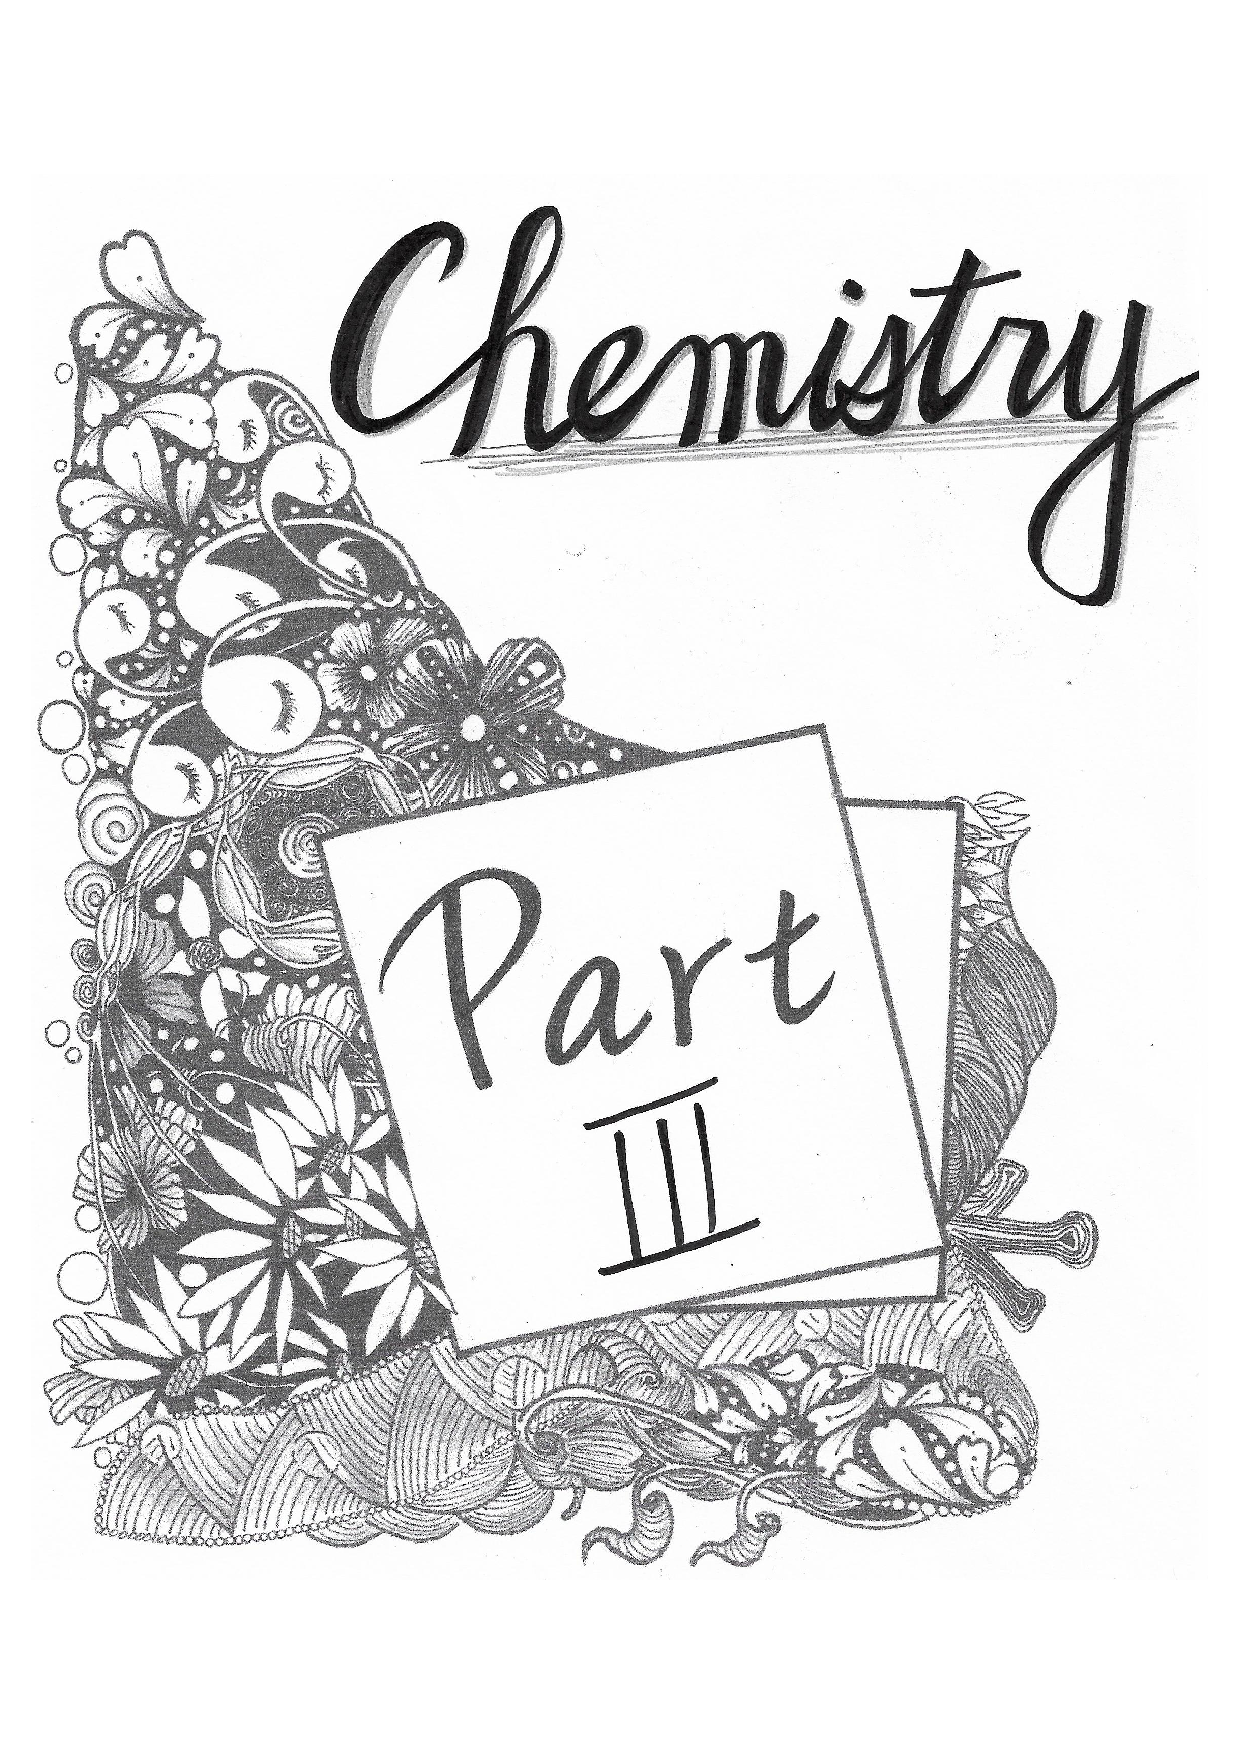
\includepdf[scale=0.9]{partImage/part3.pdf}
\chapter{熱化學與化合物的形成}
\chapterauthor{張竣程}

\section{分子內能及焓}
\begin{gather*}
\boxed{\rm \Updelta E \equiv Q+W} \\
\rm \Updelta E = E_f - E_i = \mbox{內能變化} \\
\rm Q : \mbox{熱} \\
\rm W : \mbox{功}
\end{gather*}
其中(此式推導請看\ref{w=pv}):
\begin{gather}
\boxed{\rm W=- P \Updelta V}
\end{gather}
故:
\begin{enumerate}
\item $\rm \Updelta V = 0$時:
\begin{equation}
\rm \Updelta E = Q
\end{equation}
\item $\rm P$ 為一定值時:
\begin{gather}
\rm \Updelta E = \rm Q_p -P \Updelta V  \\ 
\rm \Updelta E = \rm Q_p - (PV_1 - PV_2) = E_2 - E_1 \\  
\rm \Rightarrow Q_p = \rm (E_2+PV_2)-(E_1+PV_1) \label{Q_p}
\end{gather}
\end{enumerate} 
綜合以上,我們可以定義一個新的物理量:
\theoremstyle{definition}
\begin{gather*}
\rm H\mbox{(焓)} \equiv E + PV \\
\end{gather*}
且由於\eqref{Q_p}可知:
\begin{gather*}
\rm \Updelta H = H_2 - H_1 \\
\rm \Updelta H = (E_2+PV_2)-(E_1+PV_1) \\
\rm \Rightarrow \Updelta H = Q_p
\end{gather*}
\newpage
\section{吸熱與放熱}
\begin{figure}[H]
\centering
\begin{minipage}{0.5\textwidth}
\graphicspath{{chemistry/}}
\includegraphics[width=\linewidth, center]{放熱.jpg}
\caption{放熱反應, 其$\rm \Updelta H<0 \rightarrow$放熱}
\label{fig:exothermal}
\end{minipage}%
\begin{minipage}{0.5\textwidth}
\centering
\graphicspath{{chemistry/}}
\includegraphics[width=\linewidth, center]{吸熱.jpg}
\caption{吸熱反應, 其$\rm \Updelta H>0 \rightarrow$吸熱}
\label{fig:endthermal}
\end{minipage}
\end{figure}

\section{熱反應式及標準狀態}
\subsection{熱反應式表示式}
	\begin{enumerate}
	\item $\rm \mbox{反應物}+\Updelta H \rightarrow \mbox{生成物}$
	\item $\rm \mbox{反應物}\rightarrow \mbox{生成物} \, \, \Updelta \rm H = x \rm \, kcal$(此種表示較常使用)
	\end{enumerate}
\subsection{標準狀態(standard state)}
標準狀態為在一大氣壓力下,某一特定溫度的狀態。國際標準指在1atm 和298K (25°C)的狀態。
\section{生成熱($\rm\Updelta H^{\circ}_f$)}
\begin{enumerate}
\item 元素在標準狀態下以最穩定結構存在時,定其生成熱為0 \\
EX: 石墨(C)、白磷(P)、斜方硫(S)
\item 化合物之反應熱訂為由元素的最穩定態合成化合物的焓變化量(目標化合物之係數必為一) \\
EX: $\rm Pb_{(s)}+\frac{1}{8}S_8+2O_2 \rightarrow PbSO_{4(s)}\quad \Updelta H^{\circ}_f=-219.87 \, kcal$

\end{enumerate}
\section{燃燒熱($\rm\Updelta H^{\circ}_c$)}
$\rm \Updelta H^{\circ}_c$ 為1mol反應物和$\rm O_2$於25℃ 完全反應的焓變化量(若生成物生成時處於高溫狀態,則待其溫度降至25℃時再總計焓變化量) \\
所有放熱反應的$\rm \Updelta H^{\circ}_c$皆為負數:\\
$$\rm Hg_{(l)} + \frac{1}{2} O_2 \rightarrow HgO_{(s)} \quad \Updelta H^{\circ}_c=-21.71 \quad kcal$$

\section{赫斯定律(Hess's Law)}
\begin{enumerate}
\item 正反應與逆反應之$\Updelta \rm H$互為相反數
\item 因為能量守恆的緣故,各化學反應式的焓變化量可以加成
\item \textbf{赫斯定律(Hess's Law):} \\
若一反應為:
\begin{equation}
\rm X + \rm Y \rightarrow \rm Z \label{X+Y}
\end{equation}
且已知有兩反應為:
\begin{equation}
\rm A + B \rightarrow  X \quad \Updelta  H=\Updelta  H_1 \label{A+B}
\end{equation}
\begin{equation}
\rm C + D \rightarrow  Y \quad \Updelta  H=\Updelta  H_2 \label{C+D}
\end{equation}
將\eqref{A+B}與\eqref{C+D}相加可以得到:
\begin{equation}
\rm A+B+C+D \rightarrow  X+Y \quad \Updelta  H = \Updelta H_1 + \Updelta  H_2
\end{equation}
又因為\eqref{X+Y},我們最後可以得到:
\begin{equation}
\rm A+B+C+D \rightarrow  Z \quad \Updelta  H = \Updelta H_1 + \Updelta  H_2 
\end{equation}

\end{enumerate}
\section{其餘特殊的熱能}
\subsection{游離能}
從 1 mol 氣態原子或離子移去最易游離電子的反應熱稱為第一游離能($\rm \Updelta H^{\circ}_1$),移去兩個則稱為第二游離能($\rm \Updelta H^{\circ}_2$)
$$ \rm Na_{(g)} \rightarrow Na^{+}_{(g)}+e^- \quad \Updelta H^{\circ}_1 = 120.04 \, kcal $$
\subsection{電子親和力}
1 mol 氣態原子與 1 mol 電子結合的反應熱
$$ \rm Cl_{(g)} + e^- \rightarrow Cl^-_{(g)} \quad \Updelta \rm H^{\circ}=-87.90 \, kcal$$
\subsection{格子能}氣態離子結合並結晶成離子固體的能量
$$\rm Al^{3+}_{(g)}+3Cl^-_{(g)}\rightarrow AlCl_3 \quad \Updelta H=-1302.6 \, kcal $$
\subsection{水合能}1 mol 氣態離子與水結合成水合物的能量
$$\rm Al^{3+}_{(g)}\xlongrightarrow{H_2O} Al^{3+}_{(aq)} \quad \Updelta H=1438.0 \, kcal$$

\section{一反應式的能量圖}
\begin{figure}[H]
\graphicspath{{chemistry/}}
\includegraphics[width=6cm, center]{energy.jpg}
\caption{一反應式的能量圖} \vskip 10 pt
\label{fig:energy}
\end{figure}
\noindent
其中:\\
$\rm \Updelta H_1:\mbox{昇華能}$ \\ 
$\rm \Updelta H_2:\mbox{游離能}$ \\
$\rm \Updelta H_3:\frac{1}{2} \mbox{鍵解離能}$ \\ 
$\rm \Updelta H_4:\mbox{電子親和力}$ \\ 
$\rm \Updelta H_5:\mbox{格子能}$ \\ 
$\rm \Updelta H_f:\Updelta H_1+\Updelta H_2+\Updelta H_3+\Updelta H_4+\Updelta H_5$


\section{以一反應式的完整步驟計算標準反應熱 (例子)}
試求:$\rm Na_{(s)}+\frac{1}{2}Cl_{2(g)}\rightarrow NaCl_{(s)}$的標準反應熱? \\
解法:
\begin{align}
\rm Na_{(g)} \rightarrow Na^+_{(g)}+e^- \quad \Updelta H^{\circ}&=120.04 \, \rm kcal \mbox{(游離能)} \label{IE} \\
\rm Cl_{(g)}+e^- \rightarrow Cl^-_{(g)} \quad \Updelta H^{\circ}&=-87.9 \, \rm kcal \mbox{(電子親和力)} \label{E_ea} \\
\rm Na^+_{(g)}+Cl_{(g)}\rightarrow NaCl_{(s)} \quad \Updelta H^{\circ}&=-185.4 \, \rm kcal \mbox{(格子能)} \label{LE}
\end{align}
由(\ref{IE}) (\ref{E_ea}) (\ref{LE}) 相加可得:
\begin{align}
\rm Na_{(g)} + Cl_{(g)} \rightarrow NaCl_{(s)} \quad \Updelta H^{\circ}&=-153.3 \, \rm kcal \label{com}
\end{align}
接著:
\begin{align}
\rm Na_{(s)} \rightarrow Na_{(g)} \quad \Updelta H^{\circ}&=25.98 \, \rm kcal \mbox{(昇華能)} \label{SHE} \\
\rm \frac{1}{2} Cl_{2(g)} \rightarrow Cl_{(g)} \quad \Updelta H^{\circ}&=29.082 \, \rm kcal (\frac{1}{2} \mbox{鍵解離能}) \label{BE}
\end{align}
將(\ref{com})(\ref{SHE})(\ref{BE})相加可得
\begin{align}
\rm Na_{(s)}+\frac{1}{2}Cl_{2(g)}\rightarrow NaCl_{(s)} \quad \Updelta H^{\circ}&=-98.2 \, \rm kcal
\end{align}
\section{附錄}
\subsection{符號一覽表:}
	\begin{itemize}
	\item $\Delta$:變化量(末減初)
	\item $\rm \Updelta H$:焓變化量
	\item $\rm\Updelta H^{\circ}_f$:生成熱
	\item $\rm\Updelta H^{\circ}_c$:燃燒熱
	\item $\rm \Updelta H^{\circ}$:標準狀態時的焓變化量
	\item (s):固態, (l):液態, (g):氣態, (aq):水溶液, 水合物
	\item $\rm e^-$:電子
	\item $\rm Pb$:鉛, $\rm S$:硫, $\rm O$:氧, $\rm PbSO_4$:硫酸鉛, $\rm Hg$:汞, $\rm HgO$:氧化汞, $\rm Al$:鋁
	\end{itemize}
\subsection{$\rm W=-P \Updelta V$ 的推導:} \label{w=pv}
\noindent
\textbf{由功的定義:} \\
$$\rm W = F \cdot x $$ 
\textbf{我們可以令:} 
\begin{gather*}
\rm W=F \cdot \Updelta x=PA \Updelta x \\
\rm \Updelta V = -A \cdot \Updelta x
\end{gather*}
\textbf{因此有:} \\ 
\begin{gather*}
\boxed{\rm W =-P\Updelta V} \\
\mbox{(在此狀況中,體積為縮減的,固帶負號)}
\end{gather*}
\subsection{離子鍵與共價鍵的能量關係:}
	\subsubsection{離子鍵為兩原子對電子的吸引力相差的非常大時所產生的,反之,共價鍵為兩原子對電子的吸引力差距不大時所形成的。}
	\subsubsection{若一化合物為離子化合物:}
	$$ \rm \Updelta H_f < 0 $$ \\
	原因:因為此化合物生成時為放熱反應,故在能量上是有利於反應進行
	\subsubsection{若一化合物為共價化合物:}
	$$ \rm \Updelta H_f > 0 $$ \\
	原因: 因為此化合物生成時為吸熱反應,故在能量上是不利於反應進行

	
\newpage
\subsection{常用標準生成熱表:}
\begin{longtable}{|c|c|c|}
\hline
\textbf{化學物質} & \textbf{分子式} & $\rm\Updelta H^{\circ}_f(kJ/mol)$ \\ \hline
氨(aq)         & $\rm NH_3$          & -80.8                   \\ \hline
氨(g)          & $\rm NH_3$          & -46.1                   \\ \hline
碳(石墨)         & C            & 0                       \\ \hline
碳(金剛石)        & C            & 1.9                     \\ \hline
碳(g)          & C            & 718.9                   \\ \hline
一氧化碳          & CO           & -110.6                  \\ \hline
二氧化碳(g)       & $\rm CO_2$          & -393.8                  \\ \hline
二氧化碳(aq)      & $\rm CO_2$          & -413.2                  \\ \hline
碳酸鈉           & $\rm Na_2CO_3$       & -1131                   \\ \hline
氯化鈉(aq)       & NaCl         & -407                    \\ \hline
氯化鈉(s)        & NaCl         & -411.12                 \\ \hline
氯化鈉(l)        & NaCl         & -385.92                 \\ \hline
水(g)          & $\rm H_2O$          & -242                    \\ \hline
氫氧化鈉(aq)      & NaOH         & -469.6                  \\ \hline
氫氧化鈉(s)       & NaOH         & -426.7                  \\ \hline
硝酸鈉(aq)       & $\rm NaNO_3$        & -446.2                  \\ \hline
硝酸鈉(s)        & $\rm NaNO_3$        & -424.8                  \\ \hline
二氧化硫          & $\rm SO_2$          & -297                    \\ \hline
二硫化碳(l)       & $\rm CS_2$          & -89.41                  \\ \hline
二硫化碳(g)       & $\rm CS_2$          & -117.1                  \\ \hline
硫酸            & $\rm H_2SO_4$        & -814                    \\ \hline
二氧化矽          & $\rm SiO_2$         & -911                    \\ \hline
二氧化氮          & $\rm NO_2$          & 33                      \\ \hline
一氧化氮          & NO           & 90                      \\ \hline
水(l)          & $\rm H_2O$          & -286                    \\ \hline
氯化鈉(g)        & NaCl         & -181.42                 \\ \hline
氫             & $\rm H_2$           & 0                       \\ \hline
氟             & $\rm F_2$           & 0                       \\ \hline
氯             & $\rm Cl_2$          & 0                       \\ \hline
溴(l)          & $\rm Br_2$          & 0                       \\ \hline
溴(g)          & $\rm Br_2$          & 31                      \\ \hline
碘(s)          & $\rm I_2$           & 0                       \\ \hline
碘(g)          & $\rm I_2$           & 62                      \\ \hline
\end{longtable}


\section{講師介紹}
\begin{itemize}
\item 姓名:張竣程
\item 性別:男
\item 特色:上課時通常不是在睡覺就是在看漫畫(編按:但還是超電)、在國中時期吃遍各種顏色的粉筆(編按:可以詢問講師他覺得哪一種顏色的粉筆比較好吃喔),甚至是蝴蝶、聽說在科班入學考試中拿到第二名的成績、熟捻所有周星馳電影,能將台詞及角色倒背如流。
\item 名言:考試靠賽,輕鬆自在、我以後要當尼特族!!!
\end{itemize}
\chapter{手搖手工皂}

\section{實驗原理}
動物脂肪和植物油主要成份是由長鏈脂肪酸(fatty acids)和甘油所反應而成的酯類。這些三酸甘油酯(triglyceride or triacylglycerol)經過水解反應會產生甘油和脂肪酸鹽。因為脂肪酸鈉鹽是離子化合物,如果濃度很低時,它是溶在水中的,但是如果高濃度的脂肪酸鈉鹽,它會聚集在一起而凝集形成了肥皂。基本上,酯類的水解反應被稱為皂化(saponification),其反應式如圖所示,其中R為長鏈的飽和或不飽和的烴基。

\begin{figure}[H]
\centering
\graphicspath{{chemistry/}}
\includegraphics[width=\textwidth, center]{fatty.png}
\caption{皂化反應} \vskip 10 pt
\label{fig:soap}
\end{figure}

\section{實驗器材及藥品}
\begin{table}[H]
\centering
\begin{tabular}{|c|c|}
\hline
\textbf{實驗器材} & \textbf{實驗藥品} \\ \hline
\begin{tabular}[c]{@{}c@{}}空寶特瓶罐X1\\   磅秤 數個\\   秤量紙 數張\\   燒杯X2\\   玻棒X1\\   空紙杯X1\end{tabular} & \begin{tabular}[c]{@{}c@{}}NaOH 7g\\   $\rm KOH$ 10g\\   $\rm H_{2}O$ 46.3g\\   棕櫚油 50g\\   紅色染料\\   黃色染料\\   玫瑰水\end{tabular} \\ \hline
\end{tabular}
\end{table}

\section{實驗步驟}
\begin{enumerate}
\item 秤出7g NaOH 和10g KOH
\item 用燒杯裝 43.6g $\rm H_{2}O$,並將秤好的NaOH和KOH倒入燒杯並溶解
\item 在寶特瓶內裝入50g棕櫚油並加入步驟2配好的溶液
\item 鎖緊瓶蓋,搖晃瓶身直到混和液變濃稠
\item 之後可加入玫瑰水和染料並到入空紙杯,等待一個禮拜即可
\end{enumerate}
\part{數學}
\includepdf[scale=0.9]{partImage/part4.pdf}
\chapter{我的改變,你看的見!\\基礎初等微積分}
\chapterauthor{吳冠廷}

\section{函數的極限}
只要$x$越來越靠近,$f(x)$跟極限的距離能比任何正數都還小 \\ \\
定義:\\ \\ 
表示方法:\\ \\
筆記/計算:\\
\newpage
\section{微分}
將兩個極小的數相除,形成斜率。 \\ \\
定義:\\ \\ 
表示方法:\\ \\
筆記/計算:\\
\newpage
\section{積分}
將很多極小的長條相加,形成面積 \\ \\
定義:\\ \\ 
表示方法:\\ \\
筆記/計算:\\
\newpage
\section{附錄}
\subsection{補充資料}
這邊有點難度,不過如果你是天資聰穎(桃園市科學奧林匹亞有得獎就可以了)的國中生,可以去研究一下 \\
\begin{enumerate}
\item \textbf{極限:} \\
公式、羅畢達法則、p級數的次方數與收斂發散關西、等比數列發散收斂條件、交錯級數判別法、各種審斂法
\item \textbf{微分:} \\
泰勒展開式、偏微分、隱含數微分、微分方程、柯西均值定理
\item \textbf{積分:}\\
分布積分法、變數變換法、三角積分法、積球的表面積和體積、積轉動慣量、瑕積分
\end{enumerate}
\subsection{發展學科}
有興趣可以研究、但許多都很難,所以有興趣的話可以認識一下,等數學好再回來(?) \\
\begin{enumerate}
\item \textbf{物理:} \\
力學、電磁學、熱力學、統計力學、相對論、量子力學……(簡單來說就是所有的物理領域)\url{http://bit.ly/2Ujms7f}
\item \textbf{數學:} \\
高等微積分、統計、變分法……
\item \textbf{社會科學:} \\
\url{http://bit.ly/2DcwSjI}
\item \textbf{化學:} \\
\url{http://t.cn/EXL3aB7}, \url{http://bit.ly/2UcTxly}
\item \textbf{生物:} \\
洛特卡-沃爾泰拉方程:\url{http://t.cn/EX2vYfi}\\
計算生物學:\url{http://t.cn/EX2ZDh}, \url{http://bit.ly/2Ug9aIH}
\item \textbf{工科(電機、電子、機械、土木、化工、材料…):} \\
工程數學:\url{http://t.cn/EXLm6Cc}, \url{http://t.cn/EXLu4oz}
\item \textbf{社會科學:} \\
\url{http://t.cn/EKdmEYI}
\end{enumerate}
\subsection{推薦YouTube頻道}
\begin{enumerate}
\item \textbf{3b1b:} \\
有關於微積分的全系列影片,以較視覺化的方法幫助你理解,其他的影片也都很不錯,值得一看~~
\item \textbf{中華科技大學開放式課程──微積分系列:} \\
很清楚且淺顯易懂,適合初學者
\item \textbf{blackpenredpen:} \\
有許多較難的微積分題目及講解,但為英文影片,需有英文基礎
\item \textbf{清華大學開放式課程──高淑蓉教授微積分:} \\
因為是正規課程,所以較嚴謹且有條理,缺點是影片長度長,無法快速上手 \\ \\
\end{enumerate}
\begin{center}
\textbf{\large 有電子書的需求請跟講師說,我可以分享給你~~~}
\end{center}

\section{講師介紹}
\begin{itemize}
\item 姓名:吳冠廷
\item 性別:男
\item 特色:桌面十分雜亂,寫出的字也非常瀟灑(編按:但國中時期的字非常漂亮)、具有領導力、笑聲十分經典、會在黑特武陵留言裝弱,比熊熊還誇張。
\item 名言:哈哈哈哈哈哈!!!、沒差拉那個不是重點!
\end{itemize}
\chapter{碎形\\跨越維度的奇幻之旅}
\chapterauthor{陸柏丞}

\section{先備知識}
\subsection{相似}
\noindent
\subsubsection{定義:}
\vspace{2.5em}
\subsubsection{相似圖形邊長,面積,和體積的關係:}
\vspace{2.5em}
\textbf{假設圖形$F$和圖形$G$相似,$F$和$G$的相似比為$1$比$k$,那麼$F$和$G$的面積比為$1$比$k^2$;體積比為1比$k^3$。}

\subsection{指數函數}
\noindent
\subsubsection{定義:}
\subsubsection{例如:}
\subsection{無限}
\noindent
定義:
\newpage
\section{自我相似}
\subsection{製作考區曲線 (Koch Curve)}
\vspace{7.5cm}
\begin{enumerate}
\item 每一張圖的圖形總長度有規律嗎?規律是甚麼?可否解釋這個規律的來源?
\item 圖形中,那些部分有相似呢?
\end{enumerate}
\subsection{製作史賓斯基地毯 (Sierpinski Carpet)}
\vfill
\begin{enumerate}
\item 每一張圖的圖形剩餘面積有規律嗎?規律是甚麼?
\item 圖形中,那些部分有相似呢?
\end{enumerate}
\section{碎形(fractal)}
數學家:曼德布洛特 (Benoit B. Mandelbrot, 1924-2010)
定義;「一個粗糙或零碎的幾何形狀,可以分成數個部分,且每一部分都(至少近似地)是整體縮小後的形狀」考區曲線及史賓斯基地毯極為碎形的典型例子。

問:真正的碎形存在嗎?\\
其實,考區曲線和史賓斯基地毯確實存在,只是我們無法看見,活動一和活動二圖案只是重複幾何操作有限次就停止的仿冒圖。

雖然完美的碎形在生活中不存在,生活中處處皆充滿自我相似的物品,例如:花椰菜、血管分支、積雨雲、閃電、布朗運動等。而碎形理論可以完整的解釋生活中這些自我相似的事物。
\section{碎形的維度}
\subsection{問題與討論}
\begin{enumerate}
\item 考區曲線有多長呢?
\item 考區曲線包圍的面積有多大呢?
\item 史賓斯坦地毯周長有多長呢?
\item 史賓斯坦地毯面積多大呢?
\end{enumerate}
看來考區曲線和史賓斯基地毯的真正面貌與大家的印象截然不同。

\begin{itemize}
\item 考區曲線:周長無限大的鋸齒狀圖形,且貼在平面特定區域內。
\item 史賓斯坦地毯:周長無限大,面積卻是零的國王的地毯。
\end{itemize}

模糊的文字很難說明碎形真正的樣貌;然而,聰明的數學家豪斯多夫巧妙的使用維度來定義碎形。
\subsection{計算維度}
\subsubsection{維度$k$和拼排個數的法則}
把$n \cdot k$個縮小$n$倍的相似圖形加起來等於1。為了瞭解上述定義,我們來討論縮放倍率與質量的關係。
\begin{enumerate}
\item 正方形 \\

\item 正方體 \\

\item 考區曲線 \\

\item 史賓斯基地毯 \\

\end{enumerate}

\section{講師介紹}
\begin{itemize}
\item 姓名:陸柏丞
\item 性別:男(不過沒辦法定論是不是人類)
\item 特色:啊$\sim\sim\sim\sim$、對朋友的定義很奇怪,可能對他來說還沒記住名字的是"朋友"、開冷氣一定要投票、對英文雜誌情有獨鍾、喜歡跟別人在浴室聊天、會撿肥皂抹你的臉、曾提出"陸三點":要讀書、要認真、要投票
\item 名言:我今天早上只跑了五圈操場,然後去跟學長打球,我好懶惰喔。
\end{itemize}

\chapter{三角函數\\簡單定義及演算}
\chapterauthor{黃裕盛}

\setcounter{section}{-1}
\section{引導}
我知道你們看到標題會覺得很@@,三角函數怎麼可能會簡單? \\
希望在這堂課之後,可以克服對他的恐懼 :) (希望是不要加深啦)

\section{觀念}
\subsection{相似}
\subsubsection{定義}
兩個三角形的對應角相等,而對應邊成比例。

\subsubsection{判別種類}
\begin{enumerate}
\item AA相似
\item SAS相似
\item SSS相似
\end{enumerate}

\subsection{畢氏定理}
\subsubsection{定義}
當一個三角形為直角三角形時,其兩股平方和等於斜邊長。 \\
怎麼說呢?如下圖: \\

\definecolor{wrwrwr}{rgb}{0.3803921568627451,0.3803921568627451,0.3803921568627451}
\definecolor{rvwvcq}{rgb}{0.08235294117647059,0.396078431372549,0.7529411764705882}
\newpage
\begin{figure}[H]
\centering
\begin{tikzpicture}[line cap=round,line join=round,>=triangle 45,x=1.5cm,y=1.5cm]
%\clip(-2.505849312497348,-1.2756636626591513) rectangle (6.856860587833347,3.6499707160434913);
\fill[line width=2pt,color=rvwvcq,fill=rvwvcq,fill opacity=0.10000000149011612] (0,3) -- (3,0) -- (0,0) -- cycle;
\draw[line width=2pt,fill=black,fill opacity=0.10000000149011612] (0.1698999741866448,0) -- (0.16989997418664482,0.1698999741866448) -- (0,0.1698999741866448) -- (0,0) -- cycle; 
\draw [line width=2pt,color=rvwvcq] (0,3)-- (3,0);
\draw [line width=2pt,color=rvwvcq] (3,0)-- (0,0);
\draw [line width=2pt,color=rvwvcq] (0,0)-- (0,3);
\begin{scriptsize}
\draw [fill=rvwvcq] (0,3) circle (2.5pt);
\draw[color=rvwvcq] (0.06509155833768435,3.1734256013559996) node {$A$};
\draw [fill=rvwvcq] (3,0) circle (2.5pt);
\draw[color=rvwvcq] (3.060517993516196,0.16999000458609542) node {$B$};
\draw [fill=wrwrwr] (0,0) circle (2.5pt);
\draw[color=wrwrwr] (0.06509155833768435,0.16999000458609542) node {$C$};
\draw[color=rvwvcq] (1.4346581904647575,1.507519990347626) node {$c$};
\draw[color=rvwvcq] (1.5307681295613944,0.2260541357258003) node {$a$};
\draw[color=rvwvcq] (0.15319233584293468,1.5956207678528767) node {$b$};
\draw[color=black] (0.5376320922294816,0.36220988277936933) node {$\alpha = 90\textrm{\degre}$};
\end{scriptsize}
\end{tikzpicture}
\caption{直角三角形} \vskip 10 pt
\label{fig:right-tri}
\end{figure}

\noindent
在$\rm \bigtriangleup ABC$內$a^2 + b^2 = c^2$,這就是畢氏定理喔。\\
當今證明畢氏定理的方法有太多種了,我還是講解最簡單的那一種吧。 \\
\begin{proof}
\end{proof}
\newpage

\section{定義}
\subsection{前提}
兩直角三角形若其中一銳角相等,則兩邊比值相同,而無關大小及位置(By AA相
似),如下圖: \\
$\because \angle C = \angle D = 90^{\circ}; \angle B = \angle E \therefore \overline{AC} : \overline{FD} = \overline{CB} : \overline{DE}$
\begin{figure}[H]
\centering
\begin{tikzpicture}[line cap=round,line join=round,>=triangle 45,x=1cm,y=1cm]
%\clip(-8.386803745862085,-2.0982104574476206) rectangle (11.193489106455077,8.202799041419008);
\fill[line width=2pt,color=rvwvcq,fill=rvwvcq,fill opacity=0.10000000149011612] (-3,3) -- (-1,0) -- (-3,0) -- cycle;
\fill[line width=2pt,color=rvwvcq,fill=rvwvcq,fill opacity=0.10000000149011612] (1,0) -- (5,0) -- (1,6) -- cycle;
\draw[line width=2pt,fill=black,fill opacity=0.10000000149011612] (-2.644687138062653,0) -- (-2.644687138062653,0.3553128619373469) -- (-3,0.3553128619373469) -- (-3,0) -- cycle; 
\draw[line width=2pt,fill=black,fill opacity=0.10000000149011612] (1.355312861937347,0) -- (1.355312861937347,0.3553128619373469) -- (1,0.3553128619373469) -- (1,0) -- cycle; 
\draw [line width=2pt,color=rvwvcq] (-3,3)-- (-1,0);
\draw [line width=2pt,color=rvwvcq] (-1,0)-- (-3,0);
\draw [line width=2pt,color=rvwvcq] (-3,0)-- (-3,3);
\draw [line width=2pt,color=rvwvcq] (1,0)-- (5,0);
\draw [line width=2pt,color=rvwvcq] (5,0)-- (1,6);
\draw [line width=2pt,color=rvwvcq] (1,6)-- (1,0);
\begin{scriptsize}
\draw [fill=rvwvcq] (-3,3) circle (2.5pt);
\draw[color=rvwvcq] (-2.859432795250738,3.3537872529281314) node {$A$};
\draw [fill=rvwvcq] (-1,0) circle (2.5pt);
\draw[color=rvwvcq] (-0.8662293312424045,0.355607252444999) node {$B$};
\draw [fill=rvwvcq] (-3,0) circle (2.5pt);
\draw[color=rvwvcq] (-3.479168326076859,0.33885764350375247) node {$C$};
\draw[color=rvwvcq] (-2.1726988286596316,1.544829487273504) node {$c$};
\draw[color=rvwvcq] (-1.9382043034821808,0.4728545150337249) node {$a$};
\draw[color=rvwvcq] (-2.6751870968970266,1.6955759677447229) node {$b$};
\draw [fill=rvwvcq] (1,0) circle (2.5pt);
\draw[color=rvwvcq] (0.5574874287635483,0.30535842562125937) node {$D$};
\draw [fill=rvwvcq] (5,0) circle (2.5pt);
\draw[color=rvwvcq] (5.130130669723844,0.355607252444999) node {$E$};
\draw [fill=rvwvcq] (1,6) circle (2.5pt);
\draw[color=rvwvcq] (1.1269741327659293,6.351967253411264) node {$F$};
\draw[color=rvwvcq] (3.0531791610092776,-0.0631329710861647) node {$f$};
\draw[color=rvwvcq] (3.2876736861867286,3.3537872529281314) node {$d$};
\draw[color=rvwvcq] (0.7919819539409994,3.2030407724569123) node {$e$};
\draw[color=black] (-2.0387019571296596,0.3221080345625059) node {$\alpha = 90\textrm{\degre}$};
\draw[color=black] (1.8807065351220222,0.3221080345625059) node {$\beta = 90\textrm{\degre}$};
\end{scriptsize}
\end{tikzpicture}
\caption{AA相似} \vskip 10pt
\label{fig:AA-tri}
\end{figure}

\subsection{定義}
\noindent
如下圖:$\overline{AC}$稱為$\angle A$的鄰邊,$\overline{BC}$稱為$\angle A$的對邊,$\overline{AB}$稱為斜邊。

\begin{figure}[H]
\centering
\begin{tikzpicture}[line cap=round,line join=round,>=triangle 45,x=1.5cm,y=1.5cm]
%\clip(-2.505849312497348,-1.2756636626591513) rectangle (6.856860587833347,3.6499707160434913);
\fill[line width=2pt,color=rvwvcq,fill=rvwvcq,fill opacity=0.10000000149011612] (0,3) -- (3,0) -- (0,0) -- cycle;
\draw[line width=2pt,fill=black,fill opacity=0.10000000149011612] (0.1698999741866448,0) -- (0.16989997418664482,0.1698999741866448) -- (0,0.1698999741866448) -- (0,0) -- cycle; 
\draw [line width=2pt,color=rvwvcq] (0,3)-- (3,0);
\draw [line width=2pt,color=rvwvcq] (3,0)-- (0,0);
\draw [line width=2pt,color=rvwvcq] (0,0)-- (0,3);
\begin{scriptsize}
\draw [fill=rvwvcq] (0,3) circle (2.5pt);
\draw[color=rvwvcq] (0.06509155833768435,3.1734256013559996) node {$A$};
\draw [fill=rvwvcq] (3,0) circle (2.5pt);
\draw[color=rvwvcq] (3.060517993516196,0.16999000458609542) node {$B$};
\draw [fill=wrwrwr] (0,0) circle (2.5pt);
\draw[color=wrwrwr] (0.06509155833768435,0.16999000458609542) node {$C$};
\draw[color=rvwvcq] (1.4346581904647575,1.507519990347626) node {$c$};
\draw[color=rvwvcq] (1.5307681295613944,0.2260541357258003) node {$a$};
\draw[color=rvwvcq] (0.15319233584293468,1.5956207678528767) node {$b$};
\draw[color=black] (0.5376320922294816,0.36220988277936933) node {$\alpha = 90\textrm{\degre}$};
\end{scriptsize}
\end{tikzpicture}
\caption{直角三角形} \vskip 10 pt
\label{fig:right-tri}
\end{figure}

\begin{figure}[H]
\centering
\graphicspath{{math/}}
\includegraphics[width=5cm, center]{hex-tri.png}
\caption{神秘的三角函數六邊形} \vskip 10 pt
\label{fig:hex-tri}
\end{figure}

\begin{align*}
\sin A &= \frac{a}{c} \mbox{(稱作正弦值)} \\
\cos A &= \frac{b}{c} \mbox{(稱作餘弦值)} \\
\tan A &= \frac{a}{b} \mbox{(稱作正切值)} \\
\cot A &= \frac{b}{a} \mbox{(稱作餘切值)} \\
\sec A &= \frac{c}{b} \mbox{(稱作正割值)} \\
\csc A &= \frac{c}{a} \mbox{(稱作餘割值)} \\
\end{align*}
※這些名字可以不用記沒關係,然後建議背最上方三個然後倒數變成下面三個。

\subsection{三角函數間的關係}
\subsubsection{平方關係}
\begin{enumerate}
\item ${\sin}^2 + {\cos}^2 = 1$
\item $1 + {\tan}^2 = {\sec}^2$
\end{enumerate}
\subsubsection{相除關係}
\begin{enumerate}
\item $\tan \theta = \frac{\sin \theta}{\cos \theta}$ (尷尬只有這一個)
\end{enumerate}
\subsubsection{倒數關係}
\begin{enumerate}
\item $\sin \theta \cdot \csc \theta = 1$
\item $\cos \theta \cdot \sec \theta = 1$
\item $\tan \theta \cdot \cot \theta = 1$
\end{enumerate}
\subsubsection{餘角關係($90^\circ - \theta$)}
\begin{enumerate}
\item $\sin (90^\circ-\theta) = \cos \theta$;$\cos (90^\circ-\theta) = \sin \theta$
\item $\tan (90^\circ-\theta) = \cot \theta$;$\cot (90^\circ-\theta) = \tan \theta$
\item $\sec (90^\circ-\theta) = \csc \theta$;$\csc (90^\circ-\theta) = \sec \theta$
\end{enumerate}
※證明由圖 \ref{fig:hex-tri}就可以看出喔! \vskip 20 pt

\noindent
\fbox{小練習} \vskip 10 pt
\noindent
$\bigtriangleup ABC$的$\angle A$為銳角,$\angle C=90^\circ$,$\overline{AC}=10$;$\overline{AB}=26$,求$\angle A$的六個三角函數值。
\vspace{5cm}

\noindent
\fbox{小笑話} \vskip 10 pt
\noindent
sin對cos說:買這麼多衣服想玩甚麼?\\
cos說:我想玩cosplay \\


\noindent
\fbox{腦筋急轉彎} \vskip 10 pt
\noindent
$\frac{\sin x}{n} =$ ? \\
\rightline{Ans:6}

\section{講師介紹}
\begin{itemize}
\item 姓名:黃裕盛
\item 性別:男
\item 特色:大電神,非常認真、心算能力頂尖,可在2秒內算出四位數乘四位數、每天固定打一場LOL,但真的就只有打一場、對化學有興趣,跟熊熊借了熊熊很少在看的化學經典教材小銀、喜歡拿橡皮筋彈穿短褲的熊熊,並以此為樂。
\item 名言:這題講義出現過啊,我就直接寫答案了(編按:此為數學段考)。
\end{itemize}
\part{資訊}
\includepdf[scale=0.9]{partImage/part5.pdf}
\chapter{這本講義怎麼做出來的 \\ \LaTeX 教學}
\chapterauthor{李杰穎}
\setcounter{section}{-1}
\section{前言}
Hi各位,我是編這本講義的熊熊,大家有沒有發現這本講義好像不是用Word打出來的,很多地方都跟Word不太一樣。\\
其實這本講義是由\LaTeX 打出來的喔。
\section{蛤,\LaTeX 是甚麼}
{\Kai \LaTeX 是一種基於是一種基於TeX的排版系統,由美國電腦科學家萊斯利·蘭伯特在20世紀80年代初期開發,利用這種格式系統的處理,即使使用者沒有排版和程式設計的知識也可以充分發揮由TeX所提供的強大功能,不必一一親自去設計或校對,能在幾天,甚至幾小時內生成很多具有書籍品質的印刷品。對於生成複雜表格和數學公式,這一點表現得尤為突出。因此它非常適用於生成高印刷品質的科技和數學、物理文件。這個系統同樣適用於生成從簡單的信件到完整書籍的所有其他種類的文件。}\\
\rightline{\textit{from wikipedia}} 

簡單來說,\LaTeX 算是一種寫文件的方法,不過這種方法與一般的文書軟體不同,並不是所見即所得(What You See Is What You Get;WYSIWYG),而是一種類似透過寫程式語言的方法來完成,然後再經過xelatex這種類似程式語言編譯器的``排版引擎"編譯出pdf檔,來生成你們現在看到的文字、數學式、圖片...
\begin{figure}[H]
    \centering
    \graphicspath{{informatics/}}
    \includegraphics[width=5cm, center]{code.png}
    \caption{這章的\LaTeX 原始碼} \vskip 10 pt
    \label{fig:code}
\end{figure}

\section{用\LaTeX 有甚麼好處}
當你使用\LaTeX 來編寫文件、書籍、論文等等...,你不用像Word一樣一直管排版,也不用一直管圖片到底要放在哪裡,大小要多大之類的,你只要專心在你文件的內容,變相提升你的效率。

而且它還可以自動生成目錄,自動生成章節、圖片的編號,相當的強大。

但是它的安裝及文件的版面設定非常不友善,跟Word這種幾乎不用什麼設定的軟體差的非常多,這是\LaTeX 的致命傷之一。

\begin{figure}[H]
    \centering
    \graphicspath{{informatics/}}
    \includegraphics[width=5cm, center]{setting.png}
    \caption{這本講義的前置設定} \vskip 10 pt
    \label{fig:setting}
\end{figure}

\section{\LaTeX 安裝教學}
我這邊有打一份\LaTeX 的安裝教學,對使用\LaTeX 的編寫及使用有興趣的人可以去下面的網址看看。 \\
\url{http://bit.ly/latex-installation}

\section{講師介紹}
\begin{itemize}
\item 姓名:李杰穎
\item 性別:公熊
\item 特色:為班上的存在王,喜愛裝弱和否認自己裝弱,再接著說自己真的很弱。因為戀愛不順常常收好人卡(編按:對熊熊說你是個好人,就會有意料之外的事情喔!),因此埋首在電腦的世界中,是資訊電神喔!他擅長同意別人的說法,和說尷尬笑話,也擅長同意別人說尷尬笑話,所以要說笑話可以去找熊熊喔!
\item 名言:完了、喔不、我是廢物(單邊嘴唇)、你看麻這這這是這樣麻對不對不是麻你看就是是是這樣阿
\end{itemize}
\part{活動}
\includepdf[scale=0.9]{partImage/part6.pdf}
\chapter{世界和平遊戲\\武陵動盪}

\section{遊戲簡介}
本遊戲為回合制遊戲,共三回合,參與小隊將代表不同國家進行遊戲,透過武陵大陸的世界觀,分隊體驗各國狀況,藉由模擬各國互動,準備到時候的緊急狀況。

每個國家會有初始國家人民與資源,包含居民、軍隊、古硬幣、糧食、及科技產品。在遊戲中,你必須盡力爭取資源,已成為進步幅度最大的國家。

國家必須解決遊戲中的危機,以利國家順利運作。你可以透過與其他國家協商獲得危機真相,以避免資源不斷損失。

另外,國家與國家間可互相結盟,亦可以對其他國家發對戰爭。贏家可以掠奪輸家的龐大資源,成為更強盛的國家。

遊戲結束時,各國將依據人民積資源的變化量獲得積分,積分最高者即為世界和平遊戲的贏家!

\section{遊戲規則}
\subsection{國家分配}
參加者將被分為七組,每個小隊會被隨機分配到一個國家,七個國家分別是:

\begin{enumerate}
    \item \textbf{育崇科學合眾國} \\
    前身為術諮班的新派勢力。\textbf{科學班}為此國的重要支柱,強調「重理論輕應用」,講求理論的嚴謹推導,建立許多公理系統。雖然武力不是非常強大,但它們\textbf{國家資產極高},透過極度嚴謹公理約束社會,使用嚴密的策略來與各國外交或對抗。
    \item \textbf{大志青暨原生消費福利聯合王國} \\
    前身為術諮班的舊派勢力。\textbf{術諮班}為此國的重要支柱,強調「重應用輕理論」,研究講求實際應用,努力在原本的基礎上追求革新,任何無實際用途的發明或研究都不被重視,也因此擁有強大的工業實力。另外,此國為原生消費福利自治區的建立國,\textbf{控制武陵大陸的糧食命脈}。
    \item \textbf{建北黑魔法帝國} \\
    此國位於荒涼的台北大莽原,創立者為\underline{\hspace{2em}},他利用神秘的黑魔法及莽原土著的負面情緒,建立了強大的建北黑魔法帝國。因為對武陵興盛的科學發展感到恐懼,此國試圖利用魔力影響武陵大陸人民的作息,以保持自身的地位及安全。而強盛的\textbf{土著勢力}及\textbf{黑科技}讓帝國齊身武力強國。
    \item \textbf{大明道普通共和國}\\
    前身為明道王國。\textbf{普通班}為此國的主要成員,普通表示普遍通用,不跟隨著科學革命的潮流,亦不固守於老舊的術諮主義,它們廣泛涉及多種知識,無論是術諮、科學、美育,各種國家的文化在此處兼容並蓄,可稱為武陵的文化大熔爐,但各知識的能力皆不專精,能力是最平均的一個國家。此國的特色為居民眾多,生產力極高。
    \item \textbf{科教聯邦}\\
    前身為三個自治州:物州、化州、生州。\textbf{設備組}為此聯邦的管理者,他們力量強大,積極保護聯邦內\textbf{豐富的自然資源},如實驗室地形,天然的實驗器材礦產,以及自然生成的資優、創發洞穴,避免珍貴資源被虎視眈眈的強國掠奪。由於他是中立國,所以是最安全的地區,是各國協商及科學推廣隊訓練的最佳選擇。 
    \item \textbf{美育聯合大公國}\\
    \textbf{音樂班}為此國主要成員。此國因為經歷過文藝復興,不崇尚科學,四處充滿著藝術風,比起武力,更注重社會上人與人之間的交際與無私的純樸。另外,優良的家庭背景使此國擁有\textbf{巨額資金}。
    \item \textbf{間諜組織}\\
    此國成員常穿梭於國於國之間搜尋情報,並以\textbf{販賣情報}維生。特殊能力:此國成員在協商階段時,如果申明自己是間諜組織的成員,就有權力詢問任何國家的成員任何問題,被詢問的成員一定要誠實回答每個問題。\\
    遊戲中,小隊將代表自己的國家,進行各項任務與動作。
\end{enumerate}

\subsection{角色分配}
\noindent
各國須選出以下官職:\\
\textbf{皇帝:}國家實質代表,負責統籌意見及下達命令。\\
\textbf{宰相:}管理人民,決定並回報國家生產物資。\\
\textbf{大都督:}管理軍隊,決定戰爭相關事物。當本國國家代表在宣言階段向其他國家開戰時,大都督有否決權。\\
\textbf{官員集團:}其餘玩家都是普通官員,可參與內政討論,負責國際談判。
\subsection{人民與資源說明}
\noindent
\textbf{居民}:國家的主要命脈,可以在每年年初生產物資。\\
\textbf{軍隊}:國家雇用的國際軍隊,負責出征國際戰爭。\\
\textbf{古硬幣}:國家間的流通資金,為國際交易的媒介。\\
\textbf{糧食}:居民及軍隊的維生必需品。\\
\textbf{科技產品}:國家的武力象徵,為發動戰爭的消耗品。\\

下表是各個國家的初始人民及資源:
\begin{table}[H]
\centering
\resizebox{\textwidth}{!}{%
\begin{tabular}{|c|c|c|c|c|c|c|c|}
\hline
 & \begin{tabular}[c]{@{}c@{}}育崇\\ 科學合眾國\end{tabular} & \begin{tabular}[c]{@{}c@{}}大志青暨\\ 原生消費\\ 福利聯合王國\end{tabular} & \begin{tabular}[c]{@{}c@{}}建北\\ 黑魔法帝國\end{tabular} & \begin{tabular}[c]{@{}c@{}}大明道\\ 普通共和國\end{tabular} & \begin{tabular}[c]{@{}c@{}}科教\\ 聯邦\end{tabular} & \begin{tabular}[c]{@{}c@{}}美育\\ 聯合大公國\end{tabular} & \begin{tabular}[c]{@{}c@{}}間諜\\ 組織\end{tabular} \\ \hline
居民(萬位) & 20 & 18 & 22 & 32 & 12 & 14 & 12 \\ \hline
軍隊(萬位) & 10 & 9 & 22 & 16 & 6 & 7 & 12 \\ \hline
古硬幣(萬元) & 240 & 72 & 88 & 128 & 48 & 168 & 48 \\ \hline
糧食(萬) & 160 & 432 & 176 & 256 & 96 & 112 & 96 \\ \hline
科技產品(單位) & 240 & 216 & 264 & 384 & 432 & 168 & 144 \\ \hline
\end{tabular}%
}
\end{table}

\subsection{回合流程}
\noindent
以下流程稱為一回合
\begin{table}[H]
    \centering
    \resizebox{\textwidth}{!}{
    \begin{tabular}{|c|c|c|c|}
    \hline
    \textbf{階段名稱} & 說明 & 時間 & 備註 \\ \hline
    \textbf{生產階段} & \begin{tabular}[c]{@{}c@{}}軍隊徵撫\\   居民生育\\   資源生產\end{tabular} & 1min 各國討論 & 各國宰相起立,向小天使回報數據。 \\ \hline
    \textbf{內政階段} & 各國內部討論方針 & 1 min(第一回合有3 min) & 國與國間禁止交談互動 \\ \hline
    \textbf{協商階段} & 各國自由協商,可以討論危機、結盟等議題 & 5 min &  \\ \hline
    \textbf{宣言階段} & \begin{tabular}[c]{@{}c@{}}危機處理\\   資源贈送\\   國家結盟\\   發動戰爭\end{tabular} & 1 min/國家 & 讓渡制度 \\ \hline
    \textbf{戰爭階段} & \begin{tabular}[c]{@{}c@{}}投入軍備\\   宣布戰爭結果\end{tabular} &  & 沒有戰爭即跳過 \\ \hline
    \textbf{結算階段} & \begin{tabular}[c]{@{}c@{}}審查各個危機狀態\\   清算各國財產(包含資源的生產及消耗)\end{tabular} &  & 小天使負責 \\ \hline
    \end{tabular}
    }
\end{table}

\subsubsection{生產階段}
各國可在此階段進行以下動作:
\begin{enumerate}
    \item \textbf{軍隊徵撫:}各國可以將人民編入軍隊,或將軍隊變為居民,每調動1萬軍隊需花費4萬古硬幣。
    \item \textbf{居民生育:}居民可以生育國家心血,各國居民增加30\%。
    \item \textbf{資源生產:}居民另可生產古硬幣、糧食、科技產品(擇一),每一萬人可生產3萬古硬幣、6萬糧食、或9單位科技產品,並馬上獲得所有資源。(國家可以分配資源生產比例)(18)
\end{enumerate}

待一分鐘討埨時間結束後,各國宰相起立,向小天使回報軍隊徵撫數量及生產的資源。

\subsubsection{內政階段}
此階段中,各國內部可以討論危機內容及國際情勢,並決定下一個協商階段要做的行動,然而,國與國之間禁止發生任何形式的交談。內政階段第一回合為三分鐘,接下來的回合皆為一分鐘。

\subsubsection{協商階段}
此階段是國與國的交流時間。各國官員可拜訪他國,一同討論國家危機、戰爭、或結盟。此階段的時間為五分鐘。

\subsubsection{宣言階段}
每一個國家可選擇一個代表,在國際舞台發聲,時間為\textbf{一分鐘},這位代表可宣布以下行動:\\

\begin{enumerate}
    \item \textbf{危機處理:}我國危機是否已解除?我國是否知道他國危機的真相?(如果危機內容必須調查出隱藏的真相,則國家代表一回合只能回答一次危機真相。)
    \item \textbf{贈送資源:}將一定數量的居民、軍隊、古硬幣、糧食、科技產品無條件贈送給別國。
    \item \textbf{國家結盟:}國家可以邀請其他國家一同結盟,如果在台下的國家答應,則兩國順利結盟。
    \item \textbf{發動戰爭:}對其他國家或國家聯盟宣戰!
\end{enumerate}

如果代表有剩餘時間,可選擇將剩餘時間轉讓給小天使,或轉讓給指定國家,被指定的國家可選擇利用剩餘的時間上台發表,或是將剩餘時間轉讓給小天使。\\

各國可選擇發聲,亦可不發聲。待各國代表宣布完畢,此階段即結束。

\subsubsection{戰爭階段}
如果協商階段中有國家對其他國家發對戰爭,則協商階段結束後將進入戰爭階段;如果沒有,則直接跳至結算階段。

戰爭雙方可決定派遣多少兵力投入戰爭,小隊必須派大都督至小天使處派遣兵力,每1萬軍隊需消耗10單位科技產品。

戰爭中的贏家為電腦隨機產生,國家戰爭勝利機率與派遣兵力成正比;另外,任務的特殊加成也可以使戰勝機率提高。

戰爭結束後,贏家居民減少10\%,失去投入軍隊20\%,輸家居民減少15\%,失去投入軍隊30\%,另外,贏家可獲得輸家25\%的古硬幣、糧食、及科技產品。(輸家聯盟每一國須損失25\%的財產,贏家聯盟則均分獲利)

當輸家的資源數量小於0,贏家無法從輸家掠奪資源。

\subsubsection{結算階段}

此階段中,小天使將進行以下動作:
\begin{enumerate}
    \item \textbf{危機檢查:}各國危機如果順利解除,則頒發相對應獎勵;如果仍未解除,則扣除相對應資源。
    \item \textbf{吃飯時間:}居民需消耗糧食,每萬居民消耗2萬糧食。軍隊須常態性消耗古硬幣和糧食,每萬軍隊消耗4萬糧食。如果糧食或金錢不足,部分飢餓的居民及軍隊將在此階段死亡。(-6), (-12)
    \item \textbf{滅國制度:}若一個國家中沒有任何居民及軍隊人數,則此國家宣布滅國,在接下來的回合中不參與遊戲。
    此階段結束後,本回合結束,進入下一個回合。
\end{enumerate}

\subsection{積分計算}

遊戲過程中,每個國家會有國家積分,公式如下:
\begin{center}
國家積分=居民變化比例+軍隊變化比例+古硬幣變化比例+糧食變化比例+科技產品變化比例 
\end{center}

其中,變化比例指的是當前資源數量與初始資源數量的差值。

當遊戲第三回合結束時,國家將會被依據遊戲積分高低而排名,最高分的國家即為世界和平遊戲中的霸主!

\section{國家危機}
\subsection{危機說明}
危機是一個國家遇到的問題,它的嚴重性足以負面的影響國家的人民及資源損失;因此,遊戲中的國家應努力解決危機,以穩定國家人民及資源的穩定性。

遊戲中總共有七個危機,每個國家有自己的主要危機,也同時干涉到多個不同其他國家的危機。國家解決危機的方式有很多種,例如:搜尋真相、國家結盟、甚至發動戰爭。

有些國家握有非常有價值的危機真相,這些珍貴情報可以被用來當作國與國間交易的物品,換取大量的資源或利益。

\subsection{危機格式}
\begin{itemize}
    \item 背景
    \item 現況
    \item 解決辦法
    \item 危機解除效果
    \item (真相)
\end{itemize}


\chapter{感言}
\section{總召組}
\begin{itemize}
\item \textbf{智者(班導)} \\
武陵高中自創辦科學班,至這屆新生已是第九屆,這麼多年過去了,我們也看到了科學班的學生,在國家的資源下,一個個希望蔚然成林。

在為期四天的科學營活動中,第八屆科學班同學在營隊的籌畫與舉辦中,從追求小我的成功擴及成就社會的公義;並能充分的掌握知識、分析知識、應用知識,設計有趣的實作課程,展現創造力,讓科學概念向下紮根。

誠如王政忠老師所說:「陽光、空氣和水從不會挑選種子,教育或者教育人員也應該是。這一片廣闊的土地,在各界的灌溉下,的確開出了一簇簇迎風招展的向陽花朵,教育是陽光、是空氣、是水,只要公平的對待,每一顆或胖或瘦、或美或醜的種子,都會開花,或高或矮,或紅或白,都會開花。」

\item \textbf{炭炭(總召)} \\
雖然是總召,但是說真的,這次的營隊我並不是最大功臣。很感謝副召跟智閎努力的規劃了整個營隊的行程跟進度,也謝謝大家都非常用心的策劃這整個活動 各司其職。

把一個這麼大型的活動從無到有弄出來真的很不容易。熬了好幾個星期的夜為了設計講義;蛋糕課程從食譜設計、食材揀選到工具採買全部一手包辦,扛著好幾袋的工具跟食材跑遍了整個中壢,還有好多好多工作  主持、練舞、美宣......
雖然聽起來已經做了不少,但真的有人比我做了更多 冠廷、智閎、柏偉、安磊、杰穎等等。

辦好一個營隊遠比我想像中再難很多,但203的大家真的都很優秀
營隊的每樣規劃每堂課程都讓我大開眼界,很開心可以跟這麼多優秀的人一起合力完成這個活動。

一年前 我們在一場考試上相遇
各自的時間長河 匯入了一道我們將攜手共闖的海底隧道
挺過了最初的疏離 用合作 激盪出熠熠的火花 劃破深海的幽暗死寂
加油打氣 安慰擁抱 我們的感情也隨著原本冰冷的隧道一同升溫
走過了無數的爭吵 以原諒 縫補最難得的友誼 拼成腦海中的記憶色塊
切磋砥礪 左挈右提 將我們的青春畫布漾成色彩斑斕的海底世界
願這次的營隊 能為我們的高中生涯再添一筆輝煌的紀錄
也盼往後的兩年 我們能並肩譜出更多的回憶樂章

\item \textbf{罐頭(副召)}
歡迎也謝謝你們來,祝你們在這裡看到不同的人事物,也學會看到和了解自己。
\end{itemize}

\section{活動組}
\begin{itemize}
\item \textbf{兔兔}\\
幾個月的焦頭爛額還有最後的趕工、一群科班人生出了這個有精緻細節也有大洞的營隊。一群人可以走的很遠 很遠 而我們班盡力的把天窗補完了(?)。能跟班上一起舉辦科學推廣隊,是一種暢快!\\
By 本來想在感言放笑話但截稿想不到笑話的兔兔

\item \textbf{矮子} \\
請看 \autoref{justin-reflection}。

\item \textbf{啊$\sim\sim\sim\sim\sim$} \\
科學推廣隊四天是第八屆科學班半年努力的結晶。我們徒手設計課程,構想背景故事及相關遊戲,也製作精美的講義及美工物品。在一次次會議中,我們將爭吵化為共識,將言語轉為行動,終於完成了這個史詩級的科學營隊。希望參加的所有國中生可以在這裡享受科學的美好,並從中獲得啟發!

\end{itemize}

\section{美宣組}
\begin{itemize}
\item \textbf{圖書研究社} \\
謝謝各位來參加這次科推,相信你們能學到很多東西,也祝你們玩得愉快。
\item \textbf{阿嬤}\\
我還是覺得我很正
\item \textbf{板哥}\\
你好我好大家好 我是美宣組的(冗員)李訓至~ 關於這次『科學推廣隊』的準備的話呢~我maybe、也許、有可能;疑似、似乎、並沒有;做太多的事情呢(廢)。我認為呢,本次活動最大的宗旨,就是能讓各位學員們能在歡樂的氣氛、輕鬆又不失嚴謹的態度去進行那些,我們(他們)精心準備的各項活動(折磨)及各種精深的科學知識課堂(睡覺Zzz)的學習喔!  總而言之言而總之的話呢~我非常感謝各位能在這炎熱的暑假期間,能來到我們科學推廣隊!盡情的享受電神們的教導(折磨)吧$\sim\sim$
\end{itemize}

\section{庶務組}
\begin{itemize}
\item \textbf{阿笠博士} \\
有人說:羅馬不是一天造成的\\
我們說:科推不是一天做好的

自三月以來,科推開始慢慢地 \\
萌芽\hspace{1em}發展\hspace{1em}成形 \\
現已到暑期,距離科學推廣營 \\
只剩\hspace{1em}不到\hspace{1em}三周 

安磊編寫的精彩劇情 \\
冠廷用心的縝密規劃 \\
那一滴滴心血 \\
造就偉大目標 

如今\hspace{1em}大家開始啟動 \\
那份來自內心的衝勁 \\
所以\hspace{1em}我們盡心盡力 \\
一起貢獻隱藏的力量

物理\hspace{2em}數學 \\
\phantom{活動}生輔 \\
生物\hspace{2em}化學

組成宇宙的\hspace{1em}平衡常數

活動\hspace{2em}庶務 \\
\phantom{活動}等等 \\
攝影\hspace{2em}隊輔

建造神聖的\hspace{1em}武陵帝國


願\hspace{1em}大家 \\
努力到最後 \\
科學推廣隊 \\
終\hspace{1em}完美

\item \textbf{比例} \\
科推除了課程外還有很多很多的遊戲和劇情解謎,感覺真的很好玩,我都想報名當小隊員。做出這些活動的人太厲害了。

\item \textbf{瘋狗} \\
隨緣過的生活常因科系間的隔閡而產生一堆麻煩。

\item \textbf{兩光博士} \\
科學知識和故事劇情是複雜的,但是喜歡科學的心卻可以是單純的唷!
\end{itemize}

\section{文宣組}
\begin{itemize}
\item \textbf{熊熊} \\
Hi大家,我是文書組的熊熊,希望大家會滿意這次的活動和課程,畢竟我們可是很努力的在達成這件事喔!

\item \textbf{無尾熊} \\
在這四天的營期裡,我們安排了很多有趣(?的課程,希望你們都可以學到東西,並且留下難忘的回憶,期待以後你們可以當我們的學弟妹喔$\sim$

\item \textbf{高速低能計算機} \\
很高興能夠在這個營隊和大家相遇,希望你們有獲得滿滿的科學知識及熱情。
\end{itemize}

\section{攝影組}
\begin{itemize}
\item \textbf{飛天章魚燒} \\
雪豹,真的,很可愛 \\
當然牠們也很漂亮(。・ω・。)ノ♡

不管怎樣希望各位看到照片的時候不會想打死業餘攝影組。 \\
還有感謝各位參加準備的老師同學工作人員,當然最重要的還是來參加的各位!沒有你們,我們做不到!

\item \textbf{廉價勞工}
很榮幸參加這次的活動並為團隊付出,希望下次有機會再和大家一起辦活動。
\end{itemize}

\section{隊輔}

\begin{itemize}
\item \textbf{菜䔕} \\
讓我們用手拉力去推廣科學$\sim\sim$

\item \textbf{肚毛} \\
大家辛苦了,希望在這4天裡面大家都有學到有用的知識,不論是學術的知識,或是身體的姿勢,希望未來大家都可以好好利用在這裡的所學,很開心可以當你們的領隊( • ̀ω•́ )✧

\item \textbf{羚羊} \\
總是在逃避中學習面對,在耍廢之中增進自我(??),一回神,一年就過了。腦海留下的是恐怖的公式,以及無數白癡又珍貴的回憶(包括這次科推)。

\item \textbf{大吉吉} \\
每一次的檢驗,都是為了使課程更生動,讓活動更有趣。\\
每一次的摩擦,都使我們更成熟 ,讓營隊更精彩。\\
我們成就科學推廣隊,科學推廣隊造就我們。\\
期待它也能帶給你們收穫。

\item \textbf{毛毛} \\
毛毛是個好孩子。
\item \textbf{販菸} \\
科推才能賦予我真正的定義 \\
ㄉㄨㄛㄩㄝㄇㄧ變身成音樂才女 \\
擺脫疑似瘧疾的緬甸絕症的束縛 \\
飛向沒有緬甸蒼蠅和鋼鐵韓粉的天空

\item \textbf{小飛象章魚} \\
開始準備科推的事,已經是去年的事了吧。在這期間,一次次的淬鍊,一次次的挫敗,只為最後的展翅高飛。願所有參與其中的學員們,都能夠得到當初在報名表單上填上的,希望從這次營隊中獲得的東西。除此之外,希望大家也能夠學到更多不同的東西,不僅限於課程的內容,而是從營隊生活的這幾天中的各種大大小小的事情,去觀察,去發現,去歸納整理出一條屬於自己的明天。

\item \textbf{大孢子葉癒合} \\
8月中的一個營隊——真的很熱,不過大家玩得開心就好。突然發現暑假快結束了,就把這當作暑假最後的回憶吧。

\item \textbf{菊花} \\
Crazy is putting it all one the line for the game you love. \\
我喜歡探險

\item \textbf{柳橙汁} \\
一年前的我看著學長姐們在暑假辦科推這個大活動,心裡真的很期待隔年我們自己辦的營隊,不知不覺中103一起走過一起成長一起在時間的長河中航過了一波一波的浪。從一群被提前抓來暑輔的陌生人,到園遊會前大家留下來在天黑了的教室研發鬆餅,創意歌唱比賽速產歌曲外加大鬧觀眾席,迎新水球戰的水花點點倒映著盛放的笑顏,這一年裡我們團結了許多,也懂事了許多,期待已久科推也悄悄的來臨,但是真的開始籌備的時候卻突然沒有什麼方向。當然了我的工作是隊輔比較沒有那麼吃重,很謝謝那些負責重要崗位的同學們,雖然我的生輔組不是很厲害的學科型,但是希望我負責的晚會大家可以玩的開心!!!大家那天晚上都要開開心心帥帥美美的不要醜醜的,全部都high起來喔!最後啊希望大家在我們這個營隊有學到科學方面的知識,也能有所成長。然後我要給親愛的3班一小段話,你們每個人都太棒了,準備出這些具深度的課程,當然了最重要的也是因為大家的同心協力才能完成這麼盛大的一個活動!!!

\item \textbf{朝朝} \\
郭
\item \textbf{綠帽} \\
科推歷經數個月的準備,在這期間我們不斷的討論、重複的練習,我們歷經失敗,爭吵,甚至一度以為要開天窗,但相信這一切會成為經驗,讓我們的科推變的更加成功。

\item \textbf{地獄棻妮} \\
全班一起策劃這次的活動,過程中有歡笑也有汗水(熱啊),受益良多啊!希望會很成功~
\end{itemize}

\section{事務執掌}
\begin{itemize}
\item \textbf{總召}:林語辰
\item \textbf{副召}:吳冠廷
\item \textbf{活動}:張智閎、吳冠廷、丁安磊、陸柏丞
\item \textbf{美宣}:李書妍、林語辰、洪嘉聲、李訓至
\item \textbf{庶務}:陳苙瑋、程品奕、張竣程、阮柏翰
\item \textbf{文書}:李杰穎、莊翔鈞、黃裕盛
\item \textbf{攝影}:高語儂、廖恩莆
\item \textbf{隊輔}:蔡博恩、賴城諭、林陽、胡睿喆、黃智笙、黃芃嫣、邱柏偉、葉欲禾、鄧駿樺、柳凱馨、鄧朝語、戴佑丞、張智閎、蘇郁棻
\end{itemize}

\section{教學執掌}
\begin{itemize}
\item \textbf{數學組}:張智閎、陸柏丞、黃裕盛、莊翔鈞、廖恩莆、葉欲禾
\item \textbf{物理組}:丁安磊、李杰穎、賴城諭、鄧朝語、戴佑丞、吳冠廷
\item \textbf{化學組}:張竣程、陳苙瑋、林陽、阮柏翰、胡睿喆、蘇郁棻
\item \textbf{生物組}:邱柏偉、高語儂、蔡博恩、李訓至、程品奕、洪嘉聲
\item \textbf{生輔組}:林語辰、黃芃嫣、黃智笙、柳凱馨、李書妍、鄧駿樺
\end{itemize}

\section{手冊製作}
\begin{itemize}
\item \textbf{編輯}:李杰穎
\item \textbf{封面及章節設計}:林語辰
\end{itemize}


\chapter{營歌\\夏日沙灘遇見愛因斯坦}
\includepdf[page={1-}, scale=0.8]{camp_song.pdf}
	
\end{document}
